\chapter{Machine Learning Results}\label{ch5:ml_results}

Chapter \ref{ch3:expl_ml_prep} outlined the machine learning and uncertainty analysis strategy for characterizing geothermal gradient, a proxy for the heat risk element, across the Southwestern NM study area. This chapter reviews the results of applying that strategy with the curated data set described in Appendix \ref{app:A_data_layers}. In addition, this chapter places insights from the model results and uncertainty evaluation in context with mitigating risks associated with geothermal exploration.

\section{Logistic Regression} \label{ch5:lr_model}
\subsection{Hyperparameter Tuning} \label{ch5:lr_tuning}
\begin{wraptable}{R}{0.55\linewidth}
\centering
\begin{tabular}{c|c|c|c|}
\cline{2-4}
                                 & \textbf{WDS}   & \textbf{WDS4}  & \textbf{WDS8}  \\ \hline
\multicolumn{1}{|c|}{\textbf{C}}          & 0.170 & 0.085 & 0.085 \\ \hline
\multicolumn{1}{|c|}{\textbf{Accuracy$_{train}$}} & 0.703 & 0.701 & 0.709 \\ \hline
\multicolumn{1}{|c|}{\textbf{Accuracy$_{test}$}}  & 0.611 & 0.709 & 0.701 \\ \hline
\multicolumn{1}{|c|}{\textbf{AUC$_{train}$}} & 0.892 & 0.877 & 0.882 \\ \hline
\multicolumn{1}{|c|}{\textbf{AUC$_{test}$}}  & 0.785 & 0.891 & 0.875 \\ \hline
\end{tabular}
\singlespacing
\caption[Logistic regression hyperparameter tuning results]{Logistic regression hyperparameter tuning results for each data set. Accuracy and AUC model statistics are split into train (in-sample) and test (out-of-sample) values.}
\label{tab:logreg_tuning}
\end{wraptable}

\begin{figure}[!htp]
\centering
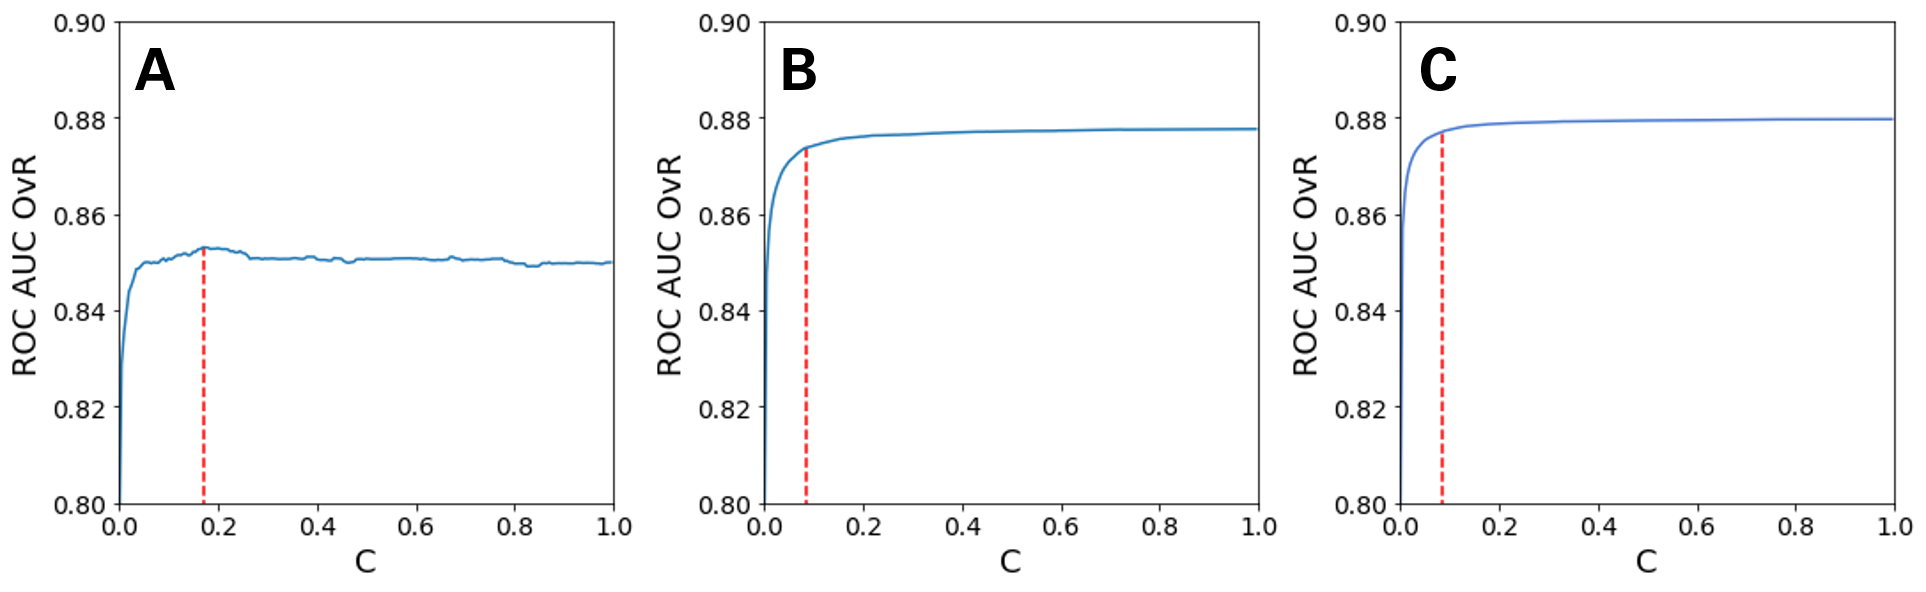
\includegraphics[width=\textwidth]{templates/images/Figure-LR_C_tuning.png}
\singlespacing
\caption[Logistic regression hyperparameter tuning]{Tuning plots for logistic regression C hyperparameter based on ROC AUC OvR values for A. WDS,  B. WDS4, and C. WDS8. WDS value selected from the plot maximum. Selections for WDS4 and WDS8 target the elbow of the curve.}
\label{fig:logreg_hp_tuning}
\end{figure}

The logistic regression (LR) model used in this analysis \citep{pedregosa_scikit-learn_2011} includes a single tunable hyperparameter, \verb|C|. Rather than rely on the pre-split training and validation subsets defined in Section \ref{ch3:strat_sample} to tune this hyperparameter, the subsets were re-combined and stratified-sampled as part of a 10-fold CV process. ROC AUC OvR was used as the scoring metric. Results vary for the different input data sets; CV results for WDS show a clear maximum AUC marking the optimal value for \verb|C|, whereas CV for WDS4 and WDS8 demonstrate a leveling-off trend and the optimal value must be selected near the elbow (Figure \ref{fig:logreg_hp_tuning}). The chosen \verb|C| values for WDS, WDS4, and WDS8 are listed in Table \ref{tab:logreg_tuning}.

Out-of-sample AUC values calculated on the testing subset indicate WDS4 has the best performance of the three data sets. Figure \ref{fig:logreg_coefs} shows a plot of the feature coefficients for each of the class-specific OvR classifiers in the WDS4 model. Longer bars indicate larger influence on the model prediction. The top 5 features across the four classifiers are Si Geothermometer Temperature, Basement Depth, Drainage Density, Spring Density, and Volcanic Dike Density.

\begin{figure}%[!htp]
\centering
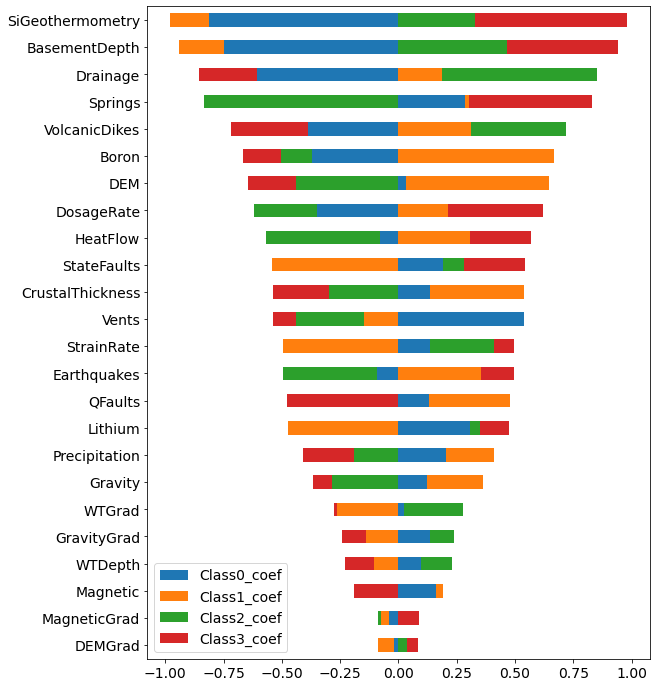
\includegraphics[width=\textwidth]{templates/images/Figure-LR-coefficients.png}
\singlespacing
\caption[Logistic regression feature coefficients]{Logistic regression coefficient values for OvR classifiers trained on WDS4. Stacked bar length is a proxy for overall importance to the classification.}
\label{fig:logreg_coefs}
\end{figure}

\subsection{Feature Selection} \label{ch5:lr_feature_selection}
Figure \ref{fig:logreg_rfe} presents the results of Recursive Feature Selection (RFE, see Section \ref{ch3:lr_rfe}) applied to the LR model for WDS4. Based on the plot, a local peak in AUC occurs when 18 features are used. Adding the remaining features results in small gains in AUC, but with diminishing returns for six additional features of complexity. Using this threshold, the data layers removed from the model include: DEM Gradient, Gravity Gradient, Magnetic Anomaly, Magnetic Anomaly Gradient, Water Table Depth, and Average Precipitation. Note that Average Precipitation appears higher on the coefficients plot (Figure \ref{fig:logreg_coefs}) than other features that were not removed. Since RFE iteratively removes predictors and refits the model, relative coefficients can change, particularly if there was collinearity with a removed variable.

\begin{figure}[!htp]
\centering
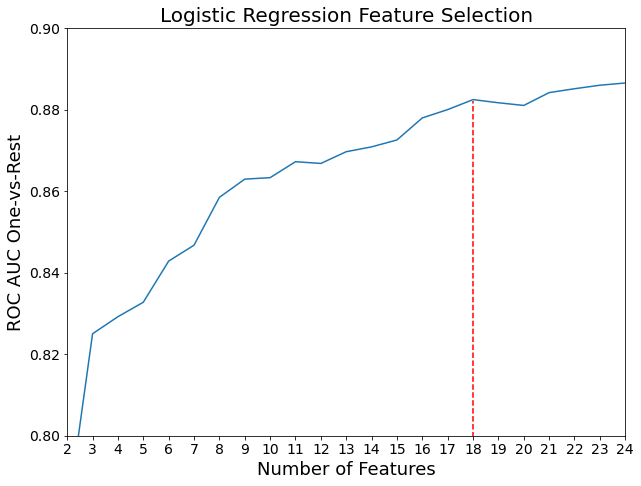
\includegraphics[width=0.70\textwidth]{templates/images/Figure-LR_feature_selection.png}
\singlespacing
\caption[Logistic regression feature selection]{Logistic regression feature selection using RFE and WDS4. Red dashed line indicates the chosen number of features to use for the LR model.}
\label{fig:logreg_rfe}
\end{figure}

\subsection{Optimized Model Results}\label{ch5:lr_results}
%\begin{wrapfigure}{R}{0.50\linewidth}
\begin{figure}%{R}{0.50\linewidth}
\centering
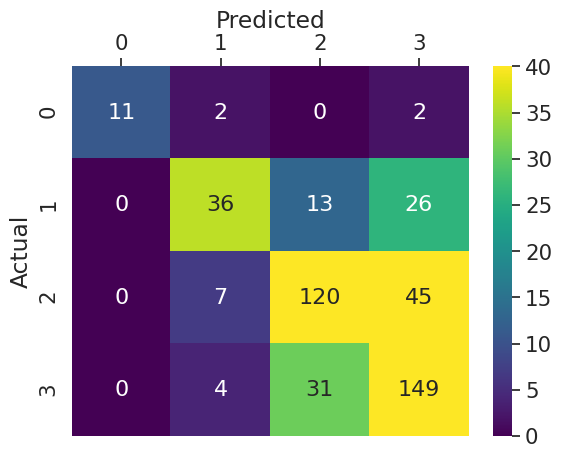
\includegraphics[width=0.5\textwidth]{templates/images/Figure-LR-ConfusionMatrix.png}
\singlespacing
\caption[Logistic regression confusion matrix]{Confusion matrix for the tuned LR model trained on WDS4.}
\label{fig:logreg_conf_matrix}
%\end{wrapfigure}
\end{figure}
A final LR model trained on WDS4 was constructed using the tuned C hyperparameter and reduced feature set from RFE. The confusion matrix suggests shows moderately good model performance (Figure \ref{fig:logreg_conf_matrix}). Correct predictions for each of the four classes of geothermal gradient (TP) outnumber the misclassifications for those classes (FP). The model appears to struggle most with differentiating between class 2 and class 3 locations, which separate mid-grade (40-60 K/km) from high-grade gradients (>60 K/km), although there are a large number of misclassifications (26) of low-grade gradient as high-grade as well.

Figure \ref{fig:logreg_auc} plots the macro average, micro average, and individual class ROC curves. Class 0 (non-thermal) predictive ability is quite high, pulling the micro-average AUC up to 0.88.  The macro AUC value of 0.85 is more aligned with the performance for other classes, which range from an AUC of 0.79-0.83. The trade-off between Class 2 and Class 3 is apparent in how the curve shapes mirror each other.

\begin{figure}[!htp]
\centering
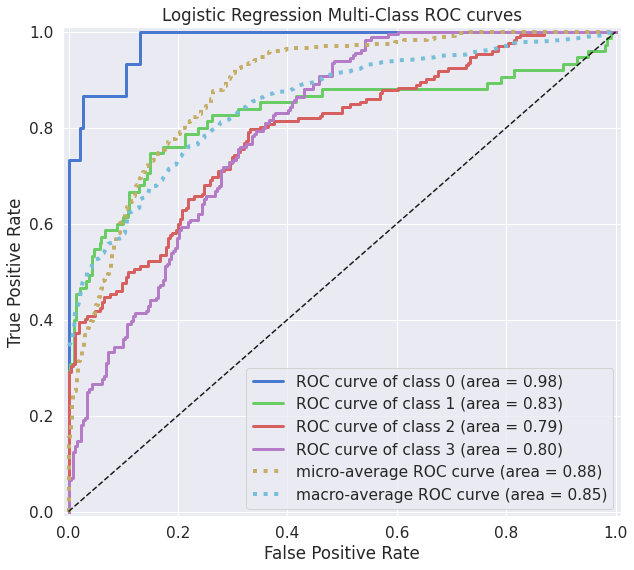
\includegraphics[width=0.6\textwidth]{templates/images/Figure-LR-AUC.png}
\singlespacing
\caption[Logistic regression ROC curves]{ROC curves for the tuned LR model trained on WDS4.}
\label{fig:logreg_auc}
\end{figure}

Model predictions for the study area are generated by passing the FDS through the final trained model. Class predictions are plotted in Figure \ref{fig:logreg_final_map}. High-grade geothermal gradient patches are concentrated to the southeast and through the center of the AOI. Smaller high-grade regions are observed along the southwest state boundary, following the Rio Grande River to the northeast, and a smaller patch directly to the north.  Comparing this result to the Southwestern NM PFA geothermal gradient data layer from \citet{bielicki_hydrogeolgic_2015}, high-grade predictions match in general spatial location except for the predicted patches to the north. The LR model tends to predict more widespread and spatially-continuous high-grade regions, while under-predicting lower gradient regions to the north, east, and mid-AOI near the Rio Grande River compared to the PFA layer.

\begin{figure}[!htp]
\centering
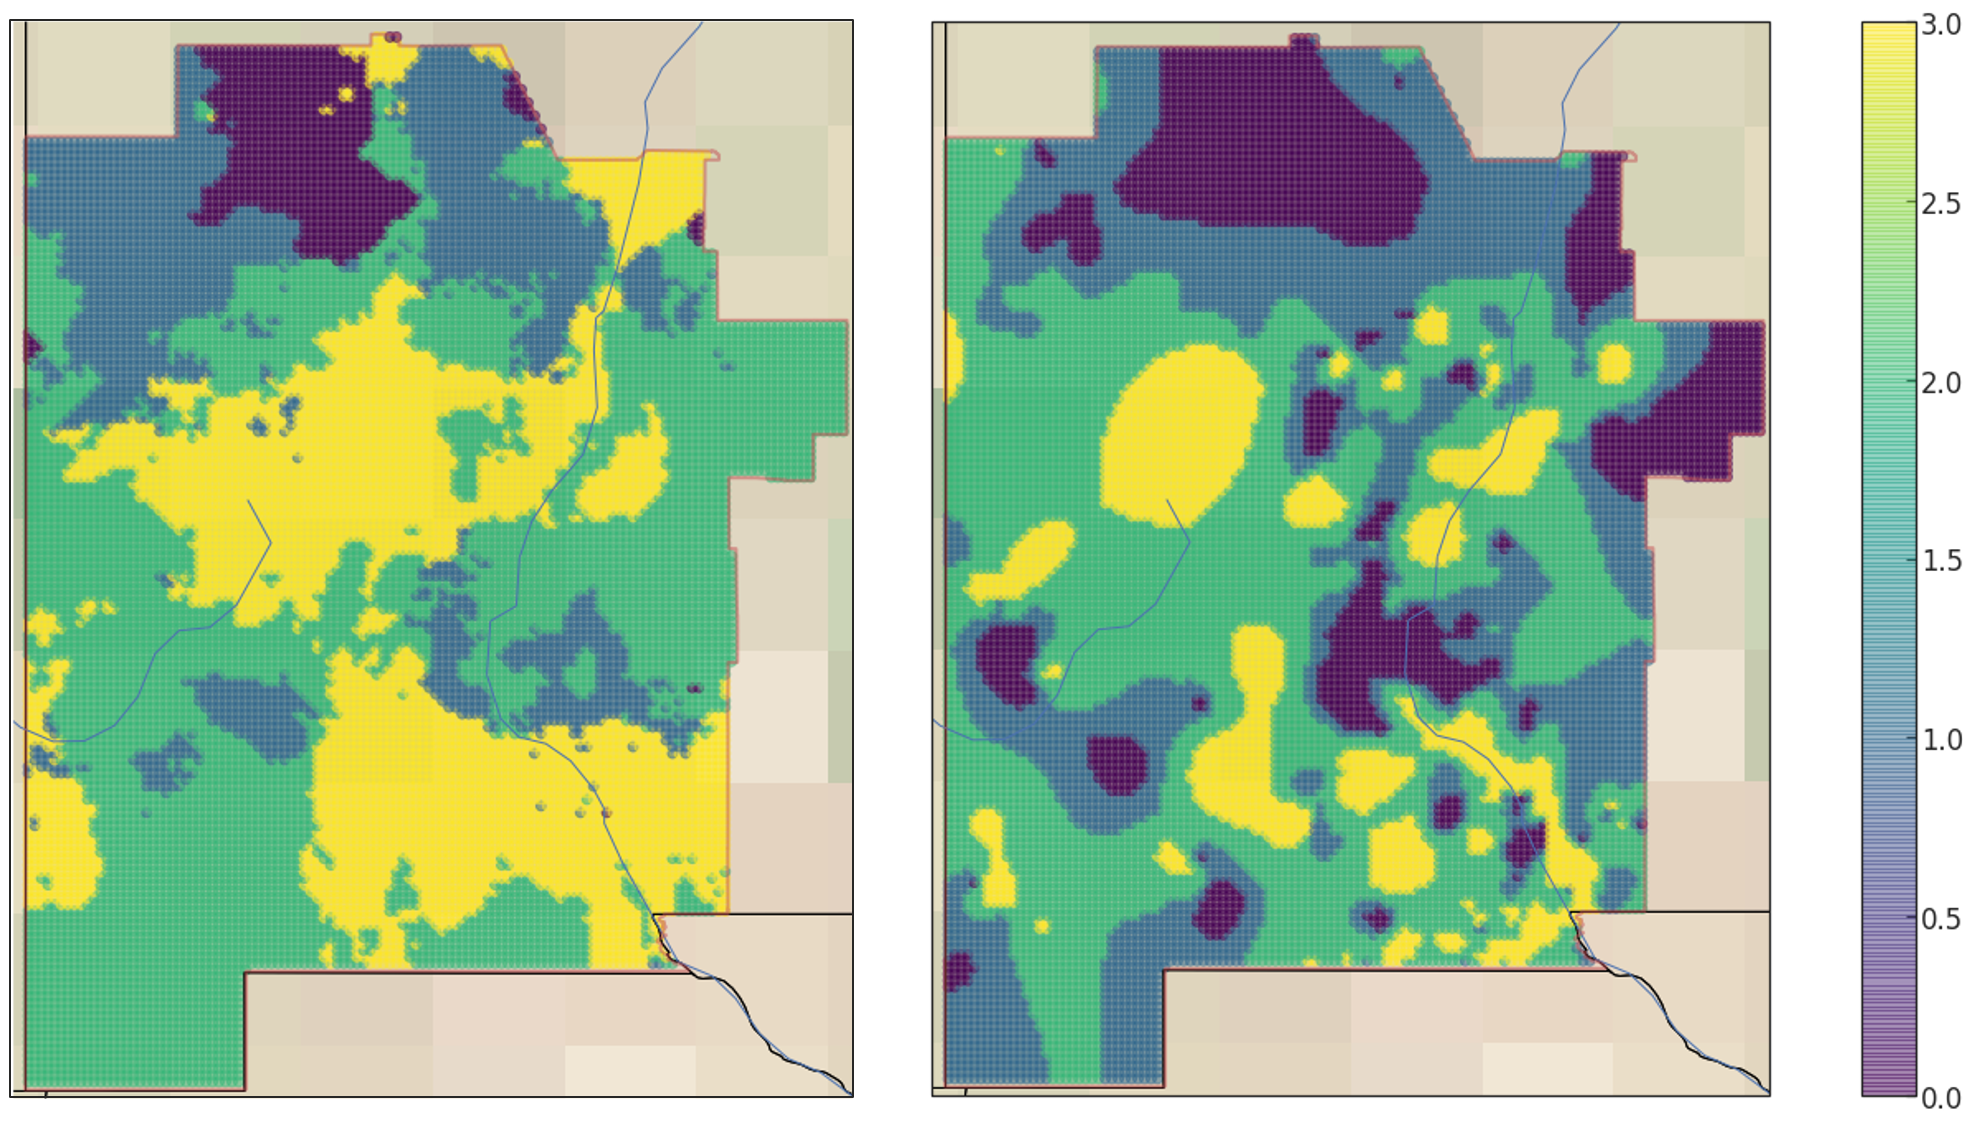
\includegraphics[width=\textwidth]{templates/images/Figure-LR-FinalMap_Joint.png}
\caption[Logistic regression prediction map]{Left: Map predictions of geothermal gradient class from the tuned LR model trained on WDS4. Right: geothermal gradient data layer from Southwestern NM PFA study \protect\citep{bielicki_hydrogeolgic_2015}.}
\label{fig:logreg_final_map}
\end{figure}

\section{Decision Trees}\label{ch5:dtree_model}
\subsection{Hyperparameter Tuning}\label{ch5:dtree_tuning}
Stepping up in complexity, the scikit-learn version of the decision tree (DT) classifier has over ten adjustable hyperparameters for tuning performance \citep{pedregosa_scikit-learn_2011}. Here, six hyperparameters are tuned using the stratified k-Fold CV method described in Section \ref{ch3:strat_kfold_cv}, with 10 folds and the multi-class OvR ROC AUC as the scoring metric. Figures illustrate the tuning results for WDS4.

First, \verb|max_depth| and \verb|criterion| were tuned together. \verb|max_depth| limits tree expansion by capping the number of parameter evaluations (tree nodes) considered before a classification label assignment. \verb|criterion| refers to the quality metric used for tree construction, i.e. Gini index or Entropy. The similarity of AUC curves in Figure \ref{fig:dtree_maxdepth} illustrates the relative insensitivity the classifier has to \verb|criterion|, while \verb|max_depth| plays a stronger role in performance. A maximum AUC score is observed with a \verb|max_depth| of 8 and \verb|criterion| choice of Entropy.

\begin{figure}[!htp]
\centering
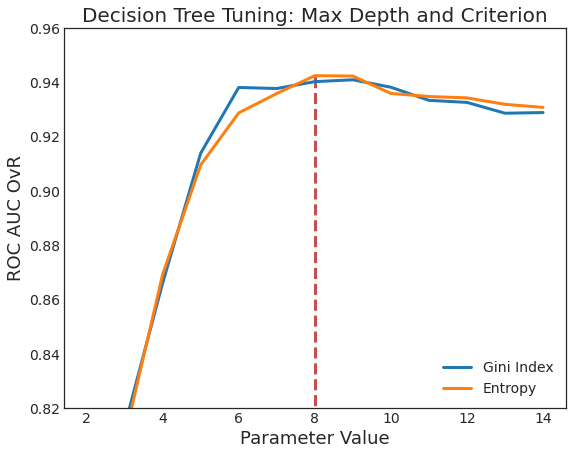
\includegraphics[width=.6\textwidth]{templates/images/Figure-DT_tuning_maxdepth_criterion.png}
\caption[Decision tree max depth tuning]{Results from stratified k-fold cross validation tuning of the max\_depth and criterion hyperparameters using WDS4. The red dashed line indicates the selected max\_depth value.}
\label{fig:dtree_maxdepth}
\end{figure}

Next, \verb|min_samples_leaf| and \verb|min_samples_split| were tuned in succession. The former defines the minimum number of samples from the training set that must be assigned to a leaf node for that leaf to remain in the tree. The latter sets a minimum number of training set samples that must be assigned to a node before that node can be considered for a split. Figure \ref{fig:dtree_min_samples} illustrates the selected parameter values, defined by maxima in the AUC vs. parameter value plots. The insensitivity of the classifier to low values of \verb|min_samples_split| demonstrates the cascading influence of the hyperparameters in this tuning flow. When \verb|min_samples_leaf| is set to 8, a split can only occur when the node being split has at least 16 observations, so any \verb|min_samples_split| value under 16 does not influence tree construction. 

\begin{figure}[!htp]
\centering
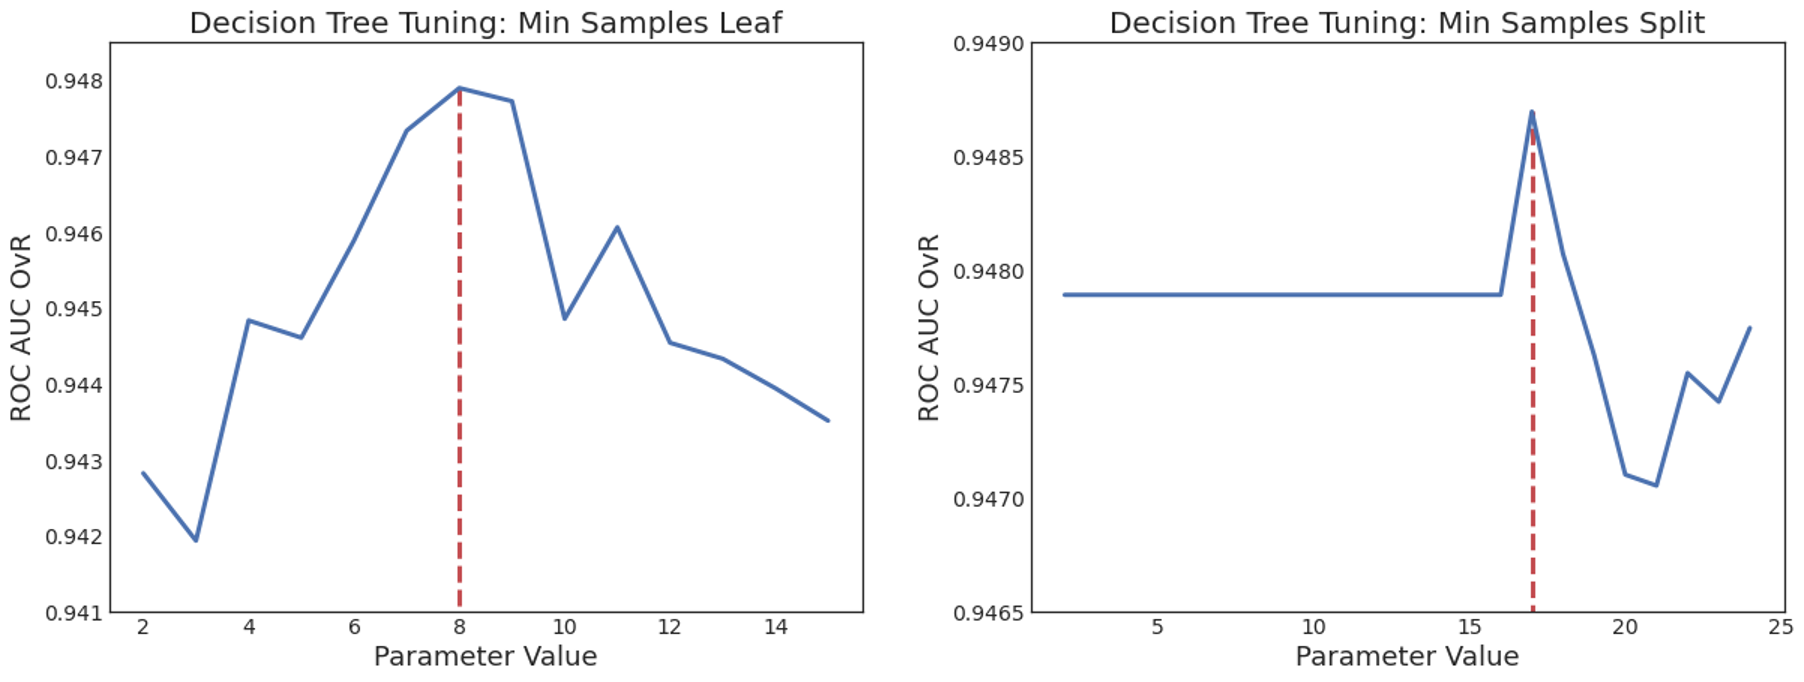
\includegraphics[width=\textwidth]{templates/images/Figure-DT_tuning_min_samp_leaf_split.png}
\caption[Decision tree min samples tuning]{Results from stratified k-fold cross validation tuning of the min\_samples\_leaf (Left) and min\_samples\_split (Right) hyperparameters using WDS4. The red dashed lines indicate the selected values.}
\label{fig:dtree_min_samples}
\end{figure}

One optimization trick when training DT models is to only consider a subset of the features when splitting decision tree nodes. This also adds an element of randomness to tree construction, so decision trees can differ when constructed on the same training data depending on how many features were considered for each split. No clear maximum appears in the AUC plot for \verb|max_features| (Figure \ref{fig:dtree_max_features}), so a value of 8 was selected using the elbow criterion. \verb|max_features| can also cause problems when performing feature selection if the feature count drops below the \verb|max_features| value, so care must be taken in using this parameter.

\begin{figure}[!htp]
\centering
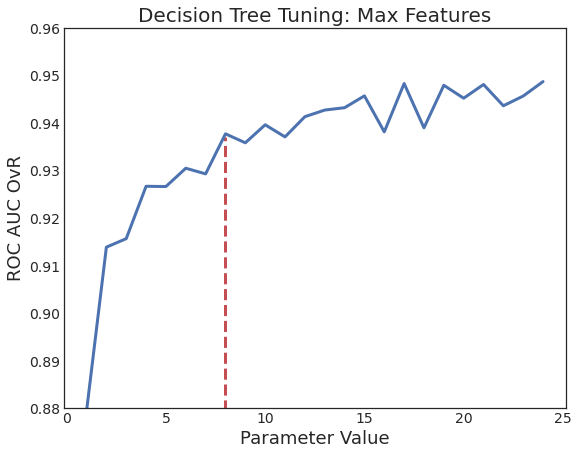
\includegraphics[width=.6\textwidth]{templates/images/Figure-DT_tuning_max_features.png}
\caption[Decision tree max features tuning]{Results from stratified k-fold cross validation tuning of the max\_features hyperparameter using WDS4. The red dashed line indicates the selected value, conservatively selected at the high end of the ``elbow'' in the plot.}
\label{fig:dtree_max_features}
\end{figure}

The final hyperparameter, \verb|ccp_alpha|, controls the trade-off between model fit and complexity during the tree-pruning backward pass of tree construction. As the alpha value increases from zero, the difference between in-sample (training) and out-of-sample (validation) performance decreases, but so does the overall performance of the classifier on the validation subset. Figure \ref{fig:dtree_alpha} shows a clear minima in train-validate AUC difference, however the validation set performance drops from 0.95 to under 0.85 when using this value for \verb|ccp_alpha|. The default value of \verb|ccp_alpha| = 0.0 is chosen instead to maximize out-of-sample AUC.

\begin{figure}[!htp]
\centering
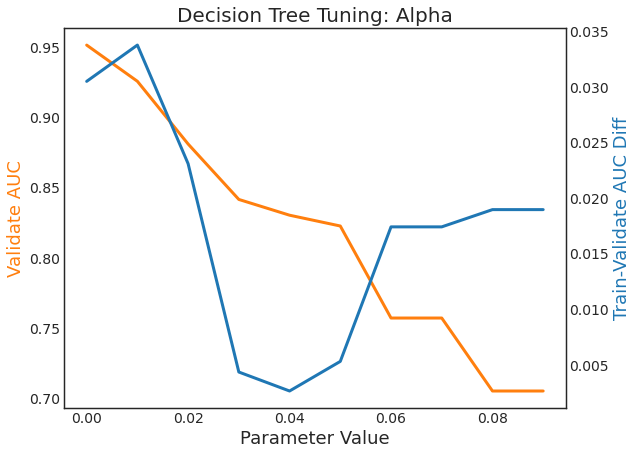
\includegraphics[width=.6\textwidth]{templates/images/Figure-DT_tuning_alpha.png}
\caption[Decision tree alpha tuning]{Results from stratified k-fold cross validation tuning of the ccp\_alpha hyperparameter. The orange line plots the validation subset AUC. The blue line plots the difference in AUC between training and validation subsets.}
\label{fig:dtree_alpha}
\end{figure}

Final hyperparameter values and performance results for WDS, WDS4, and WDS8 are listed in Table \ref{tab:dtree_tuning}. The data augmentation strategy behind WDS4 and WDS8 results in a significant improvement in classifier performance over the original WDS.

\begin{table}[!htp]
\centering
\begin{tabular}{l|c|c|c|}
\cline{2-4}
                                          & \textbf{WDS} & \textbf{WDS4} & \textbf{WDS8} \\ \hline
\multicolumn{1}{|l|}{\textbf{criterion}}           & Gini & Entropy & Entropy \\ \hline
\multicolumn{1}{|l|}{\textbf{max\_depth}}          & 5    & 8    & 10   \\ \hline
\multicolumn{1}{|l|}{\textbf{min\_samples\_leaf}}  & 7    & 8    & 10   \\ \hline
\multicolumn{1}{|l|}{\textbf{min\_samples\_split}} & 21   & 17   & 24   \\ \hline
\multicolumn{1}{|l|}{\textbf{max\_features}}       & 5    & 8    & 6    \\ \hline
\multicolumn{1}{|l|}{\textbf{ccp\_alpha}}          & 0    & 0    & 0    \\ \hline
\multicolumn{1}{|l|}{\textbf{Accuracy$_{train}$}}  & 0.767 & 0.881 & 0.880 \\ \hline
\multicolumn{1}{|l|}{\textbf{Accuracy$_{test}$}}   & 0.600 & 0.818 & 0.838 \\ \hline
\multicolumn{1}{|l|}{\textbf{AUC$_{train}$}}       & 0.909 & 0.982 & 0.985 \\ \hline
\multicolumn{1}{|l|}{\textbf{AUC$_{test}$}}        & 0.814 & 0.944 & 0.961 \\ \hline
\end{tabular}
\caption[Decision tree hyperparameter values]{Tuned hyperparameter selections and resulting decision tree model Accuracy and AUC for training and testing subsets of WDS, WDS4, and WDS8.}
\label{tab:dtree_tuning}
\end{table}

\subsection{Feature Selection}\label{ch5:dtree_feat_selection}
Figure \ref{fig:dtree_feat_import} shows the feature importances determined by models constructed using WDS, WDS4, and WDS8. Features are sorted on the sum of importance values across all 3 data sets. Although differences exist, Si Geothermometer Temperature tops the list as the most important predictor in all cases. And the bottom six features are also remarkably consistent across data sets: Water Table Depth, Water Table Gradient, Gravity Anomaly Gradient, Magnetic Anomaly, Magnetic Anomaly Gradient, and DEM Gradient. Dropping these features reduces the count to 18 features in total.

\begin{figure}[!htp]
\centering
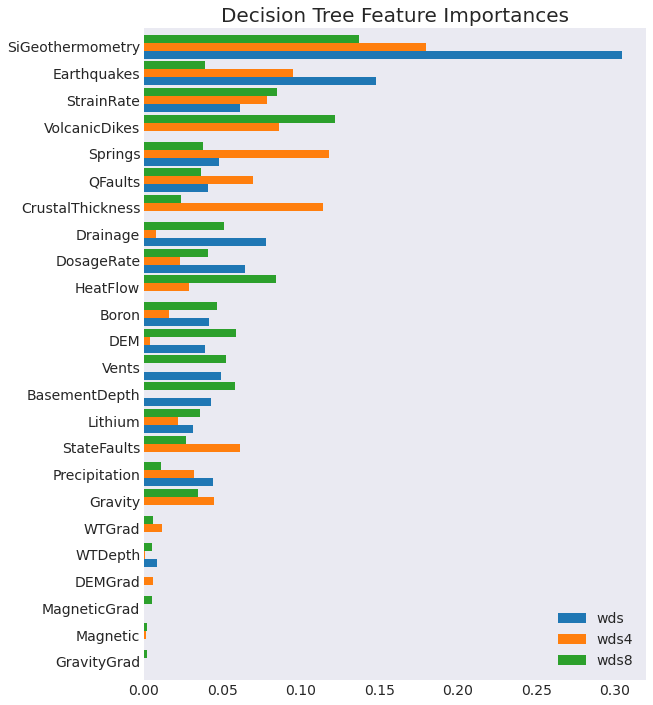
\includegraphics[width=\textwidth]{templates/images/Figure-DT_feature_importances_all.png}
\caption[Decision tree feature importances]{Decision tree feature importances for WDS, WDS4, and WDS8, sorted on the sum total importance across the 3 data sets.}
\label{fig:dtree_feat_import}
\end{figure}

\subsection{Optimized Model Results}
\begin{figure}[!htp]
\centering
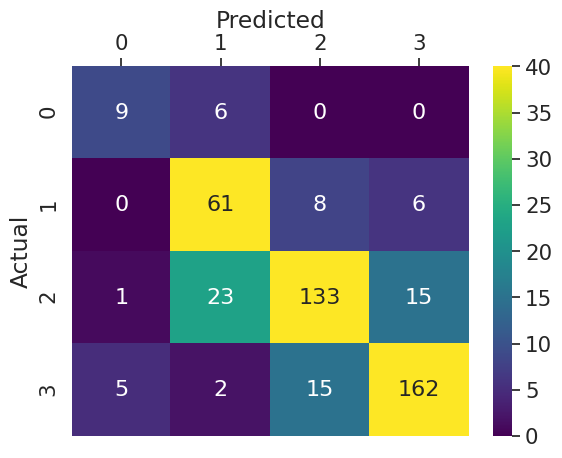
\includegraphics[width=0.5\textwidth]{templates/images/Figure-DT-ConfusionMatrix.png}
\singlespacing
\caption[Decision tree confusion matrix]{Confusion matrix for tuned DT model trained on WDS4.}
\label{fig:dtree_conf_matrix}
\end{figure}

A final DT model trained on WDS4 was constructed using the tuned hyperparameters and 18-predictor reduced feature set. The confusion matrix (Figure \ref{fig:dtree_conf_matrix}) demonstrates an improvement in model results over the logistic regression method. Low-grade gradient locations are correctly predicted for almost double the number of sites, and half as many misclassifications are observed between class 2 (mid-grade) and class 3 (high-grade) geothermal gradient as with the LR model.

Figure \ref{fig:dtree_auc} shows the macro average, micro average, and individual class DT ROC curves. All individual class AUC values exceed 0.90. Class 0 (non-thermal) continues to demonstrate the highest predictive performance (AUC=0.97), but class 3 (high-grade) predictive ability boosts micro-average AUC at higher decision thresholds, i.e., where the class 0 ROC curve steeply drops in TPR for FPR < 0.1. Class 2 (medium-grade) classification performance lags behind all other classes for the DT classifier.

\begin{figure}[!htp]
\centering
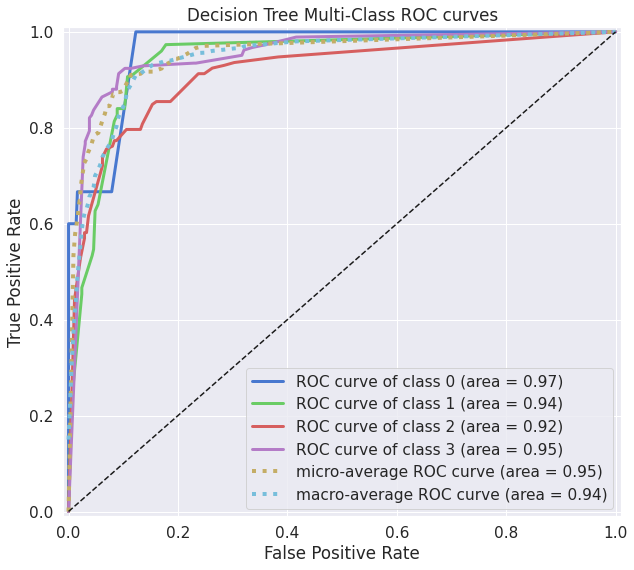
\includegraphics[width=0.6\textwidth]{templates/images/Figure-DT_AUC.png}
\caption[Decision tree ROC curves]{ROC curves for the tuned DT model trained on WDS4.}
\label{fig:dtree_auc}
\end{figure}

Model predictions for the study area are generated by passing the FDS through the DT model. Class assignments based on the OvR methodology are plotted in Figure \ref{fig:dtree_final_map}. The high-grade geothermal gradient patches to the southeast and central regions of the AOI are not as broad and continuous as in the LR model (Figure \ref{fig:logreg_final_map}). Predictions for low-grade gradient or non-thermal areas are concentrated to the NW in the Colorado Plateau and central-east where Rio Grade Rift province transitions into the Great Plains. The overall distribution of geothermal gradient classes is similar to the \citet{bielicki_hydrogeolgic_2015} PFA layer (Figure \ref{fig:dtree_final_map}) but with a greater apportionment of high-grade gradient areas and fewer low-grade or non-thermal locations in the DT model.

\begin{figure}[!htp]
\centering
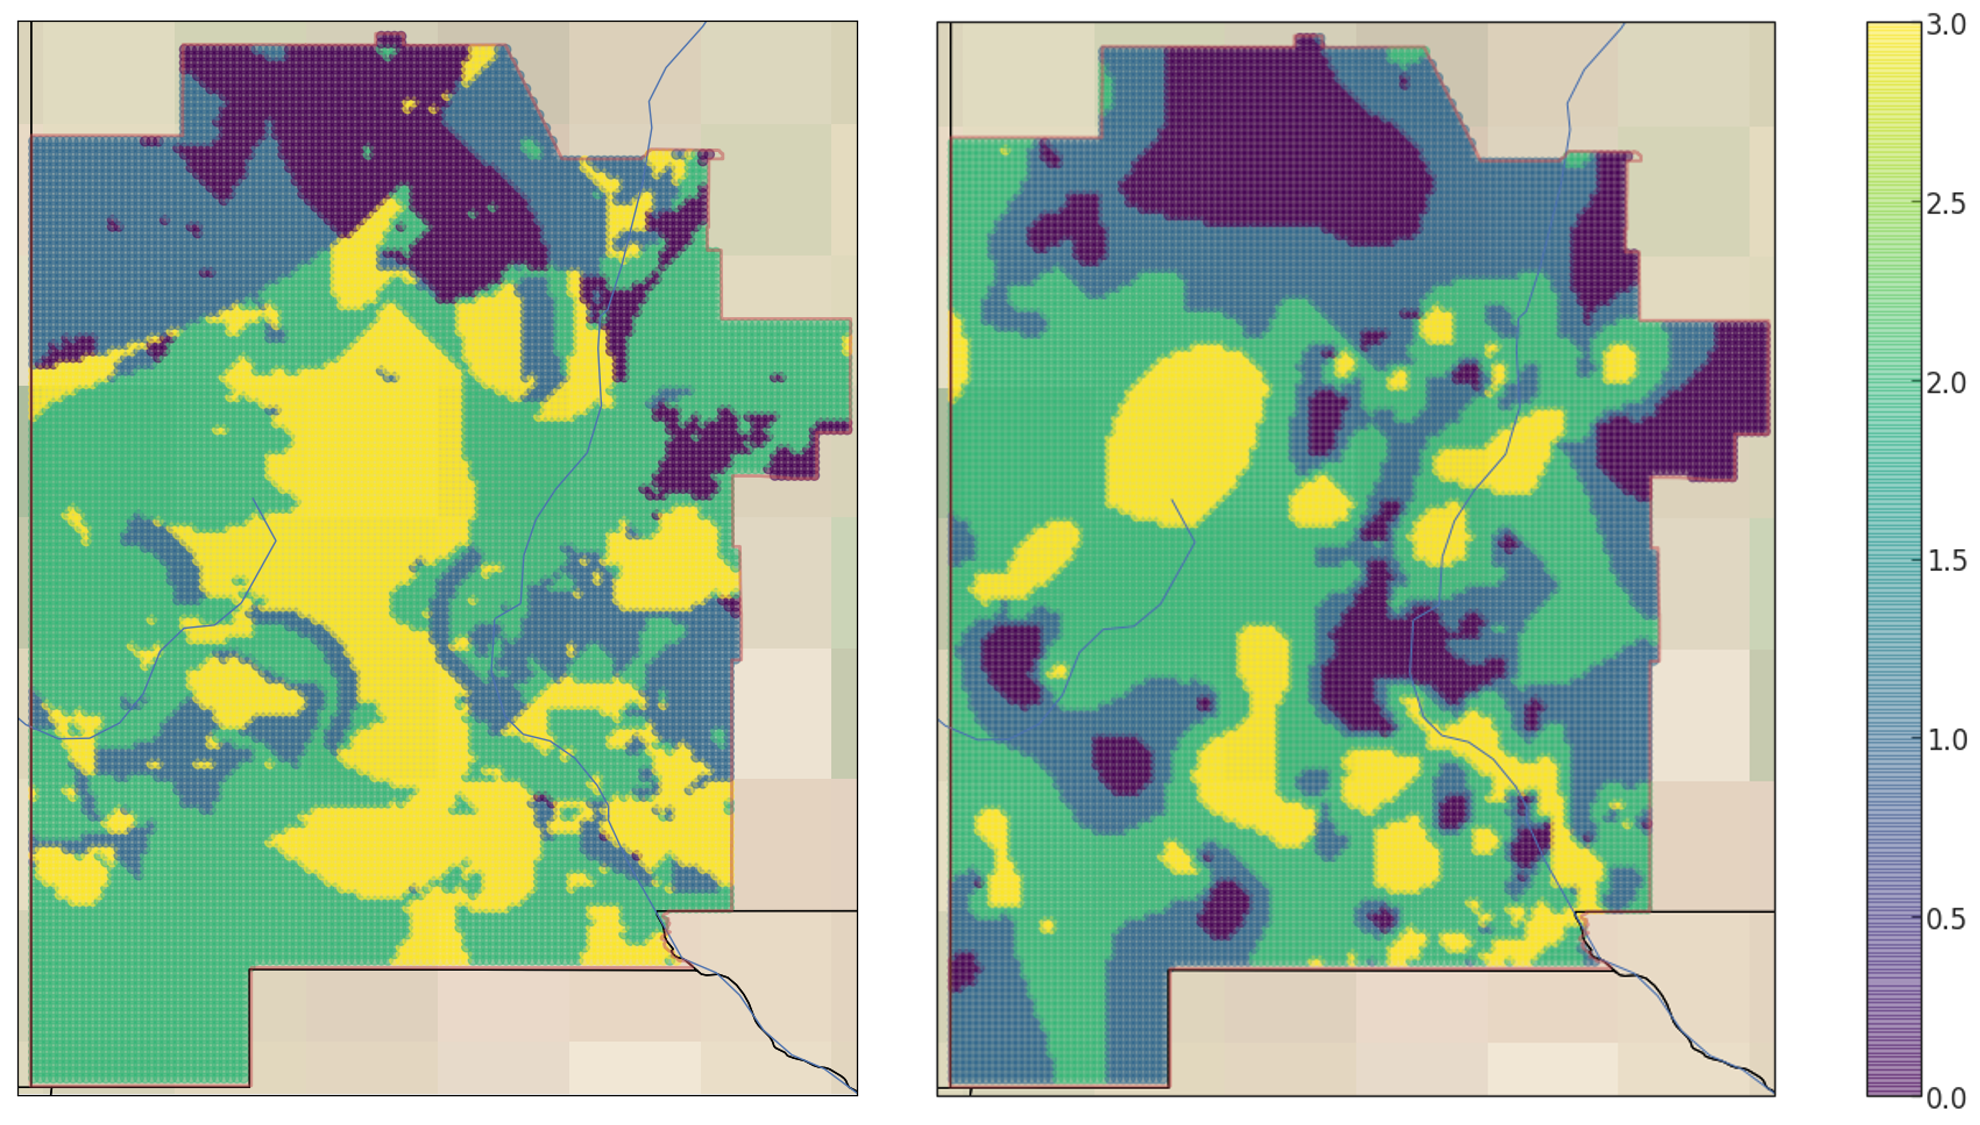
\includegraphics[width=\textwidth]{templates/images/Figure-DT-FinalMap_Joint.png}
\caption[Decision tree prediction map]{Left: Map predictions of geothermal gradient class from the tuned DT model trained on WDS4. Right: geothermal gradient data layer from Southwestern NM PFA study \protect\citep{bielicki_hydrogeolgic_2015}}
\label{fig:dtree_final_map}
\end{figure}

Note that if the random seed (fixed in this study for solution repeatability) is free to change and new DT models are constructed, some of the characteristics of this DT prediction will also change. In fact, one downside of the DT model is this randomness; decision trees will structurally rearrange each time the algorithm is run, even on the same training data, due to randomness in the node splitting process. Nevertheless, tree performance remains relatively stable overall. And the ability to plot and visually step through the model makes it one of the most accessible and interpretable methods to use (See Figure \ref{fig:dtree_viz}).

\begin{figure}[!htp]
\centering
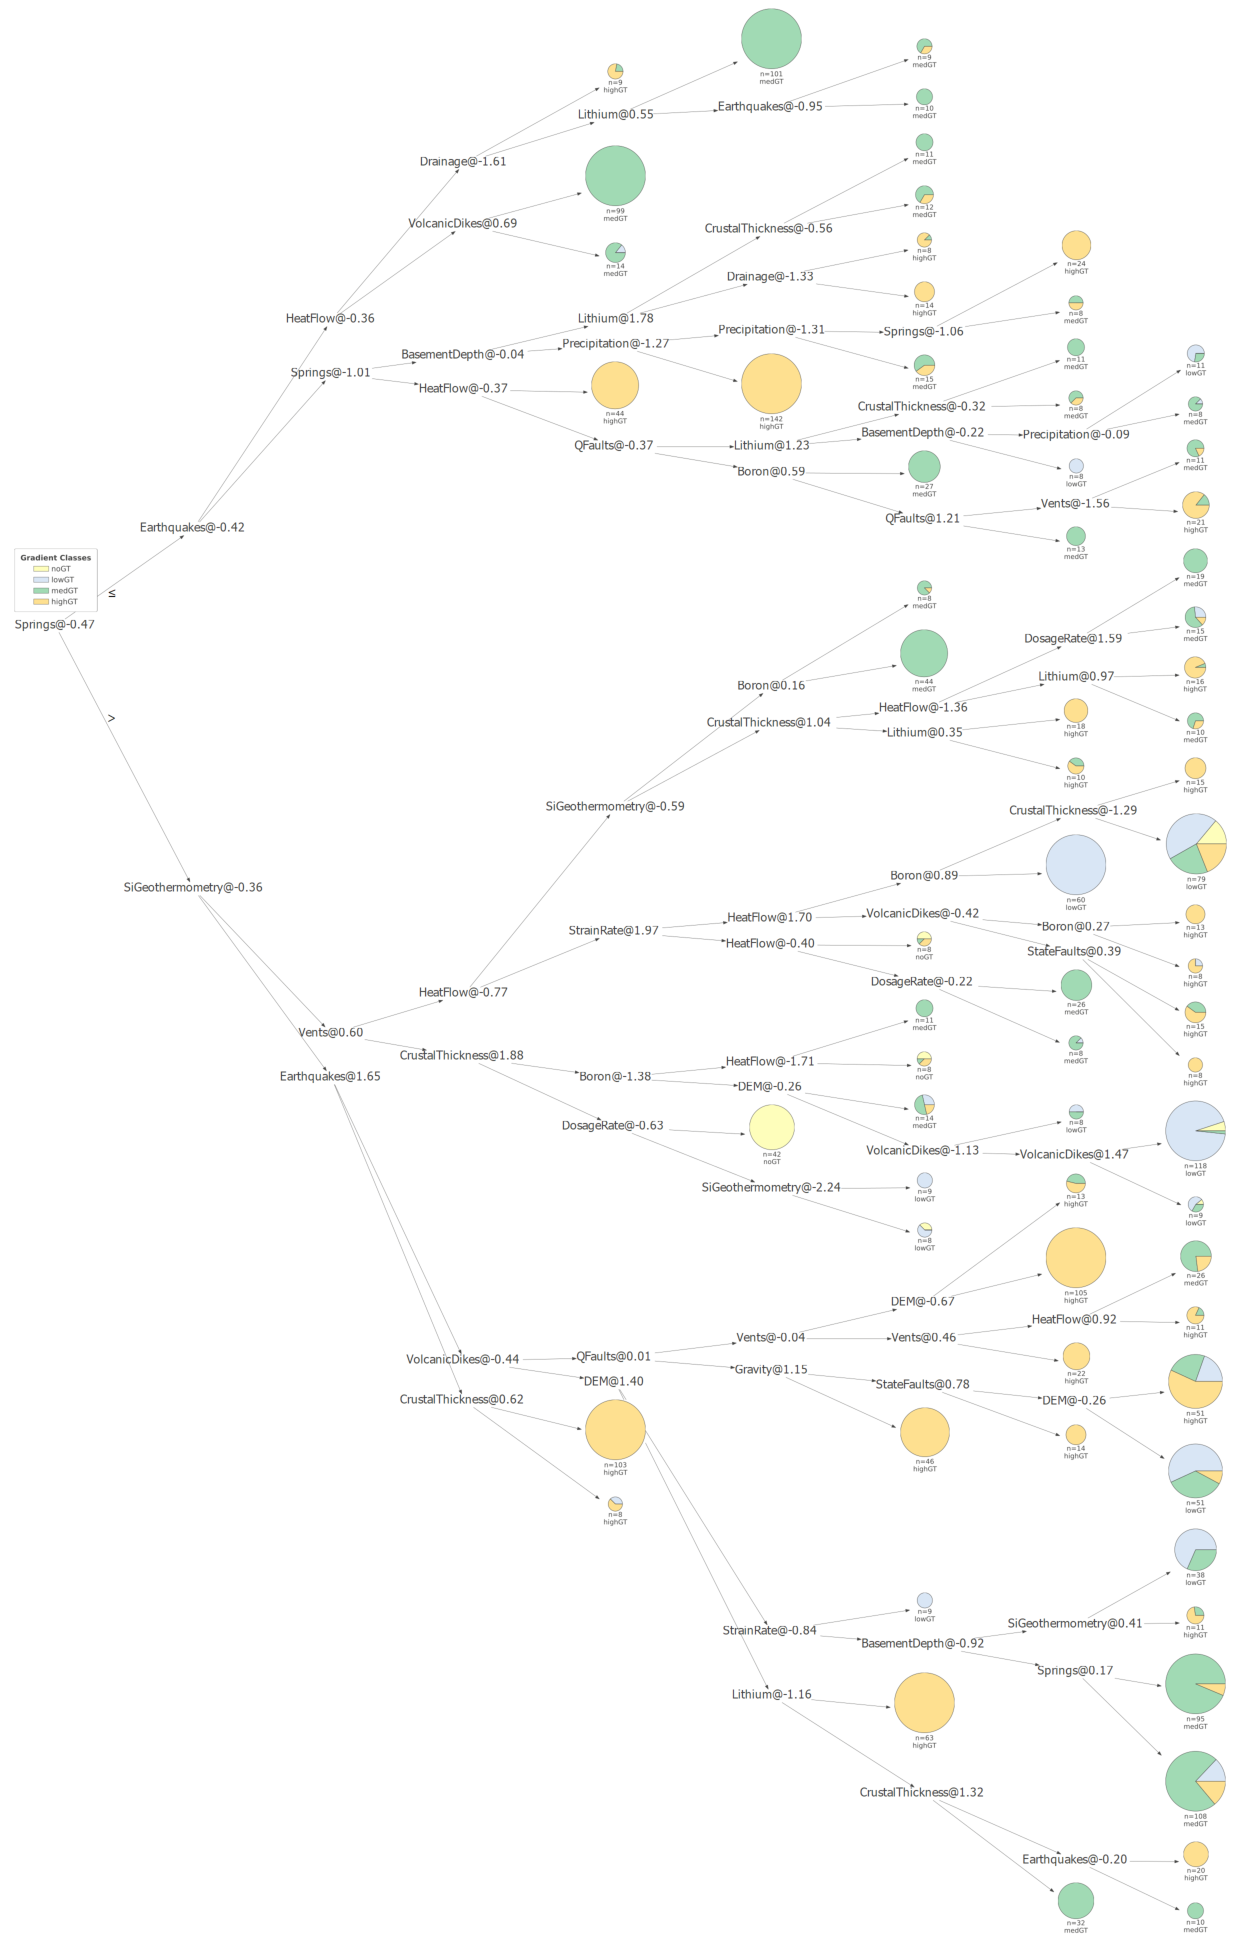
\includegraphics[height=0.85\textheight,keepaspectratio]{templates/images/Figure-DT_viz_portrait.pdf}
\caption[Decision tree visualization]{Decision tree visualization for the final decision tree model. Nodes are noted by predictor labels with their decision threshold. Bubbles illustrate the final distribution of classes in a leaf node, sized by number of observations. The majority class determines the classification label.}
\label{fig:dtree_viz}
\end{figure}

\section{Tree Ensembles (XGBoost)}\label{ch5:xgb_model}
\subsection{Hyperparameter Tuning}\label{ch5:xgb_tuning}
XGBoost comes with many of the same hyperparameters as decision trees, plus additional parameters related to boosting and optimization. With so many hyperparameters, tuning the model becomes a time-consuming and complex process. The method followed here was adapted from an online tutorial covering the topic \citep{jain_xgboost_2016}.
\\
\\
The following hyperparameters were tuned for the final model:
\begin{itemize}[itemsep=2pt]
    \item \textbf{Maximum depth}: similar to \verb|max_depth| for decision trees, restricts how deep each tree can grow during construction.
    \item \textbf{Minimum child weight}: sets a minimum weight requirement for a leaf nodes during the backward pass pruning process. Similar to \verb|min_samples_leaf| in decision trees, except this uses the XGB-specific weights noted in equation \ref{eq:xgb_objective}.
    \item \textbf{Gamma}: defines a minimum reduction in the loss function necessary for a split to be preserved during tree pruning. 
    \item \textbf{Learning rate}: also known as the shrinkage factor, scales the impact of each tree on the boosted model prediction, i.e., the $\alpha$ in equation \ref{eq:xgb_form}.
    \item \textbf{Lambda}: L2 regularization term on the leaf scores, i.e., the $\lambda$ in equations \ref{eq:xgb_objective} and \ref{eq:xgb_obj_simple}.
    \item \textbf{Subsample}: defines the fraction of observations in the full training set that are randomly selected as a limited training set for each tree.
    \item \textbf{Column sample by tree}: sets the fraction of predictors in the full training set that are randomly selected as a limited feature set for constructing each tree.
    \item \textbf{Number of estimators}: controls the number of sequential trees in the model, i.e., B in equation \ref{eq:xgb_form}.
    \item \textbf{Scale positive weight}: scales the gradient for the positive class to influence model corrections during training, useful for imbalanced classification.
\end{itemize}

The preferred method of tuning for XGBoost is the cross-validation strategy described in Section \ref{ch3:strat_kfold_cv}. Since this method uses the input data to both train and validate, the pre-generated training and validation subsets (Table \ref{tab:stratified_split_counts}) were re-combined before using CV. An initial trial-and-error testing of different parameter combinations found the best starting values for \verb|learning_rate| and \verb|n_estimators| were 0.01 and 200, respectively. Higher learning rates like those suggested by \citet{jain_xgboost_2016} led to a nearly perfect-fitting model before hyperparameters could be tuned, and more estimators created undesirably long training times. In the figures and discussion that follow, results are described for WDS4. Full results for all three data sets are provided in Table \ref{tab:xgb_tuning}.

\begin{figure}[!htp]
\centering
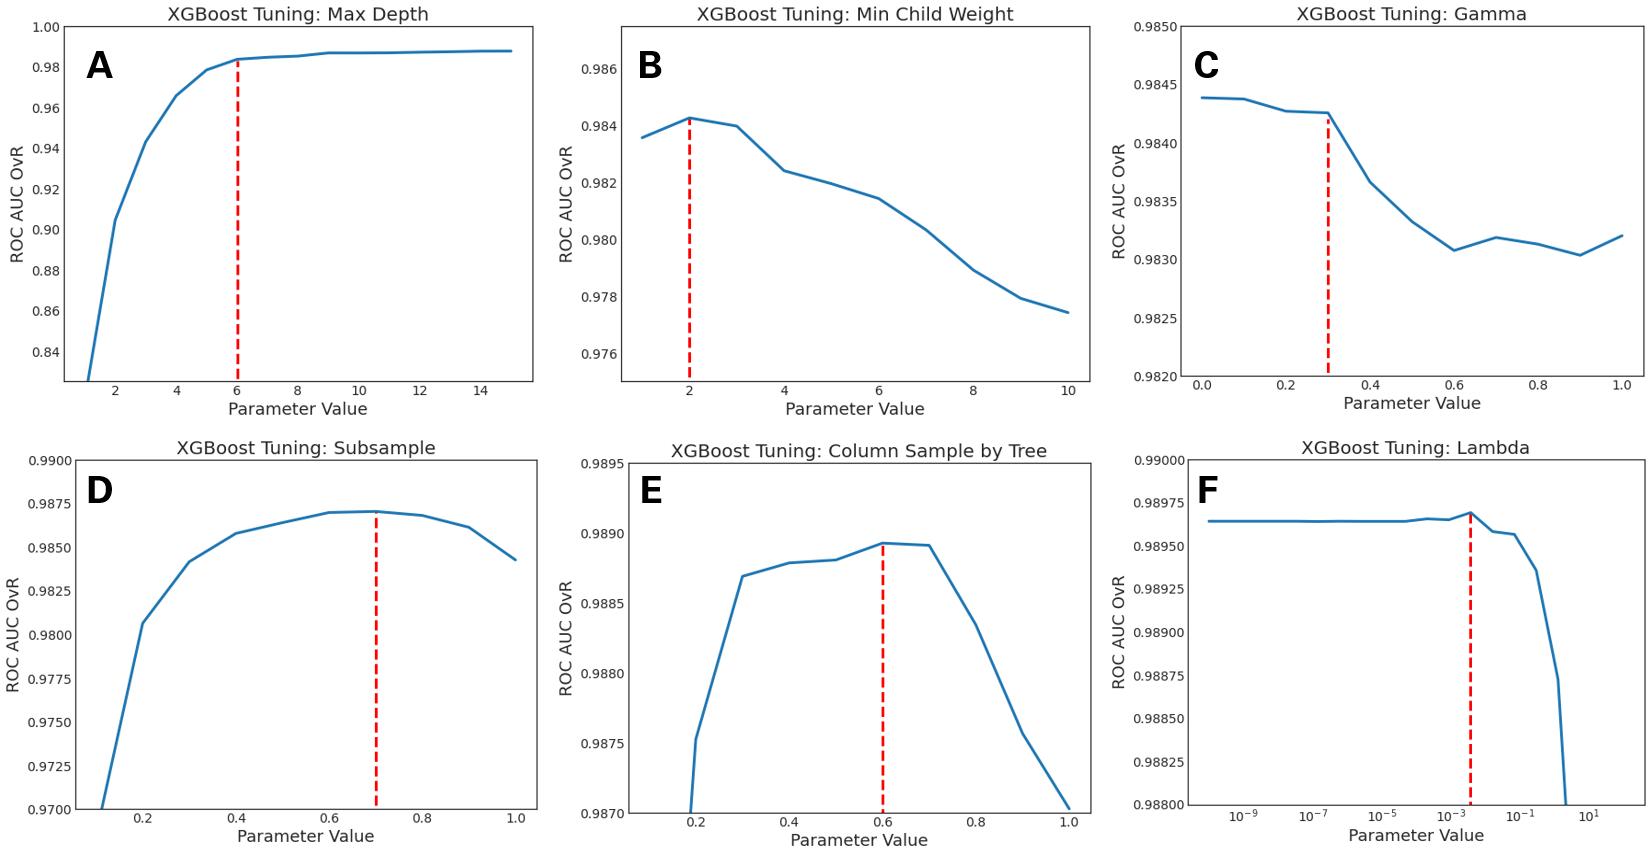
\includegraphics[width=\textwidth]{templates/images/Figure-XGB_Hyperparameters.png}
\caption[XGBoost hyperparameter tuning]{Hyperparameter tuning results for XGBoost modeling. A. max\_depth, B. min\_child\_weight, C. gamma, D. subsample, E. colsample\_bytree, F. lambda. Red dashed lines indicate values selected for the final model.}
\label{fig:xgb_hyperparam}
\end{figure}

XGBoost hyperparameters were tuned in succession using 10-fold stratified CV and a grid search across potential parameter values. Figure \ref{fig:xgb_hyperparam}A shows the results for \verb|max_depth|. As noted when tuning the DT model (Section \ref{ch5:dtree_tuning}), \verb|max_depth| does not exhibit a clear maximum in the AUC vs. hyperparameter value plot. A preferred value of 6 was instead selected using the elbow criterion.

Next, tuning was performed on the \verb|min_child_weight| hyperparameter. Results of the 10-fold stratified CV method revealed a clear maximum AUC when \verb|min_child_weight| is 2 (Figure \ref{fig:xgb_hyperparam}B).

XGBoost uses a default value of 0 for the \verb|gamma| hyperparameter, which controls when tree partitioning should stop based on loss reduction. Cross-validation shows nearly level AUC values out to \verb|gamma| = $3.8 \text{x} 10^-3$, after which the AUC score quickly drops. This threshold value was selected for the model (Figure \ref{fig:xgb_hyperparam}C).

Trees in the XGBoost model can be trained on random subsets of training data observations and individual feature columns. Tuning of \verb|subsample| identified a broad maximum in AUC when using 60-80\% of the training observations to build decision trees (Figure \ref{fig:xgb_hyperparam}D). The selected \verb|subsample| value is 70\%. For \verb|colsample_bytree|, the best AUC results occur when 60\% of the features are included in the training (Figure \ref{fig:xgb_hyperparam}E). A value below 100\% for \verb|colsample_bytree| suggests removing features based on estimates of feature importance could be beneficial, as previously discussed for both logistic regression (Section \ref{ch5:lr_feature_selection}) and decision trees (Section \ref{ch5:dtree_feat_selection}). A more robust method for feature attribution and selection using Shapley values is considered in Section \ref{ch5:xgb_feature_selection}.

Tuning results show model AUC remains flat, then quickly drops for increasing values of the \verb|lambda| hyperparameter (Figure \ref{fig:xgb_hyperparam}E). This behavior shows how higher levels of regularization can cause data underfitting. The largest \verb|lambda| value just short of this drop-off was selected for the final model.

\verb|scale_pos_weight| was similarly tuned, but AUC results remained unchanged for all hyperparameter values tested. The multi-class XGBoost classifier appears to be insensitive to this hyperparameter.

As a final step in model tuning, \verb|learning_rate| was decreased to 0.005 and \verb|n_estimators| increased to 1000.  Using the slower learning rate reduces the chance of overfitting the training data, while the increased number of sequential trees in the model ensures a good fit can be learned. 
Final hyperparameter values and performance results for WDS, WDS4, and WDS8 are listed in Table \ref{tab:xgb_tuning}. Once again, WDS4 and WDS8 out-perform the original WDS based on AUC values for the test set.

\begin{table}[!htp]
    \centering
    \begin{tabular}{l|c|c|c|}
    \cline{2-4}
                                             & \textbf{WDS}   & \textbf{WDS4}    & \textbf{WDS8}  \\ \hline
    \multicolumn{1}{|l|}{\textbf{max\_depth}}         & 6     & 6       & 6     \\ \hline
    \multicolumn{1}{|l|}{\textbf{min\_child\_weigh}t} & 2     & 2       & 5     \\ \hline
    \multicolumn{1}{|l|}{\textbf{gamma}}              & 0.5   & 0.3     & 0.5   \\ \hline
    \multicolumn{1}{|l|}{\textbf{subsample}}          & 0.8   & 0.7     & 0.7   \\ \hline
    \multicolumn{1}{|l|}{\textbf{colsample\_bytree}}  & 0.4   & 0.6     & 0.6   \\ \hline
    \multicolumn{1}{|l|}{\textbf{reg\_lambda}}        & 0.30  & 3.8E-03 & 1.3   \\ \hline
    \multicolumn{1}{|l|}{\textbf{scale\_pos\_weight}} & 0.0   & 0.0     & 0.0   \\ \hline
    \multicolumn{1}{|l|}{\textbf{learning\_rate}}     & 0.005 & 0.005   & 0.005 \\ \hline
    \multicolumn{1}{|l|}{\textbf{n\_estimators}}      & 1000  & 1000    & 1500  \\ \hline
    \multicolumn{1}{|l|}{\textbf{Accuracy$_{train}$}} & 0.995 & 0.991   & 0.988 \\ \hline
    \multicolumn{1}{|l|}{\textbf{Accuracy$_{test}$}}  & 0.767 & 0.944   & 0.955 \\ \hline
    \multicolumn{1}{|l|}{\textbf{AUC$_{train}$}}      & 1.000 & 1.000   & 1.000 \\ \hline
    \multicolumn{1}{|l|}{\textbf{AUC$_{test}$}}       & 0.938 & 0.995   & 0.995 \\ \hline
    \end{tabular}
    \caption[XGBoost hyperparameter values]{Tuned hyperparameter selections and resulting XGBoost model AUC for training and test subsets of WDS, WDS4, and WDS8.}
    \label{tab:xgb_tuning}
\end{table}

\subsection{Feature Selection}\label{ch5:xgb_feature_selection}

\begin{figure}[htp]
\centering
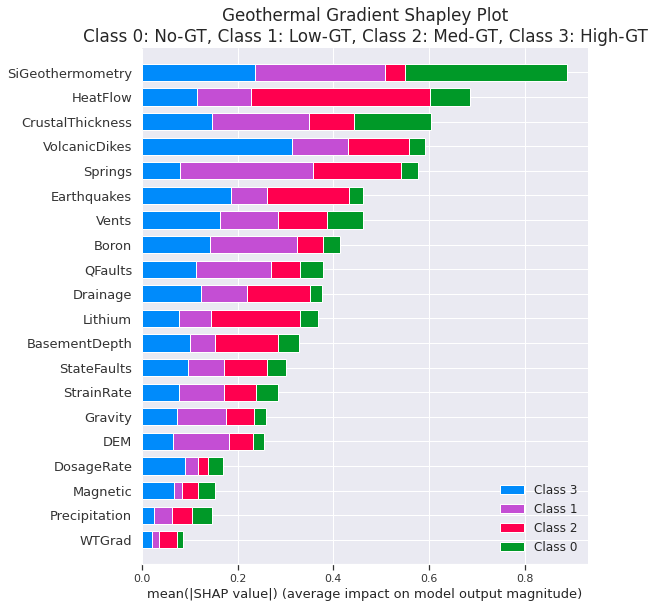
\includegraphics[width=\textwidth]{templates/images/Figure-Shapley.png}
\caption[XGBoost SHAP values]{SHAP values for the XGBoost classifier derived using the test subset of WBS4. Step-like tiers in cumulative variable importances separate out the top five predictors, the middle eleven, and four features with low predictive value.}
\label{fig:xgb_shap_global}
\end{figure}

\textbf{NEED INTRO SENTENCE HERE}
Figure \ref{fig:xgb_shap_global} shows the SHAP values calculated from the XGBoost classifier. The plotted values are the average absolute value of SHAP based on the test data set for WDS4, and colors show the individualized value distributions for the four geothermal gradient classes. The top five most important features include Si Geothermometer Temperature, Heat Flow, Crustal Thickness, Volcanic Dike Density, and Spring Density.  Features not shown in the plot were deemed to have zero value (i.e., DEM Gradient, Gravity Gradient, Magnetic Anomaly Gradient, and Water Table Depth). The lowermost four features on the plot --- Absorbed Dose Rate, Magnetic Anomaly, Average Precipitation, and Water Table Gradient --- were also selected for elimination, reducing the final feature set for the XGBoost model to sixteen predictors.

\subsection{Optimized Model Results}\label{ch5:xgb_final_model}
\begin{wrapfigure}{R}{0.50\linewidth}
\centering
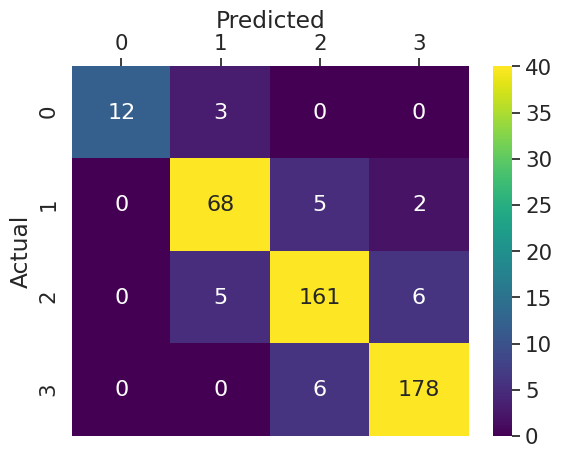
\includegraphics[width=0.45\textwidth]{templates/images/Figure-XGB16-ConfusionMatrix.png}
\singlespacing
\caption[XGBoost confusion matrix]{Confusion matrix for the tuned XGB model trained on WDS4.}
\label{fig:xgb_conf_matrix}
\end{wrapfigure}
A final XGB model parameterized with the tuned values was trained on the sixteen-feature version of WDS4. The resulting confusion matrix (Figure \ref{fig:xgb_conf_matrix}) demonstrates why XGBoost receives best-in-class praise as a predictive method. Test set accuracy for WDS4 exceeds 94\%. The largest number of misclassifications (12) occur between high-grade (class 3) and medium-grade (class 2) geothermal gradient. And ten additional inaccurate labels involve low-grade (class 1) mistaken as medium-grade or vice-versa. Only two records were off by more than one consecutive class. 

Figure \ref{fig:xgb_auc} shows the macro average, micro average, and individual class XGB ROC curves. All individual class AUC values are at or above 0.99. This is close to an ideal ROC plot for a classifier.

\begin{figure}[htp]
\centering
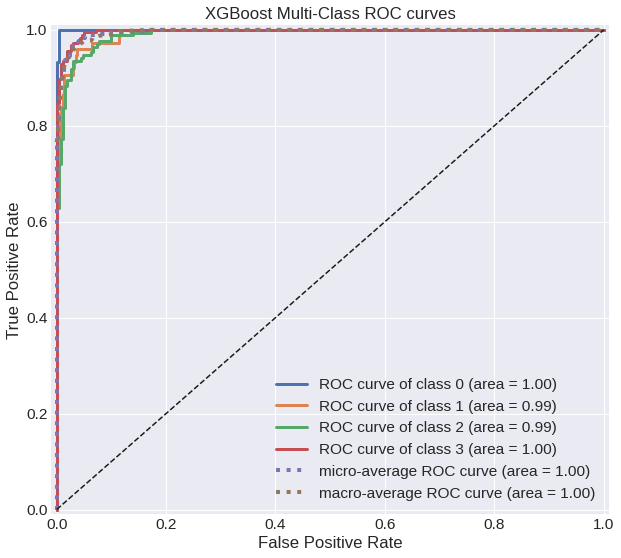
\includegraphics[width=.5\textwidth]{templates/images/Figure-XGB16-AUC.png}
\caption[XGBoost ROC curves]{ROC curves for tuned XGB model trained on WDS4.}
\label{fig:xgb_auc}
\end{figure}

Model predictions for the study area are generated by passing the FDS through the XGB model, as shown in Figure \ref{fig:xgb_final_map}. High-grade geothermal gradient areas to the southeast and central regions of the AOI align with the class 3 locations in the \citet{bielicki_hydrogeolgic_2015} PFA layer. The XGBoost model predicts more spatially continuous and connected high-grade regions, with a limited number of isolated patches to the southwest and on the northern section of the Rio Grande River. Both maps have a similar non-thermal class 0 region to the north, but they differ midway along the Rio Grande, to the south, and in the eastern panhandle where the PFA map predicts no-/low-grade classifications.

\begin{figure}[!htp]
\centering
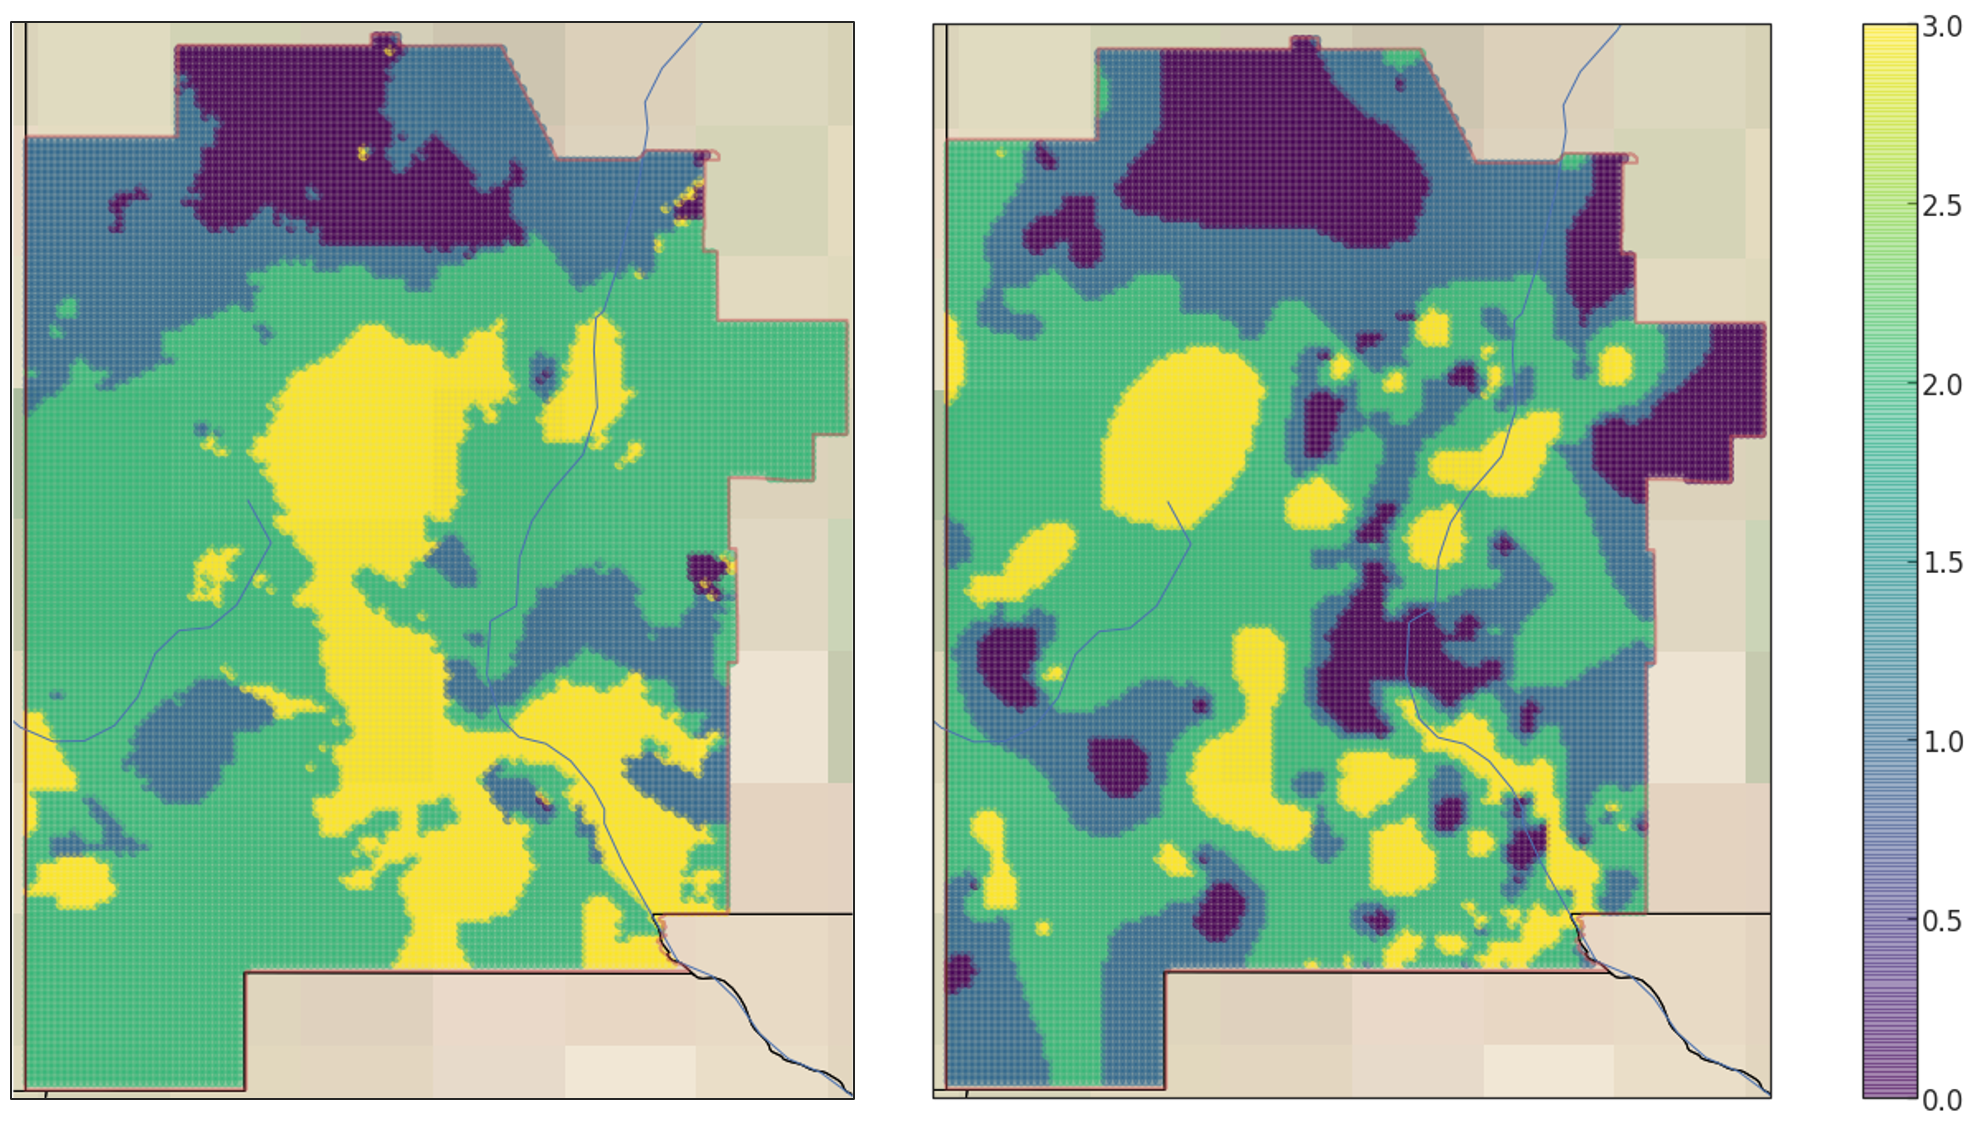
\includegraphics[width=\textwidth]{templates/images/Figure-XGB-FinalMap_Joint.png}
\caption[XGBoost prediction map]{Left: Map predictions of geothermal gradient from the tuned XGB model trained on WDS4. Right: geothermal gradient data layer from southwestern NM PFA study \protect\citep{bielicki_hydrogeolgic_2015}.}
\label{fig:xgb_final_map}
\end{figure}


%\section{Data Modeling}\label{ch5:modeling_overview}
%\begin{wrapfigure}{R}{0.45\textwidth}
%\centering
%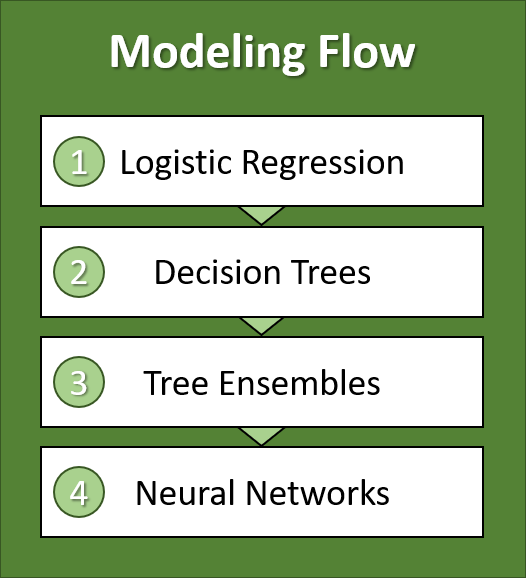
\includegraphics[width=.35\textwidth]{templates/images/Flow-Modeling.png}
%\singlespacing
%\caption[Modeling workflow]{Workflow for predicting the class of geothermal gradient across the southwestern NM study area using a variety of common machine learning methods.}
%\label{fig:model_flow}
%\end{wrapfigure}

%Supervised learning methods for classification come in a wide variety of shapes and sizes. Rather than settle on one for predicting geothermal gradient, four different methods are applied to the southwestern NM data set. Figure \ref{fig:model_flow} illustrates the high-level modeling flow, where model complexity increases with successive steps. The method descriptions below only briefly delve into important model mechanics and key hyperparameters (i.e., parameters not learned from data) that impact model performance. Other sources can provide a deeper review of machine learning algorithms and their mathematical underpinnings. This investigation should instead be considered an applied case study that uses these algorithms as tools for generating insights on geothermal potential.

%\subsection{Assessing Performance}\label{ch5:modeling_assessments}
%Building an intuition for the differences in predictive ability of different models first requires a clear definition of the scoring metric(s) used to compare those models. The characterization of classifier performance typically begins with a confusion matrix. In its simplest form, the confusion matrix evaluates class predictions as \acrlong{tp} (\acrshort{tp}; predicted 1, actually 1), \acrlong{tn} (\acrshort{tn}; predicted 0, actually 0), \acrlong{fp} (\acrshort{fp}; predicted 1, actually 0), and \acrlong{fn} (\acrshort{fn}; predicted 0, actually 1). For the multi-class problem, the confusion matrix expands to include all correct classification and misclassification options. Figure \ref{fig:confusion_matrix} illustrates the elements of a 4-class matrix.

%\begin{figure}[!htp]
%\centering
%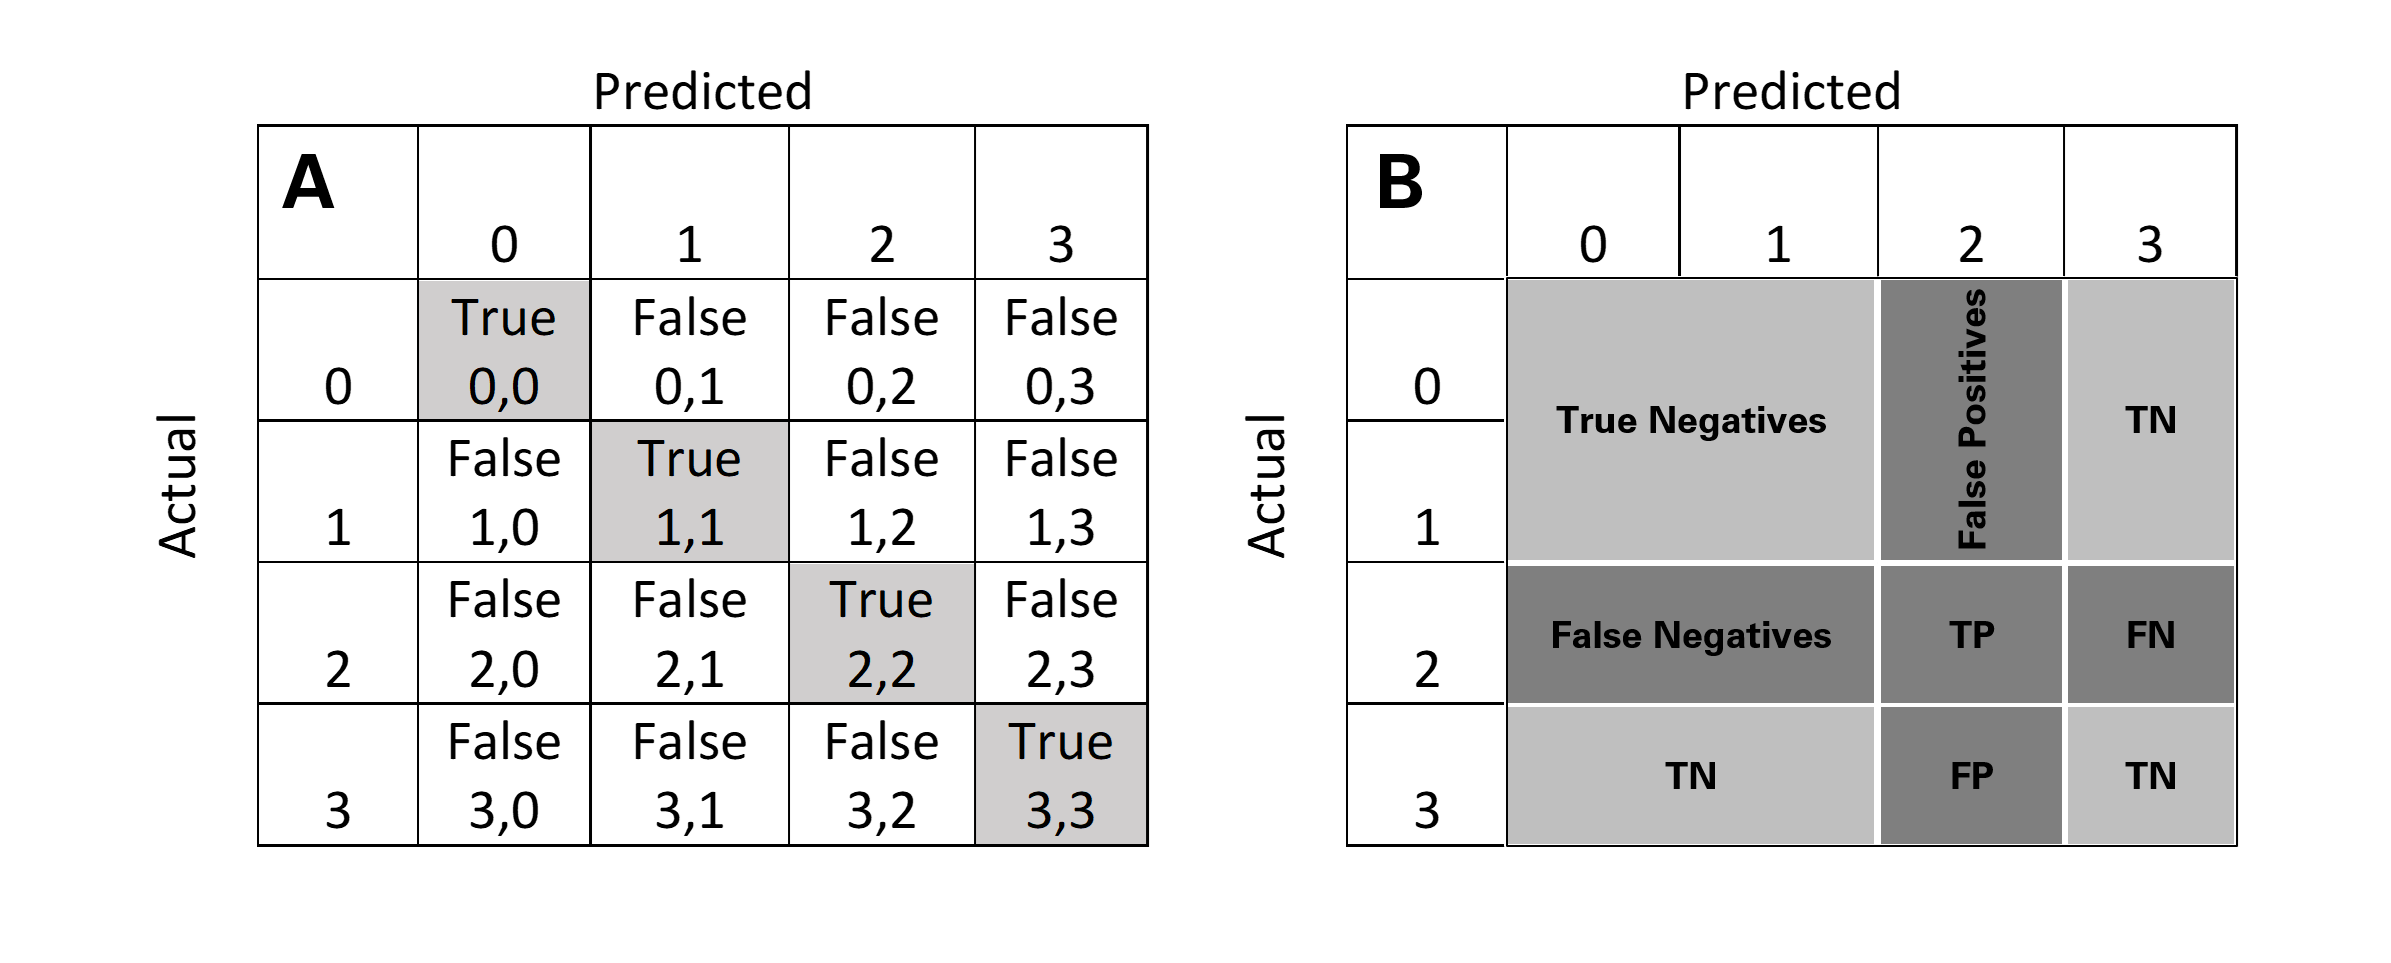
\includegraphics[width=\textwidth]{templates/images/Figure-Confusion_Matrix.png}
%\caption[Four-class confusion matrix]{Confusion matrix diagram for a 4-class scenario. A. Each cell represents a pairing between an actual class label (rows) and the predicted label (columns). True positives for each class are down the diagonal. B. Example of matrix interpretation using class 2 as a point of reference. Elements associated with TP, FP, TN, and FN values are labeled.}
%\label{fig:confusion_matrix}
%\end{figure}

%Several statistical measures can be defined using combinations of elements in the confusion matrix. Of significance to this study are the \acrlong{tpr} (\acrshort{tpr}) and \acrlong{fpr} (\acrshort{fpr}) \citep{tharwat_classification_2020}:

%\begin{itemize}[itemsep=2pt]
%\item \textbf{True Positive Rate}: the count of correctly-predicted positives scaled by the actual positives: TP/(TP$+$FN).
%\item \textbf{False Positive Rate}: the count of incorrectly-predicted positives scaled by the actual negatives: FP/(FP$+$TN).
%\end{itemize}

%Classification relies on a probability threshold for assigning a class label. As the threshold lowers, the chances the classifier will believe it has a label match will increase. By varying this threshold, it becomes possible to map out the discriminating ability of a classifier by plotting a curve in TPR vs. FPR space (Figure \ref{fig:roc}). This is commonly referred to as the \acrlong{roc} (\acrshort{roc}) curve \citep{fawcett_introduction_2006}. A classifier that cannot discriminate between classes will perform no better than random guessing, resulting in a curve that plots along the diagonal from the origin to the upper right of the plot. On the other hand, a perfect classifier will have a TPR of 1.0 for all thresholds, so it plots straight up along the y-axis and then horizontally at TPR = 1.0. Typical ROC curves plot in the upper-left space between these two extremes.

%\begin{figure}[!htp]
%\centering
%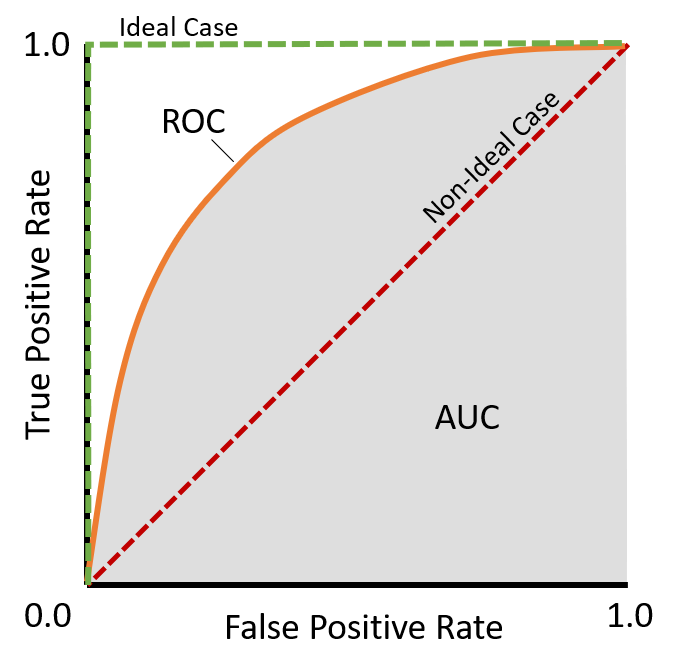
\includegraphics[width=0.5\textwidth]{templates/images/Figure-ROC_AUC_Diagram.png}
%\caption[Receiver Operating Characteristic diagram]{ROC curve diagram in TPR vs. FPR space. Perfect classifiers will plot along the ideal case line (green), poor classifiers plot along the diagonal (red). AUC (gray) characterizes the quality of the classifier on a scale of 0.5 to 1.0.}
%\label{fig:roc}
%\end{figure}

%Area Under the ROC Curve (AUC) defines a summary statistic for the ROC function (see Figure \ref{fig:roc}) \citep{fawcett_introduction_2006}. Since the ideal classifier has a TPR of 1.0 at all times, the ideal AUC also equals 1.0. In the non-ideal case, the AUC drops to 0.5. AUC values and ROC curves provide a standardized means of comparing classifiers and are the primary performance metric used in this thesis.

%With multi-class classification, defining single class performance using the definitions of TP, FP, TN, and FN as shown in Figure \ref{fig:confusion_matrix}B is relatively straight-forward. Overall classifier performance across all classes can also be characterized with a single ROC curve using macro, weighted, or micro averaging \citep{scikit-learn_sklearnmetricsroc_auc_score_2021}.

%\begin{itemize}[itemsep=2pt]
%    \item \textbf{Macro}: averaging matches the unweighted arithmetic mean of metric values.
%    \item \textbf{Weighted}: averaging follows the procedure of macro-averaging but adds a weight for each class contribution based on the fraction of total observations that fall within that class. 
%    \item \textbf{Micro}: averaging considers class results in aggregate, so statistics are calculated across the entire confusion matrix. TPR becomes the accuracy and FPR becomes the error rate.
%\end{itemize}

%For imbalanced data sets, micro will indicate better performance than macro due to the impact of the dominant class. Both micro and macro averages are included in the classification analysis in the following sections.

%\subsection{Logistic Regression} \label{ch5:logistic_regression}
%\subsubsection{Binary Formulation} \label{ch5:lr_math}
%The classic \acrlong{lr} (\acrshort{lr}) model is a binary classifier that predicts one of two labels based on the input data. Linear regression treats the problem as a linear combination of the input observations \citep[p.\ 369]{bertsimas_analytics_2016}:

%\begin{equation}
%\label{eq:linreg_form}
%    \hat{y} = {\bf{w^Tx}} = w_0 + w_1 \cdot x_1 + w_2 \cdot x_2 + \ldots + w_n \cdot x_n 
%\end{equation}

%Where $x_i$ are the feature observations, $w_i$ are coefficients or weights for those features, and $\hat{y}$ is the weighted sum. Logistic regression adjusts the problem such that predictions define the probability of belonging to class 1. This is done by using a non-linear logistic response function: 

%\begin{equation}
%\label{eq:sigmoid}
%h_{\theta}(x) = \frac{1}{(1+e^{-\hat{y}})} = %\frac{1}{(1+e^{-W^TX})}
%\end{equation}

%Equation \ref{eq:sigmoid}, also known as the \textit{sigmoid} function, converts the weighted sum from equation \ref{eq:linreg_form} to values between 0 and 1 \citep[p.\ 369]{bertsimas_analytics_2016}. Solving for the weights in this equation ($w_i$) requires an iterative optimization procedure like gradient descent. This procedure minimizes a cost function ($J(\Theta)$) based on the negative log likelihood \citep{ng_logistic_2011}:

%\begin{equation}
%\label{eq:logreg_cost}
%\begin{aligned}
%        J(\Theta) &= -\frac{1}{m} \sum_{i=1}^{m}{\text{Cost}(h_{\theta}(x_i),y_i)} \\ &= -\frac{1}{m}\sum_{i=1}^{m}{(y_i*\text{log}({h_{\theta}(x_i)})+(1-y_i)*\text{log}(1-h_{\theta}(x_i)))}
%\end{aligned}
%\end{equation}

%Regularization is added to logistic regression to avoid overfitting, specifically by penalizing the sum of the squared weights (L2-regularization). A constant ($\lambda$) determines the trade-off of influence between the magnitude of the weights and negative log likelihood in the minimization \citep{ng_regularization_2011}.

%\begin{equation}
%\label{eq:logreg_cost_reg}
%    regularized\,J(\Theta) = -\frac{1}{m}\sum_{i=1}^{m}{\text{Cost}(h_{\theta}(x_i),y_i) + \frac{\lambda}{2m}\sum_{j=1}^{n}{w_j^2}}
%\end{equation}

%The scikit-learn \textit{LogisticRegression} function uses a constant C applied to the negative log likelihood term, which acts like the inverse of $\lambda$. Larger values of C result in less regularization \citep{scikit-learn_1111_2021}.

%\subsubsection{Multi-Class Heuristics} \label{ch5:lr_multiclass}
%This formulation of logistic regression defines a strictly binary classification problem without multi-class support. Two heuristic methods allow LR to extend to multi-class classification: \acrlong{ovo} (\acrshort{ovo}) and \acrlong{ovr} (\acrshort{ovr}) \citep{brownlee_one-vs-rest_2020,scikit-learn_multiclass_2021}. Both split the problem into multiple binary classifications. OvO considers every class versus every other class. In the 4-class geothermal gradient problem, this amounts to six classifications: {(0 vs. 1), (0 vs. 2), (0 vs. 3), (1 vs. 2), (1 vs. 3), (2 vs. 3)}. OvR simplifies the problem by combining class alternatives so the number of classifiers matches the number of classes: {(0 vs. [1, 2, or 3]),(1 vs. [0, 2, or 3]), (2 vs. [0, 1, or 3]),(3 vs. [0, 1, or 2])}. For both methods, the class with the greatest score or sum of scores wins, where the score is akin to the probability of class membership. This thesis uses the OvR strategy.

%\subsubsection{Stratified k-Fold Cross-Validation} %\label{ch5:strat_kfold_cv}
%Brute force tuning of a hyperparameter can be accomplished by training a series of classifiers with different hyperparameter values and evaluating each classifier's predictive ability against the validation data subset. A more statistically stable approach involves k-Fold \acrlong{cv} (\acrshort{cv}). K-fold CV splits the input data into a number of subsets, or folds. It trains the model on the aggregate of all but one fold, then scores the classifier based on that remaining fold \citep[p. 181]{james_introduction_2013}. This leave-one-fold-out strategy cycles through all k permutations, and the scores are averaged to produce a summary statistic --- in this case, the AUC. For imbalanced class data, folds can be stratified sampled such that class proportions are preserved within each fold \citep{brownlee_how_2020}. For parameter tuning, the k-Fold CV will define a set of average scores for the range of hyperparameter values under consideration, and the optimal parameter value can be determined from a plot of those scores.

%\subsubsection{Feature Selection} \label{ch5:lr_rfe}
%By consequence of Equation \ref{eq:sigmoid}, logistic regression assumes a linear relationship between the weighted sum of independent predictors and the log-odds, i.e., $\log(\frac{P(y=1)}{1-P(y=1)})$. However, including all possible predictors will not necessarily improve the model. Feature selection can lead to simpler models with the same predictive power but reduced risk of collinearity, which is important when managing data from naturally integrated earth systems. 

%One method for selecting the features to keep involves an iterative process called \acrlong{rfe} (\acrshort{rfe}) (Brownlee, 2020c; scikit-learn, 2021d). The concept is relatively simple: RFE recursively selects and removes the feature with the smallest coefficient in the logistic regression model, then refits the data and repeats until a user-defined number of features is reached.  A plot of AUC vs. number of features can be constructed by looping over different feature limits, where the logistic regression model is fit on the training subset and evaluated on the validation subset 

%\subsubsection{Optimized Model Results}\label{ch5:lr_results}

%\subsection{Decision Trees}\label{ch5:decision_trees}
 
%A decision tree, sometimes known as a Classification and Regression Tree (CART), classifies observations using a cascading set of evaluations, each on individual predictor variables. There is no assumption of a linear response in the system. In fact, decision trees are uniquely suited to representing non-linear behavior in a highly-explainable way; once constructed, the decision tree describes a flowchart-like roadmap for each label assignment \citep[p. 373--375]{bertsimas_analytics_2016}. Not every predictor will necessarily appear in the decision tree --- only those found to be significant during tree construction. And the most significant variables tend to be associated with early decision splits, placing them higher in the tree \citep[p. 376]{bertsimas_analytics_2016}. Because of this, decision trees naturally provide insights into feature importance. 

%\subsubsection{Tree Construction}
%Decision trees are constructed by recursively performing binary splits on the training data set. Each split defines two new nodes in the tree, which correspondingly separates a group within the training data into subgroups. These subgroups represent child paths from the split node that terminate in two new terminal leaf nodes on the tree. The classification decision for each leaf will be the most commonly occurring class from the training data observations that are assigned to that leaf \citep[p. 311]{james_introduction_2013}.

%There are three metrics that can play a role in evaluating the discriminating quality of a particular decision node on the tree:

%\begin{itemize}[itemsep=2pt]\label{ch5:impurity}
%    \item \textbf{Classification error rate}: the proportion of training samples that do not match the dominant class associated with a leaf node \citep[p. 312]{james_introduction_2013}.
%    \begin{equation}
%    \label{eq:error_rate}
%        E = 1 - \max_k(\hat{p}_{mk})
%    \end{equation}
%    where $m$ is the segment of the data associated with a node, $k$ is the class, and $\hat{p}_{mk}$ is the fraction of all training observations in $m$ that are of class $k$. 
%    \item \textbf{Gini index}: measures variance across all k classes. Gini is sometimes known as a purity measurement because low values correspond with a strongly dominant class \citep[p. 312]{james_introduction_2013}.
%    \begin{equation}
%    \label{eq:gini}
%        G = \sum_{k=1}^{K}{\hat{p}_{mk}(1-\hat{p}_{mk})}
%    \end{equation}
%    \item \textbf{Entropy}: An alternative form of purity measure, which also shows low values when the proportion of one class dominates the others within a node \citep[p. 312]{james_introduction_2013}.
%    \begin{equation}
%    \label{eq:entropy}
%        D = -\sum_{k=1}^{K}{\hat{p}_{mk}* \text{log}(\hat{p}_{mk})}
%    \end{equation}
%\end{itemize}

%The purity aspect of both Gini index and entropy make them good choices for tree construction. In the forward pass, the tree will iteratively grow by selecting nodes in the tree, a predictor to split on, and a threshold value defining the split. These choices are optimized by the chosen quality metric. The tree will grow until a stopping condition is met, like reaching a maximum tree depth or minimum number of observations allowed per node. Tree clean-up then takes place in a backward pass, where the following decision tree objective governs whether a tree branch is kept or removed \citep[p. 309]{james_introduction_2013}:

%\begin{equation}
%\label{dtree_objective}
%\begin{aligned}
%    J(\Theta) &= SSE + \alpha\left|T\right| \\
%    &= \sum_{m=1}^{\left|T\right|}{\sum_{i|x_i\epsilon R_m}}{(y_i-\hat{y}_m)^2+\alpha\left|T\right|}
%\end{aligned}
%\end{equation}

%Here, $\left|T\right|$ refers to the number of terminal nodes in tree $T$, $R_m$ is the subgroup of the training data associated with terminal node $m$, and $\hat{y}_m$ is the classification predicted by node $m$. If the sum of squared errors ($SSE$) in classification increases by less than $\alpha$ when a branch is removed, that branch will remain removed from the decision tree. $\alpha$ acts as a regularization parameter balancing prediction accuracy with model complexity; greater values of $\alpha$ result in simpler decision trees.

%\subsubsection{Hyperparameter Tuning} \label{ch5:dtree_tuning}

%\subsubsection{Feature Selection} \label{ch5:dtree_feat_importance}

%\subsubsection{Optimized Model Results}

%\subsection{Tree Ensembles (XGBoost)}

%As simple and effective as decision tree classifiers may be, they only demonstrate a single model solution. And since random selection can play a role in their construction, completely different tree structures may arise if a tree is rebuilt on the same data set. The random forest algorithm embraces these random variations and generates a large number of decision trees. To increase randomness, only a subset of the predictors are used when building each tree, and the trees are trained on a different data subset selected at random and with replacement from the full training set \citep[p. 376--377]{bertsimas_analytics_2016}. Much like the classic “wisdom of crowds” paradigm, the collection of trees acts as a single, more performant ensemble model. However, greater possible accuracy in predictions from the ensemble trades off with less interpretability; as the forest grows larger, the number of constituent decision trees quickly exceeds the limits of human comprehension. As such, ensemble tree methods like random forests are considered black box algorithms.

%A variation in ensemble algorithms uses “gradient boosting,” where the trees in the ensemble are chained in succession and train on the residual error of the preceding tree. The trees are weak learners that underfit the data, giving them low variance, but high bias. Yet when the predictions of the models are summed together, the compound prediction can out-perform more conventional random forests \citep[p. 323]{james_introduction_2013}:

%\begin{equation}
%\label{eq:xgb_form}
%    \hat{f}(x) = \sum_{b=1}^{B}{\alpha \hat{f}^{b}(x)}
%\end{equation}

%Where $\hat{f}(x)$ is the boosted model, $\hat{f}^b$ are the weak learners totaling $B$ in number. $\alpha$ is the shrinkage parameter or learning rate. 

%XGBoost is a variant of gradient-boosting tree algorithms, gaining a significant amount of notoriety from machine learning competition wins \citep{chen_dmlcxgboost_2021}. The objective function governing model construction balances two influences \citep{chen_xgboost_2016}:

%\begin{equation}
%\label{eq:xgb_objective}
%\begin{aligned}
%    J(\Theta) &= L + \Omega \\
%    &= \sum_{i}{l(\hat{y}_i,y_i)}+\sum_{k}{\Omega(f_k)} \\
%    &= \sum_{i}{l(\hat{y}_i,y_i)}+\sum_{k}{\left({\gamma T}+\frac{1}{2} \lambda \sum_{j=1}^T{w_j^2}\right)}
%\end{aligned}
%\end{equation}

%Where the first part expresses how well the model fits the data (i.e., the loss), while the second term regulates the complexity of the model. Complexity is defined by the number of leaves in a tree ($T$) and the size of leaf weights ($w$) unique to XGBoost decision trees. After some additional derivations, the objective can be restated as: 

%\begin{equation}
%\label{eq:xgb_obj_simple}
%    J(\Theta) = -\frac{1}{2}\sum_{j\;leaves}{\frac{G_j^2}{H_j + \lambda} + \gamma T}
%\end{equation}

%Where $G$ is the sum of the first-order gradient statistics for the instance set of leaf $j$, and $H$ is the sum of the second-order gradient statistics \citep{chen_xgboost_2016}. Tree construction follows that of decision trees --- split each node greedily to maximize tree depth, then prune back in a backward pass. The left term of equation \ref{eq:xgb_obj_simple} provides a means to calculate loss reduction for a candidate split, thus governing the evaluation of tree splits during the pruning process. 

%XGBoost is a complex algorithm, but with a lot of optimizations that make it extremely efficient, scalable, and popular among machine learning practitioners.

%\subsubsection{Hyperparameter Tuning}

%\subsubsection{Feature Selection}\label{ch5:xgb_shapley}

%As a tree-based machine learning method, XGBoost naturally provides feature importances as a product of model-fitting. The XGBoost package offers five kinds of global feature importance calculations \citep{xgboost_developers_xgboost_2020}, but each may give a slightly different ordering and suggested relative impact of the predictors in the feature set. At issue here are two concepts in importance definition methods: consistency, or the independence of a feature importance value and the reliance of a model on that feature, and local accuracy, or the idea that the sum of the importances is equivalent with the overall model importance \citep{lundberg_interpretable_2020}. A study of six different approaches to interpreting models through feature attribution showed most do not meet both desirable properties, with the exception of \acrlong{shap} (\acrshort{shap}) values \citep{lundberg_consistent_2019}.


%Shapley values derive from cooperative gain theory \citep{shapley_value_1997}, but have gained traction in the machine learning community partly because they predict importances without assuming complete feature independence \citep{lundberg_unified_2017}. In addition to managing collinearity, Shapley values have several desirable features. For example, if two features impact a model prediction equally, they will also have equivalent Shapley values. And a Shapley value of zero means the feature has no predictive impact. The SHAP method produces values that have global significance for general feature importance but also local significance for an individual prediction; the sum of SHAP values is equivalent to the deviation of the model prediction from the average value (baseline), meaning SHAP values describe the individual contributions of each feature to a prediction value \citep{lundberg_unified_2017}.

%\subsubsection{Optimized Model Results}\label{ch5:xgb_final_model}

\section{Neural Networks} \label{ch5:ann_model}
%\subsection{Neural Networks} \label{ch5:ann}

%\subsubsection{Model Concept}
%\label{ch5:ann_concept}

%The original concepts behind Artificial Neural Networks (ANNs or just \acrshort{nn}s) come from simplified models of neuron activity in the brain \citep[p.\ 394]{hastie_elements_2009}. At a high level, multiple inputs are fed into neuron cells from many branches on one end, and given the right combination of those inputs, these cells will fire and propagate a signal to the next group of connected neurons.

%In neural networks, cells are represented by logistic units (Figure \ref{fig:nn_schematic}). Each unit acts like a logistic regression operation, where inputs are scaled by weights, and the linear sum of the weighted inputs are passed through an “activation function” to determine if the output is a 0 or a 1. As in logistic regression, the sigmoid function (Equation \ref{eq:sigmoid}) commonly appears in network architectures, but many additional activation functions like the \acrlong{relu} (\acrshort{relu}) are frequently used as well \citep{brownlee_gentle_2019}.

%\begin{figure}[!htp]
%\centering
%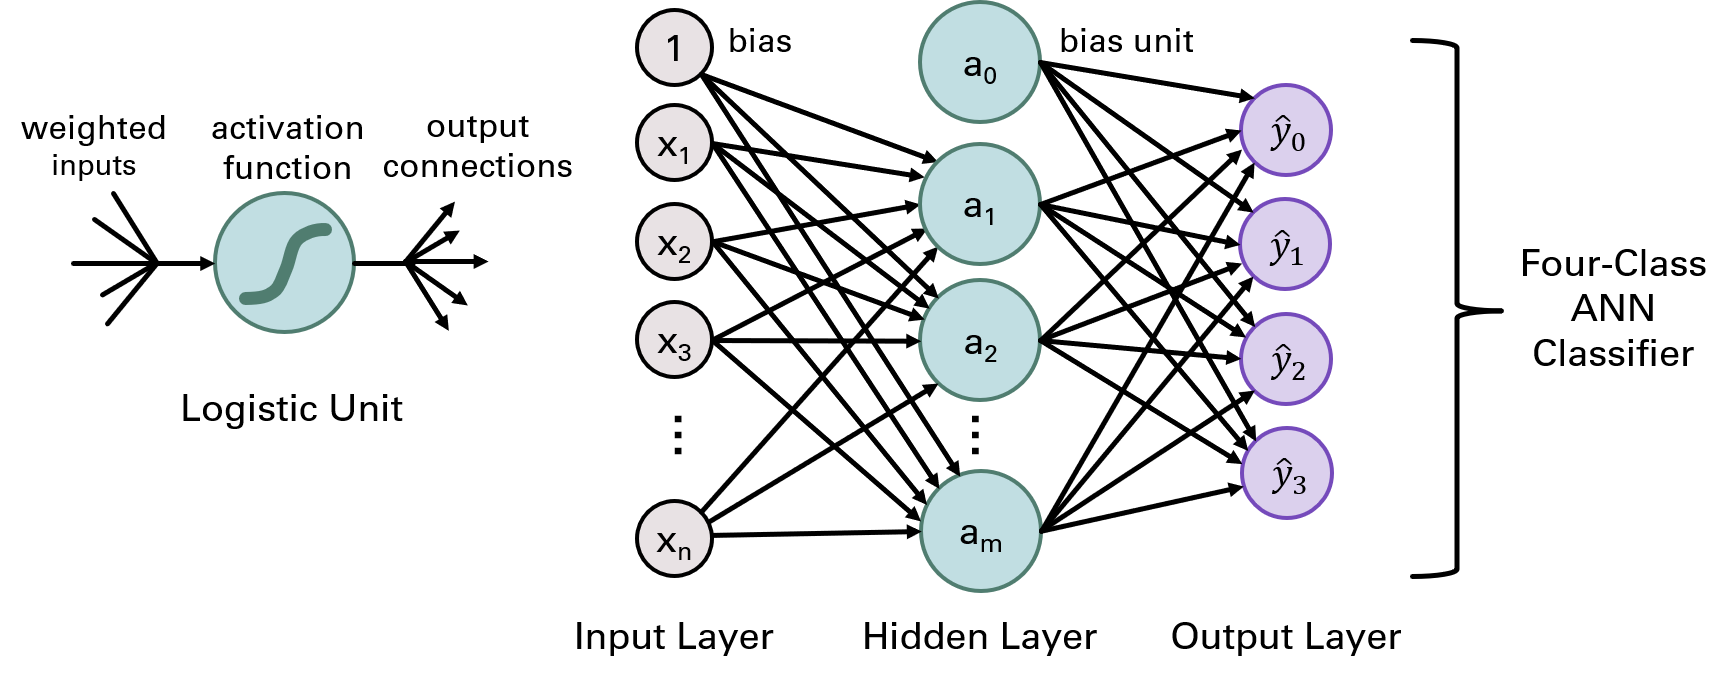
\includegraphics[width=\textwidth]{templates/images/Figure-ANN.png}
%\caption[Neural network schematic]{Schematic of a logistic unit (Left) and a fully-connected neural network (Right) with a single hidden layer made up of logistic units $a_1$ through $a_m$. Bias units (subscript 0) traditionally have a value of 1, but are weighted in linear combinations like other units. Four units in the output layer make this a four-class classifier.}
%\label{fig:nn_schematic}
%\end{figure}

%Each logistic unit performs the following operation:

%\begin{equation}
%\label{eq:nn_activation}
%    {\bf{a}} = g({\bf{z}}) = g({\bf{W^TX}})
%\end{equation}
%\\
%where $g$ is the activation function and $\bf{W}$ are the weights. For the first hidden layer, $\bf{X}$ will be the predictor values from the input layer as shown in Figure \ref{fig:nn_schematic}. For any additional hidden layers, $\bf{X}$ consists of the outputs of units from the preceding layer. Here, $\bf{z}$ is described in matrix notation but has the same form as Equation \ref{eq:linreg_form}. 

%The cost function for a neural network takes on the form of a loss term and a complexity term \citep{ng_neural_2011}:

%\begin{equation}
%\label{eq:nn_cost_function}
%    \begin{aligned}
%        J(\Theta) &= 
%        -\frac{1}{m}\sum_{i=1}^{m}{
%        L(\hat{y}_i, y_i)} + \frac{\lambda}{2m}
%        \sum_{l=1}^{L-1}{
%        \sum_{i=1}^{s_l}{
%        \sum_{j=1}^{s_{l+1}}{(w_{ij}^{l})^2}}} \\
%        &= -\frac{1}{m}
%        \sum_{i=1}^{m}{
%        \sum_{k=1}^{K}{
%        y_k^{(i)}\log{h_{\theta}(x^{(i)})_k}+
%        (1-y_k^{(i)})\log{(1-h_{\theta}(x^{(i)})_k)}}}\ + \\
%        &\qquad \frac{\lambda}{2m}
%        \sum_{l=1}^{L-1}{
%        \sum_{i=1}^{s_l}{
%        \sum_{j=1}^{s_{l+1}}{(w_{ij}^{l})^2}}}
%    \end{aligned}
%\end{equation}

%Which looks very similar to the regularized negative log likelihood cost function for logistic regression (Equation \ref{eq:logreg_cost_reg}). Here, $m$ is the number of predictor values in the input layer, $K$ is the number of outputs, $L$ is the number of layers, and $i$ and $j$ track the weights for layer $j$, unit $i$. $\lambda$ is a regularization term controlling the balance between the loss term and complexity term in the cost function. 

%As usual, minimizing this loss function is the goal of the NN learning process. This is generally accomplished using the backpropagation algorithm to compute the gradients needed for a gradient descent optimization \citep[p.\ 396]{hastie_elements_2009}.

\subsubsection{Network Architecture}
\label{ch5:ann_structure}

\begin{figure}[!htp]
\centering
\begin{minipage}[b][][b]{.35\linewidth}
    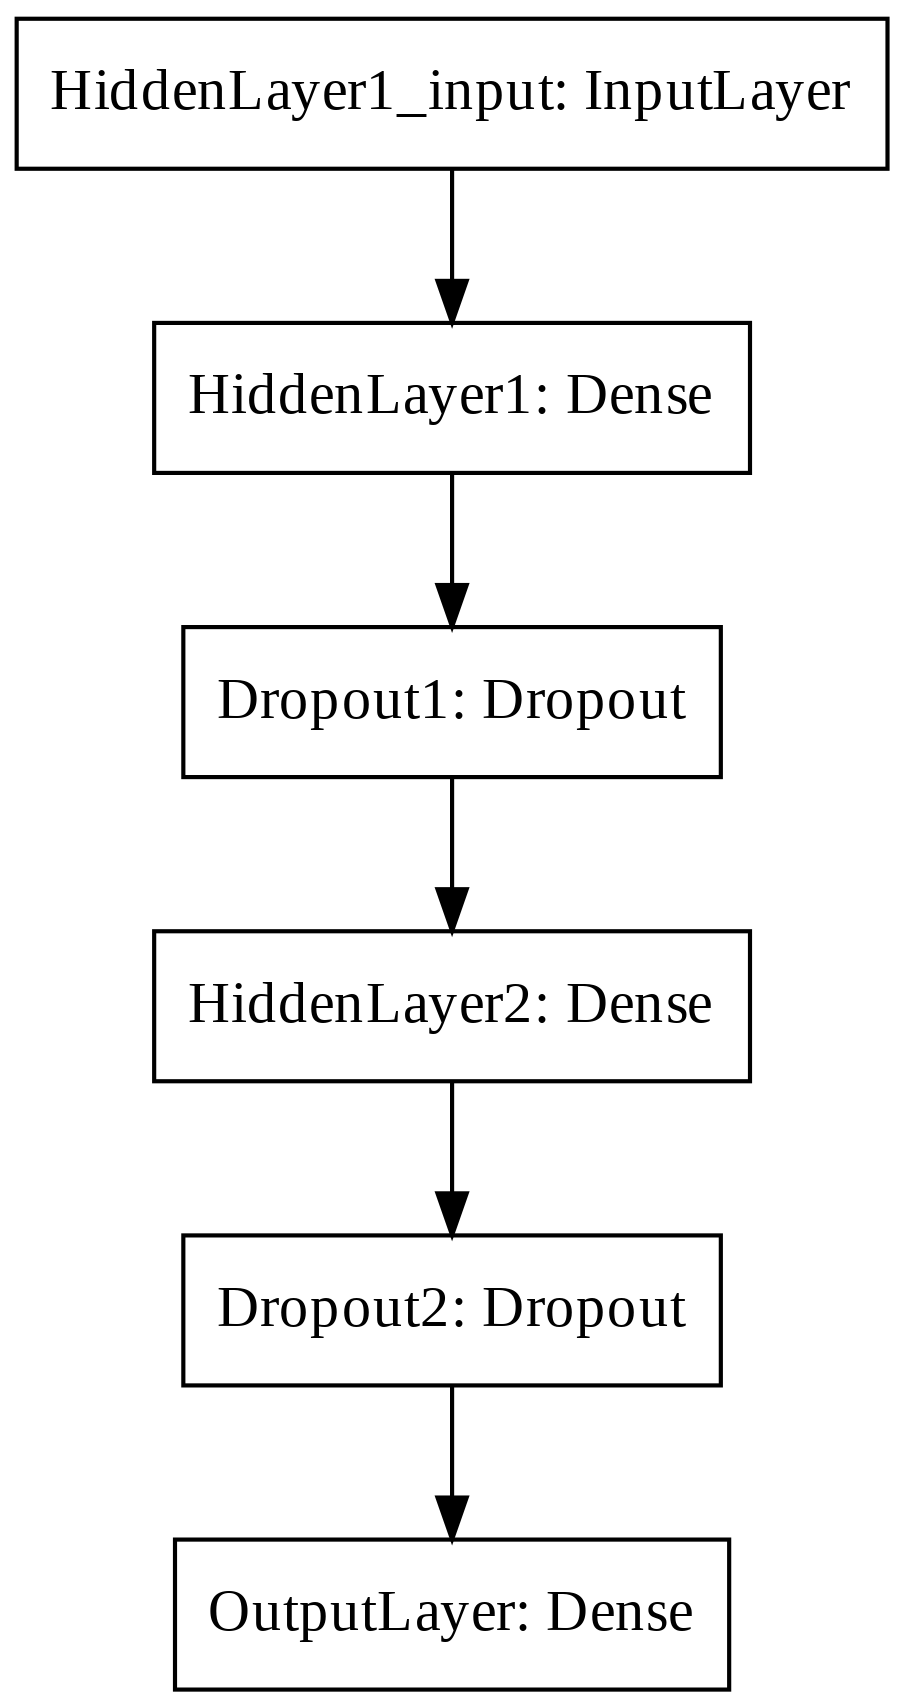
\includegraphics[width=\linewidth]{templates/images/Figure-TF_NN_Structure.png}
    \caption[Neural network structural flow]{Structural flow chart for the TensorFlow-based neural network.}
    \label{fig:nn_text_structure}
\end{minipage}
\hfill
\begin{minipage}[b][][b]{.61\linewidth}
    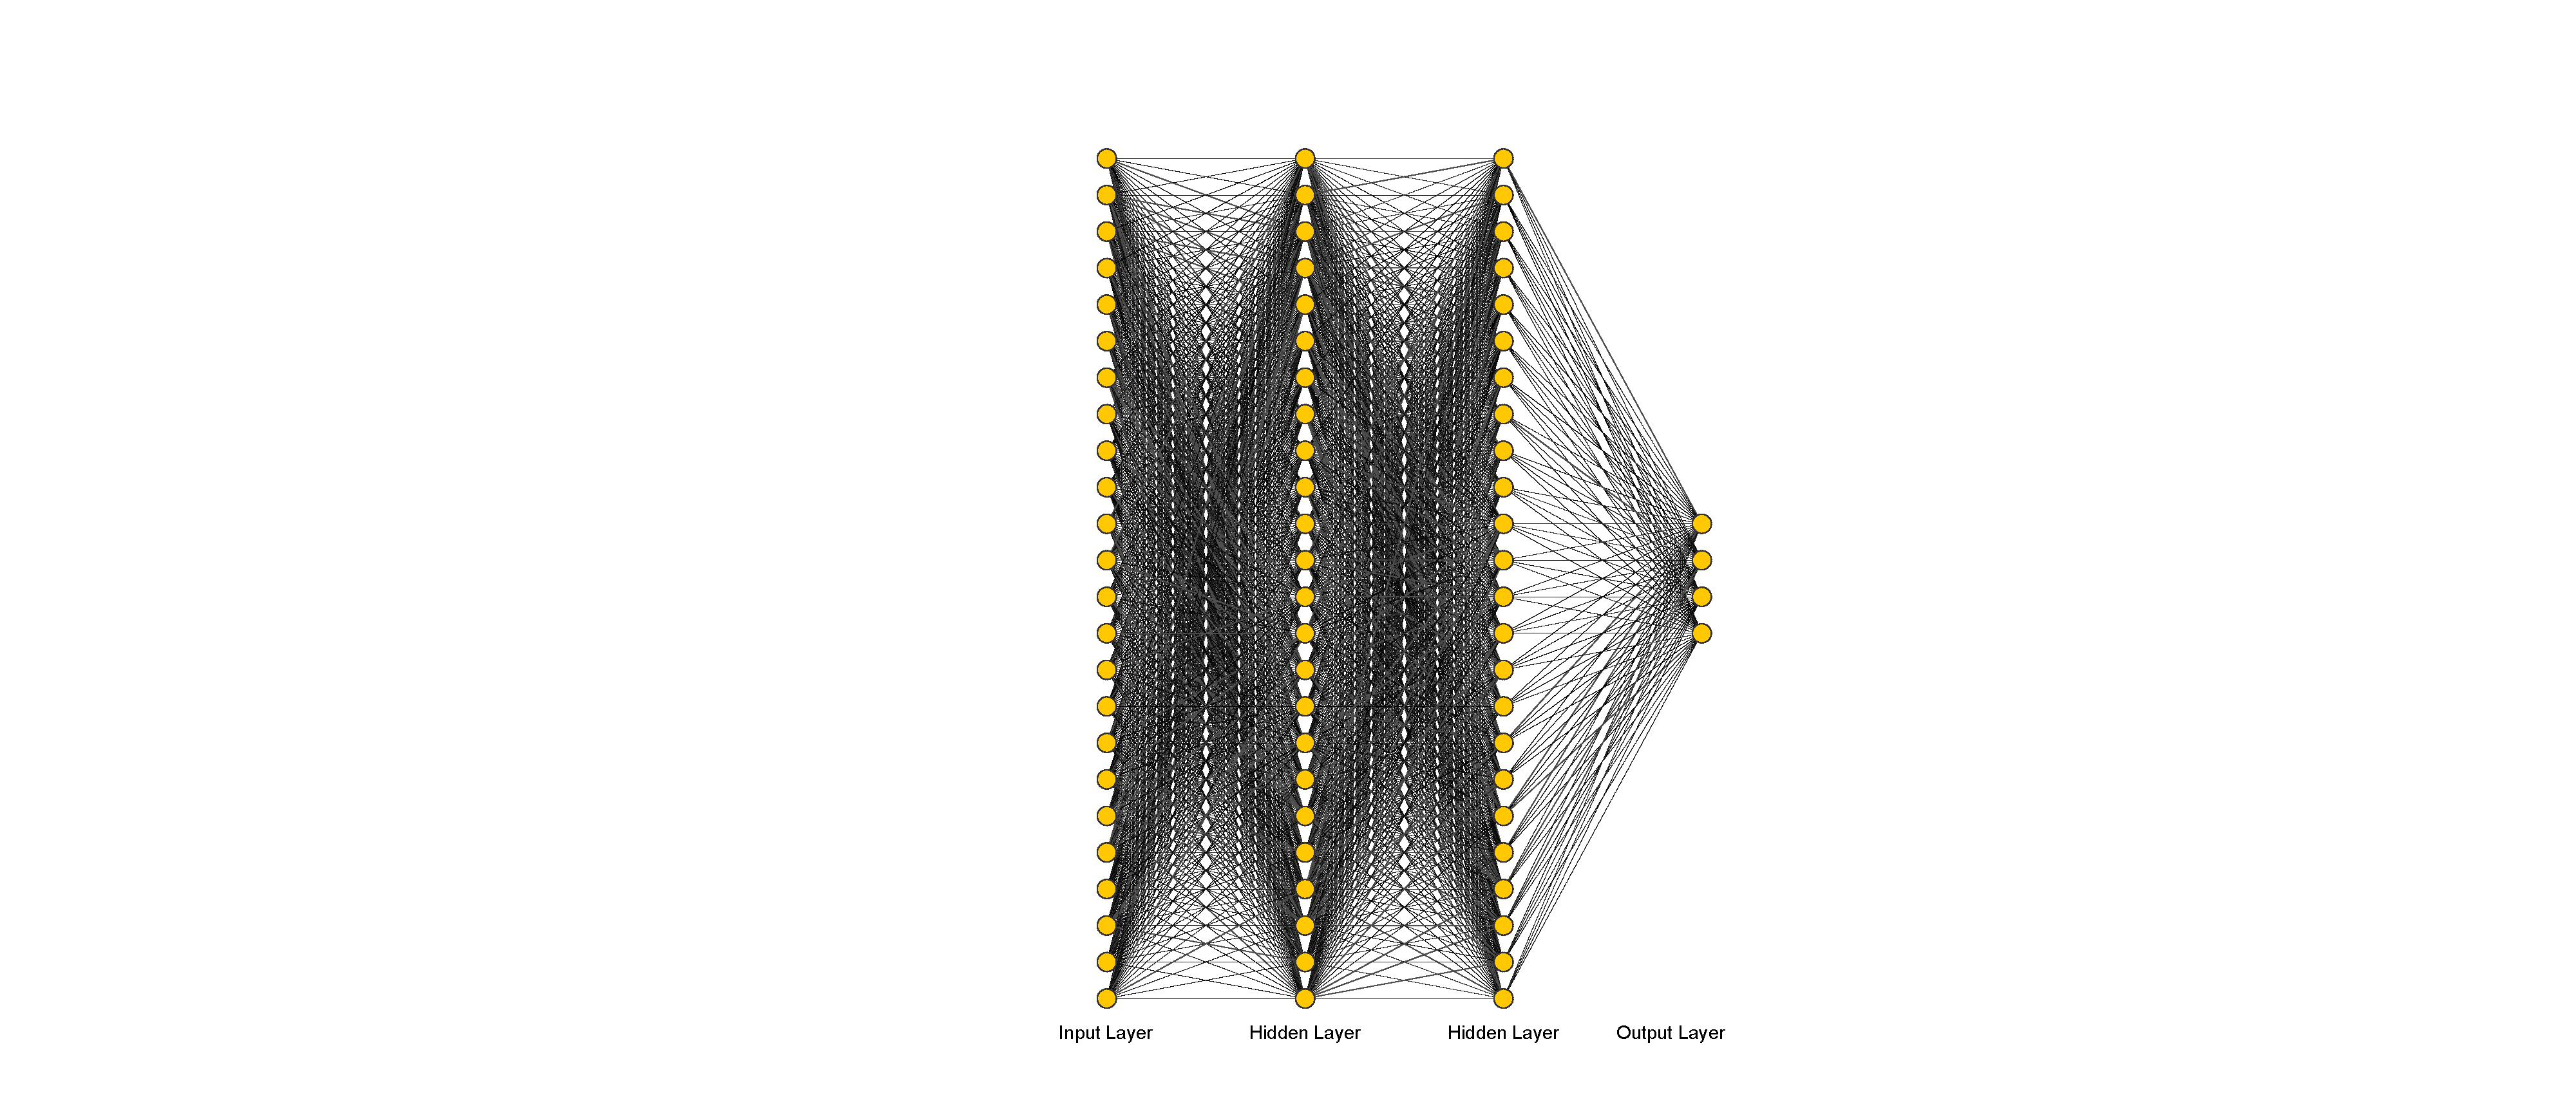
\includegraphics[width=\linewidth]{templates/images/Figure-ANN.pdf}
    \caption[Neural network structural schematic]{Schematic diagram of the neural network. Not shown are the dropout operations after each hidden layer.}
    \label{fig:nn_dot_structure}
\end{minipage}
\end{figure}

This thesis uses a TensorFlow-constructed neural network to test geothermal gradient classification performance for the southwestern NM study area \citep{abadi_tensorflow_2016}. The network design is a 4-layer structure starting with an input layer of size (1x24), followed by two hidden layers sized (1x24), and ending in a four-class output layer (1x4) (Figures \ref{fig:nn_text_structure}, \ref{fig:nn_dot_structure}). Layer sizes assume all 24 features are included in the training. In addition, the network applies dropout after each of the hidden layers. Dropout helps prevent overfitting by randomly assigning inputs to zero, temporarily severing a defined percentage of node connections during each step of the training process.

Since the number of weights being learned scales with the layer count and size of each layer, the choice of network architecture is a tunable parameter. The simplicity of this \acrlong{fcn} (\acrshort{fcn}) design keeps the architecture easily explainable while still enabling the network to learn complex non-linear relationships for geothermal gradient prediction.

Likewise, the choice of activation functions for each layer may also impact the performance of the network. ReLU functions overcome several limitations seen with more traditional activation choices like the sigmoid function, e.g., limited sensitivity and vanishing gradients, making ReLU the present-day default standard for neural networks \citep{brownlee_gentle_2019}. Both hidden layers in the network described here apply ReLU activation functions.

The Adam optimization method was chosen for training the network due to its computational efficiency and current status as the recommended general-purpose optimizer \citep{brownlee_gentle_2017}. A description of Adam is beyond the scope of this thesis, but more information is widely available elsewhere \citep[e.g.,\ ][]{kingma_adam_2017}.

The training process updates network weights using gradients calculated from the entire training data in each training epoch \citep[p.\ 397]{hastie_elements_2009}. Successive epochs adjust the NN to match the training data even more, so evaluating loss, AUC, or other metrics on both the training and validation sets is important for identifying the best number of epochs to avoid overfitting. Training can also proceed with mini-batches, that is, small subsets of the training set, rather than the whole set at once. This method makes the training results noisier, but generally speeds up learning while adding a regularization effect to changes in the weights \citep{brownlee_how_2019}.  

\subsubsection{Hyperparameter Tuning}
\label{ch5:ann_tuning}

Parameter tuning therefore focuses on five hyperparameters:
\begin{itemize}[itemsep=2pt]
    \item \textbf{Learning rate}: scales the size of the updates to weights during each step of the training process. The Adam optimizer adjusts this rate during training, so the value here defines a starting learning rate. Initially set to 0.001.
    \item \textbf{Lambda ($\lambda$)}: the L2 weight regularization term, i.e., the $\lambda$ in equation \ref{eq:nn_cost_function}. Initially set to $1\times10^{-4}$.
    \item \textbf{Batch size}: the number of training samples included in each mini-batch when calculating training gradients for updating the network weights. Initially set to number of samples/10.
    \item \textbf{Dropout rate}: the fraction of network connections zeroed-out during each step of the training process. Initially set to 0.2.
    \item \textbf{Number of epochs}: the number of training repetitions when fitting the model to the data. Initially set to 100.
\end{itemize}

\begin{figure}[htp]
\centering
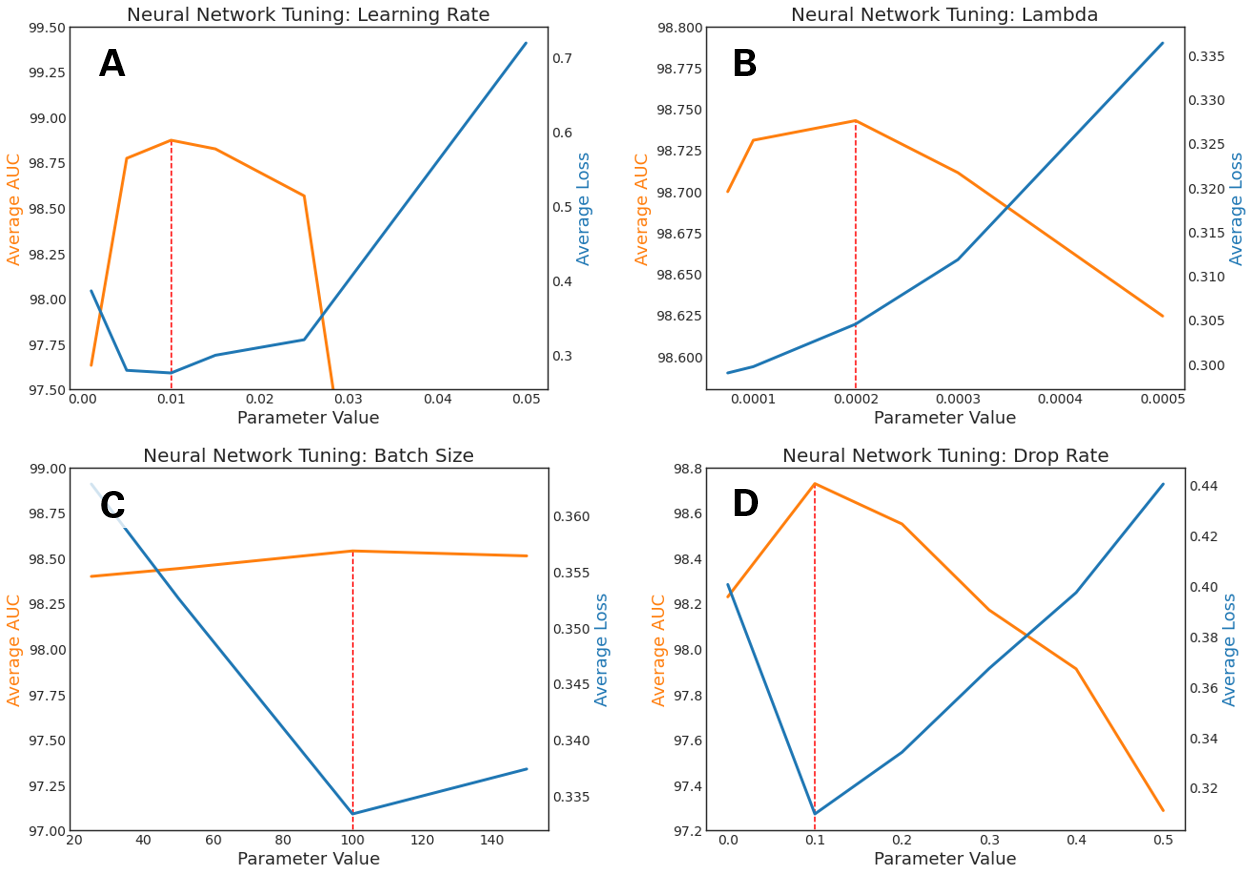
\includegraphics[width=\textwidth]{templates/images/Figure-NN_Hyperparameters.png}
\caption[Neural network hyperparameter tuning]{NN hyperparameter tuning results for A. learning rate, B. lambda ($\lambda$), C. batch size, D. and drop rate, using WDS4. The orange lines track AUC after 100 training epochs, averaged over 10-folds of stratified cross-validation for each parameter value. The blue lines show average loss after 100 epochs. Red dashed lines mark the selected values for the final model.}
\label{fig:nn_tuning_plots}
\end{figure}

The stratified k-fold cross-validation strategy described in Section \ref{ch3:strat_kfold_cv} was used for tuning NN hyperparameters. Training continued for 100 epochs, and since TensorFlow models easily track metric values for both the training and validation sets at each epoch, the two sets were kept separate during the 10-fold CV process. In the figures and discussion that follow, results are described for WDS4. Full results for all three data sets are provided in Table \ref{tab:nn_tuning}. 

%\begin{wraptable}{R}{0.50\linewidth}
\begin{table}[htp]
\centering
\begin{tabular}{l|c|c|c|}
\cline{2-4}
                                      & WDS   & WDS4  & WDS8  \\ \hline
\multicolumn{1}{|l|}{learning rate}   & 0.005 & 0.010 & 0.010 \\ \hline
\multicolumn{1}{|l|}{lambda ($\lambda$)}          & 1E-04 & 2E-04 & 1E-04 \\ \hline
\multicolumn{1}{|l|}{batch size}      & 50    & 100   & 150   \\ \hline
\multicolumn{1}{|l|}{dropout rate}    & 0.3   & 0.1   & 0.1   \\ \hline
\multicolumn{1}{|l|}{epochs}          & 25    & 100   & 200   \\ \hline
\multicolumn{1}{|l|}{Accuracy$_{train}$} & 0.777 & 0.959 & 0.965 \\ \hline
\multicolumn{1}{|l|}{Accuracy$_{test}$}  & 0.742 & 0.949 & 0.957 \\ \hline
\multicolumn{1}{|l|}{AUC$_{train}$}      & 0.952 & 0.998 & 0.999 \\ \hline
\multicolumn{1}{|l|}{AUC$_{test}$}       & 0.863 & 0.992 & 0.992 \\ \hline
\end{tabular}
\singlespacing
\caption[Neural network hyperparameter tuning results]{NN hyperparameter tuning results for each data set. Accuracy and AUC metrics are split into train (in-sample) and test (out-of-sample) values.}
\label{tab:nn_tuning}
\end{table}

\begin{figure}[htp]
\centering
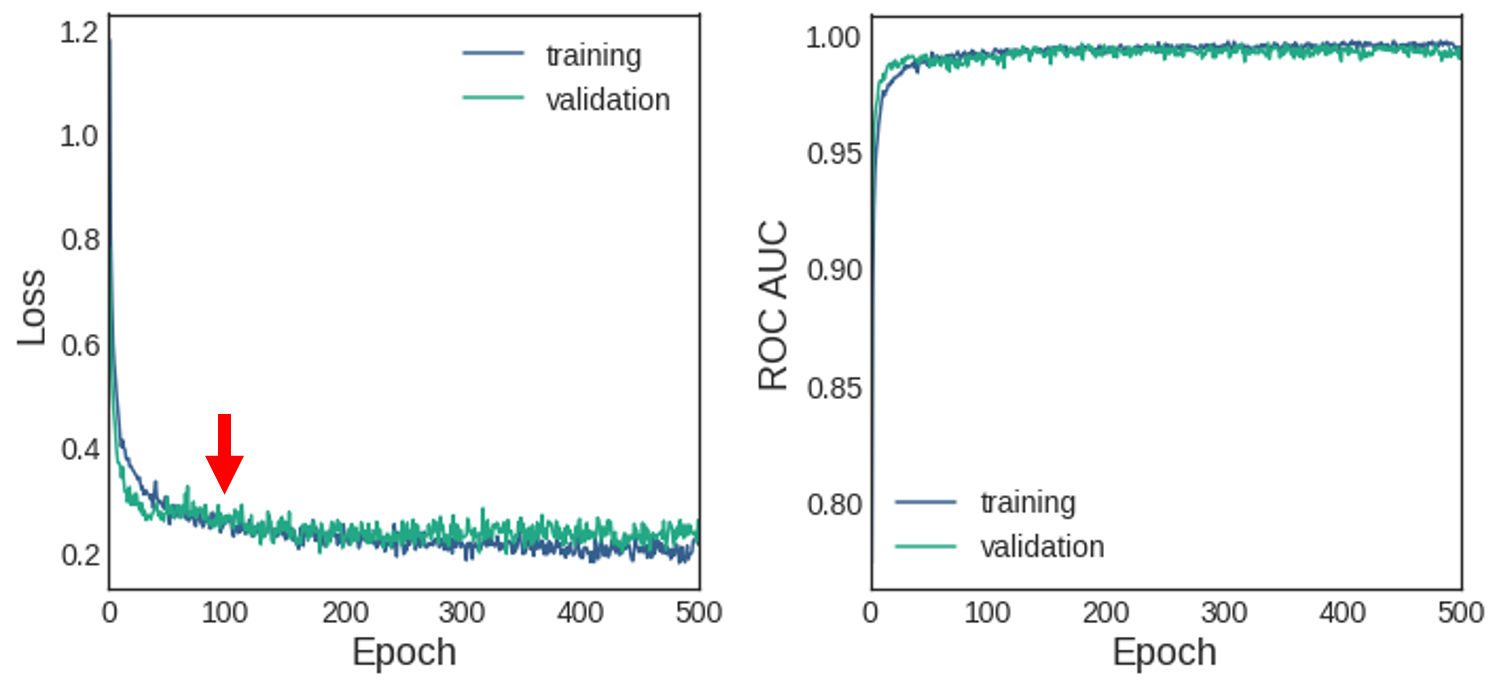
\includegraphics[width=\textwidth]{templates/images/Figure-NN-Training-Loss.png}
\caption[Neural network training loss]{NN training results as a function of epoch count for WDS4. Calculated loss (Left) and AUC (Right) for the training (blue) and validation (green) subsets converge and start to separate near the 100-epoch mark (red arrow). Mini-batch related noise obscures the exact cross-over location.}
\label{fig:nn_loss_plot}
\end{figure}

Tuning was conducted in the same order as listed in Figure \ref{fig:nn_tuning_plots}. Distinct maxima in CV-averaged AUC are observed for each hyperparameter. The selected values for the final WDS4 model include: learning rate of 0.01, $\lambda$ value of $2\times10^{-4}$, batch size of 100, and drop rate of 0.1. Minima in the average loss curves align with the selected hyperparameter values for all except $\lambda$, the regularization parameter on model weights. This matches the expected behavior described in Equation \ref{eq:nn_cost_function}, where $\lambda$ controls the balance between loss and sum of squared weights in the cost function. As Figure \ref{fig:nn_tuning_plots}B shows, the loss term decreases as $\lambda$ approaches zero.

Figure \ref{fig:nn_loss_plot} illustrates the WDS4 training progress as a time series of loss and AUC. The variance in both plots reflects noise introduced by mini-batch training, but convergence takes place quickly. The growing separation between the training and validation loss at greater epoch counts indicates the model is overfitting the training data. The cross-over of the training and validation lines, which corresponds with the tuned value for the epoch hyperparameter, occurs somewhere close to 100 epochs for WDS4.

\subsubsection{Optimized Model Results}

The NN model was re-trained for each of the three data sets using the hyperparameter values listed in Table \ref{tab:nn_tuning}. Data sparsity is problematic for the WDS model; even after careful tuning, the out-of-sample accuracy doesn't exceed 75\%, and test set AUC is just $\approx 86\%$. Data augmentation in WDS4 and WDS8 proves quite beneficial by comparison. Models trained on both expanded data sets exhibit $\approx95\%$ accuracy and AUC values $>99\%$ (Table \ref{tab:nn_tuning}).
 
%\begin{wrapfigure}{R}{0.50\linewidth}
\begin{figure}[htp]
\centering
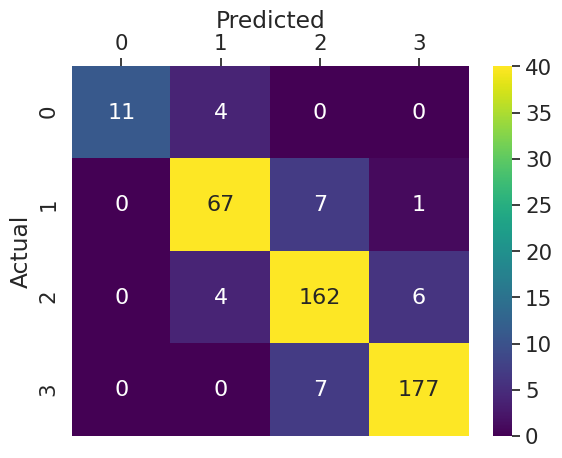
\includegraphics[width=.5\textwidth]{templates/images/Figure-NN-ConfusionMatrix_WDS4.png}
\singlespacing
\caption[Neural network confusion matrix]{Confusion matrix for the tuned NN model trained on WDS4.}
\label{fig:nn_confusion_matrix}
%\end{wrapfigure}
\end{figure}

Figure \ref{fig:nn_confusion_matrix} depicts the confusion matrix constructed from WDS4 model results. Similar to XGB model performance, nearly all of the noted misclassifications are off by only a single class assignment, the largest (19 total) being between medium-grade (class 2) and high-grade (class 3) geothermal gradient. Overall, these are very strong results for a predictive classifier.

Figure \ref{fig:nn_auc} shows the macro average, micro average, and individual class NN ROC curves. All individual class AUC values are at or above 0.99, as was the case for the XGB model. This is close to an ideal ROC plot for a classifier.

\begin{figure}[htp]
\centering
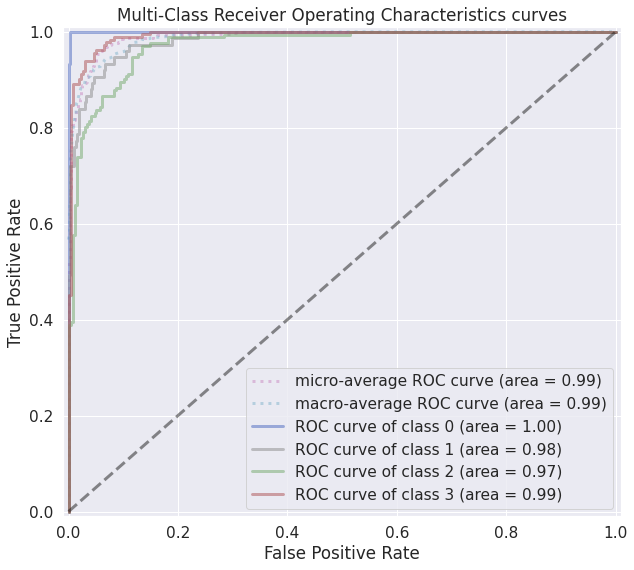
\includegraphics[width=0.7\textwidth]{templates/images/Figure-NN-AUC.png}
\caption[Neural network ROC curves]{ROC curves for tuned NN model trained on WDS4.}
\label{fig:nn_auc}
\end{figure}

\begin{figure}[!htp]
\centering
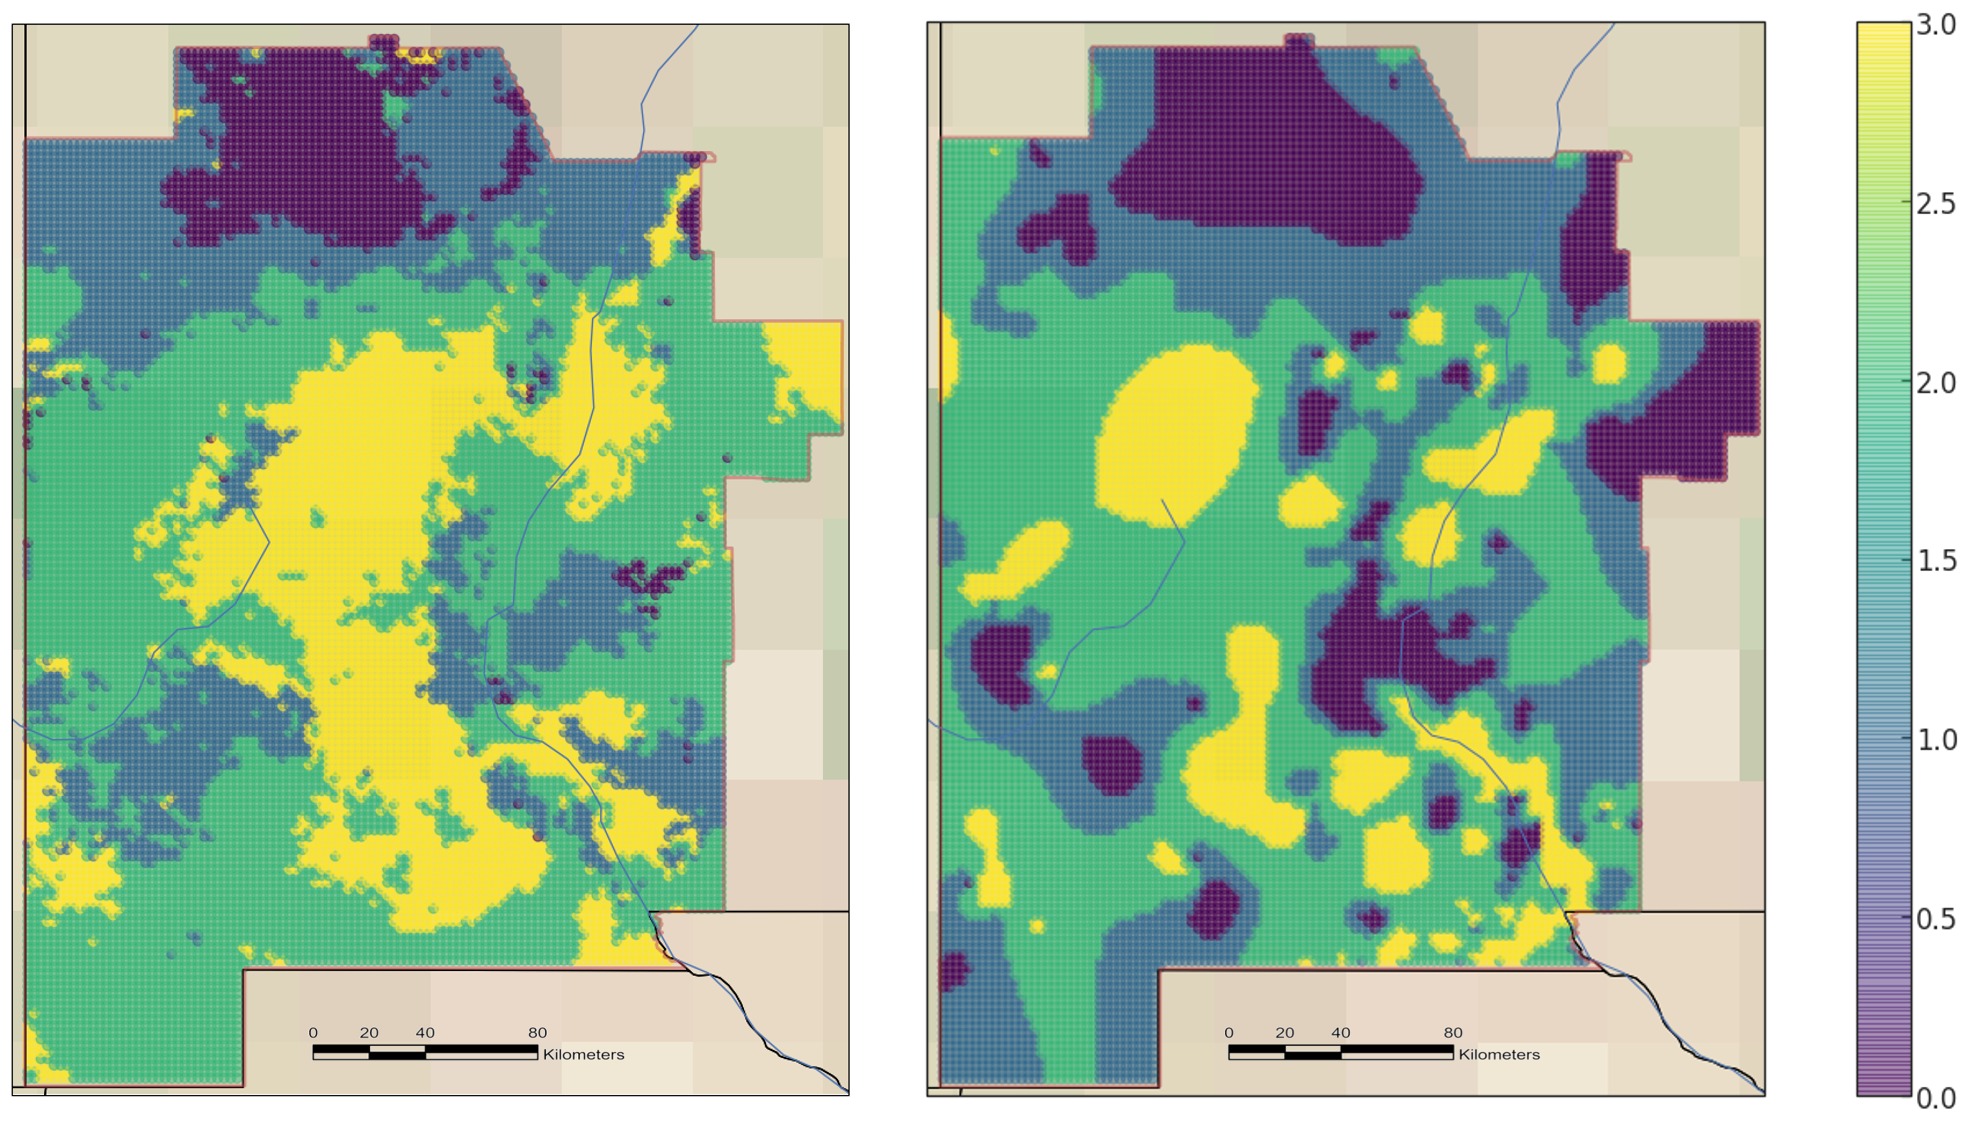
\includegraphics[width=\textwidth]{templates/images/Figure-NN-FinalMap_Joint.png}
\caption[Neural network final map]{Left: Map predictions of geothermal gradient from the tuned NN model trained on WDS4. Right: geothermal gradient data layer from southwestern NM PFA study \protect\citep{bielicki_hydrogeolgic_2015}.}
\label{fig:nn_final_map}
\end{figure}

The FDS was passed through the NN model to generate predictions for the southwestern NM study area as shown in Figure \ref{fig:nn_final_map}. Class 3 high-grade geothermal gradient regions to the southeast in the \citet{bielicki_hydrogeolgic_2015} PFA layer are well-captured by the NN model. The class 3 swath though the center of the AOI describes a broader, more continuous region of geothermal potential than suggested by the PFA map. Additional high-gradient patches unique to the NN map appear along the study area edges – in the southwest corner, eastern AOI extension, and to the northeast paralleling the Rio Grande river. The low-gradient zone to the north matches between the two maps, but most other class 0 areas in the \citeauthor{bielicki_hydrogeolgic_2015} map are not observed in the NN map. Interestingly, there appears to be greater overall similarity between the NN map in Figure \ref{fig:nn_final_map} and the XGB map in Figure \ref{fig:xgb_final_map} than with the PFA map.

%\newpage 
%\subsection{Uncertainty Analysis}
\section{Uncertainty Analysis}

%\begin{wrapfigure}{R}{0.45\textwidth}
%\centering
%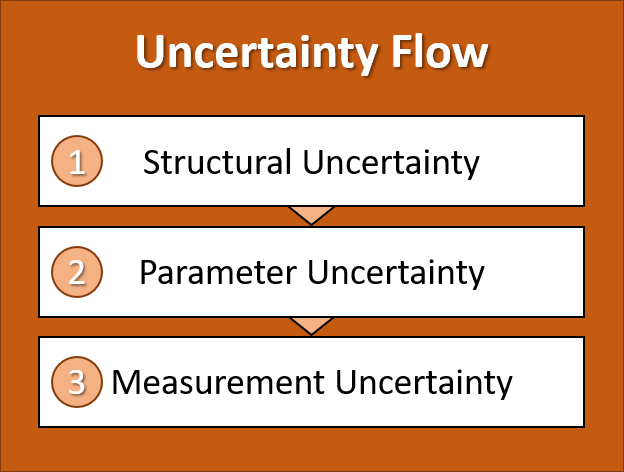
\includegraphics[width=.4\textwidth]{templates/images/Flow-Uncertainty.png}
%\singlespacing
%\caption[Uncertainty analysis workflow]{Workflow for analyzing uncertainties in model results for geothermal gradient prediction across the southwestern NM study area.}
%\label{fig:uncertainty_flow}
%\end{wrapfigure}

%The results obtained from the four supervised machine learning methods discussed so far all match the well data sets with at least an accuracy of 70\%, and in some cases in excess of 95\%. From a statistical perspective, each model accomplishes the task of learning from existing data reasonably well. And they all use those learnings to predict geothermal gradient classifications across the entire AOI. But presenting these results to an explorationist will invariably elicit two important questions: 1) Which of these model results is the right one? and 2) What actions should I take based on these models? 

%George Box's famous statement, “Essentially, all models are wrong, but some are useful” \citep{box_empirical_1987} effectively answers the first question. But knowing that none of the prediction maps is individually correct falls short of providing impactful and actionable information for geothermal exploration decision-makers. Value lies in describing the sources of uncertainty and where those uncertainties manifest in a spatial prediction of geothermal gradient or other modeled attributes. To this end, the following analysis considers uncertainties from the three sources described in Section \ref{ch2:uncertainty} and illustrated in Figure \ref{fig:uncertainty_flow}: model type (structural), model calibration (parameter), and model input (measurement).

%\subsubsection{Classification Uncertainty Measures}

%Unlike standard regression problems that result in continuous variable predictions, classifiers are inherently limited to selecting among $n$ discrete classes. Statistical measures of variability in model results cannot be calculated by methods like standard deviation. For geospatial classifications, the most basic comparison between two maps is visual; plotting two maps side-by-side as in Figure \ref{fig:nn_final_map} can effectively communicate qualitative differences. Quantifying the uncertainty of categorical predictions based on multiple realizations defines a more difficult problem, with a variety of different statistical approaches to consider. Among these are performance measures based on the class assignments, including the percent correctly classified (accuracy), confusion matrix, ROC AUC, Kappa \citep{cohen_coefficient_1960}, and weighted Tau \citep{ma_tau_1995}. Other methods consider the probabilities that precede the final classification choice, including Brier score \citep{brier_verification_1950} and Shannon entropy \citep{shannon_mathematical_1948}. Rather than perform an exhaustive search through different metrics, this thesis follows the recommendation of \citep{beaudette_accuracy_2020} in characterizing classification uncertainty using entropy. Although the classic entropy calculation does not account for class similarity, it shows good discrimination ability for model results with low, medium, and high stand-out probability for the majority class \citep{beaudette_accuracy_2020}. Entropy can be calculated as shown in Equation \ref{eq:entropy} and normalized to a range of $(0, 1]$ as described here:

%\begin{equation}
%\label{eq:norm_entropy}
%    H = -\frac{1}{\log_2{(n)}}\sum_{i=1}^{n}{p_i \cdot \log_2{(p_i)}} = -\sum_{i=1}^{n}{p_i \cdot \log_n{(p_i)}}
%\end{equation}

%where $p_i$ represents the probability assigned to class label $i$. Entropy maps can be defined using the output probabilities of a single classification model or the results in an ensemble of predictions by first averaging across class probabilities for each map location.


\subsection{Structural Uncertainty}
%\subsubsection{Structural Uncertainty}\label{ch5:model_uncertainty}
%The specific choice of classification algorithm implicitly applies constraints on the solution space for the problem. For example, logistic regression solutions assume there is a linear relationship between predictor variables and the log-odds of the response variable. And decision trees use hard thresholds that can create step-like model behavior. 

Figure \ref{fig:combined_maps} shows the four machine learning model results for the southwestern NM AOI. Not only do the models differ in how individual areas are classified, but the overall character of the predictions suggests each model has a signature predictive style.

\begin{figure}[!htp]
\centering
\includegraphics[width=\textwidth]{templates/images/Figure-All_Models.png}
\caption[Combined machine learning results]{Machine learning results for WDS4 using A. logistic regression, B. a decision tree, C. XGBoost, and D. an artificial neural network. Results match those already shown in Figures \ref{fig:logreg_final_map}, \ref{fig:dtree_final_map}, \ref{fig:xgb_final_map}, and \ref{fig:nn_final_map}.}
\label{fig:combined_maps}
\end{figure}

%In order to examine the uncertainty introduced by structural aspects of the chosen machine learning models, the predicted class probabilities for each model output were averaged together to create an ensemble prediction of geothermal gradient classes.

Figure \ref{fig:avg_final_map}A depicts the result when each map location is assigned to the dominant average class probability. Aspects of all four models in Figure \ref{fig:combined_maps} can be identified in this result, but the overall effect is a simpler model with a more spatially-conservative high-grade class 3 predictions. Also missing are many of the spurious high-gradient patches along the AOI boundaries and within the eastern and southern AOI extensions. The \citeauthor{bielicki_hydrogeolgic_2015} map (Figure \ref{fig:avg_final_map}B) depicts much more structure in geothermal gradient predictions, with a pock-marked appearance due to classification bulls-eye patterns.

\begin{figure}[!htp]
\centering
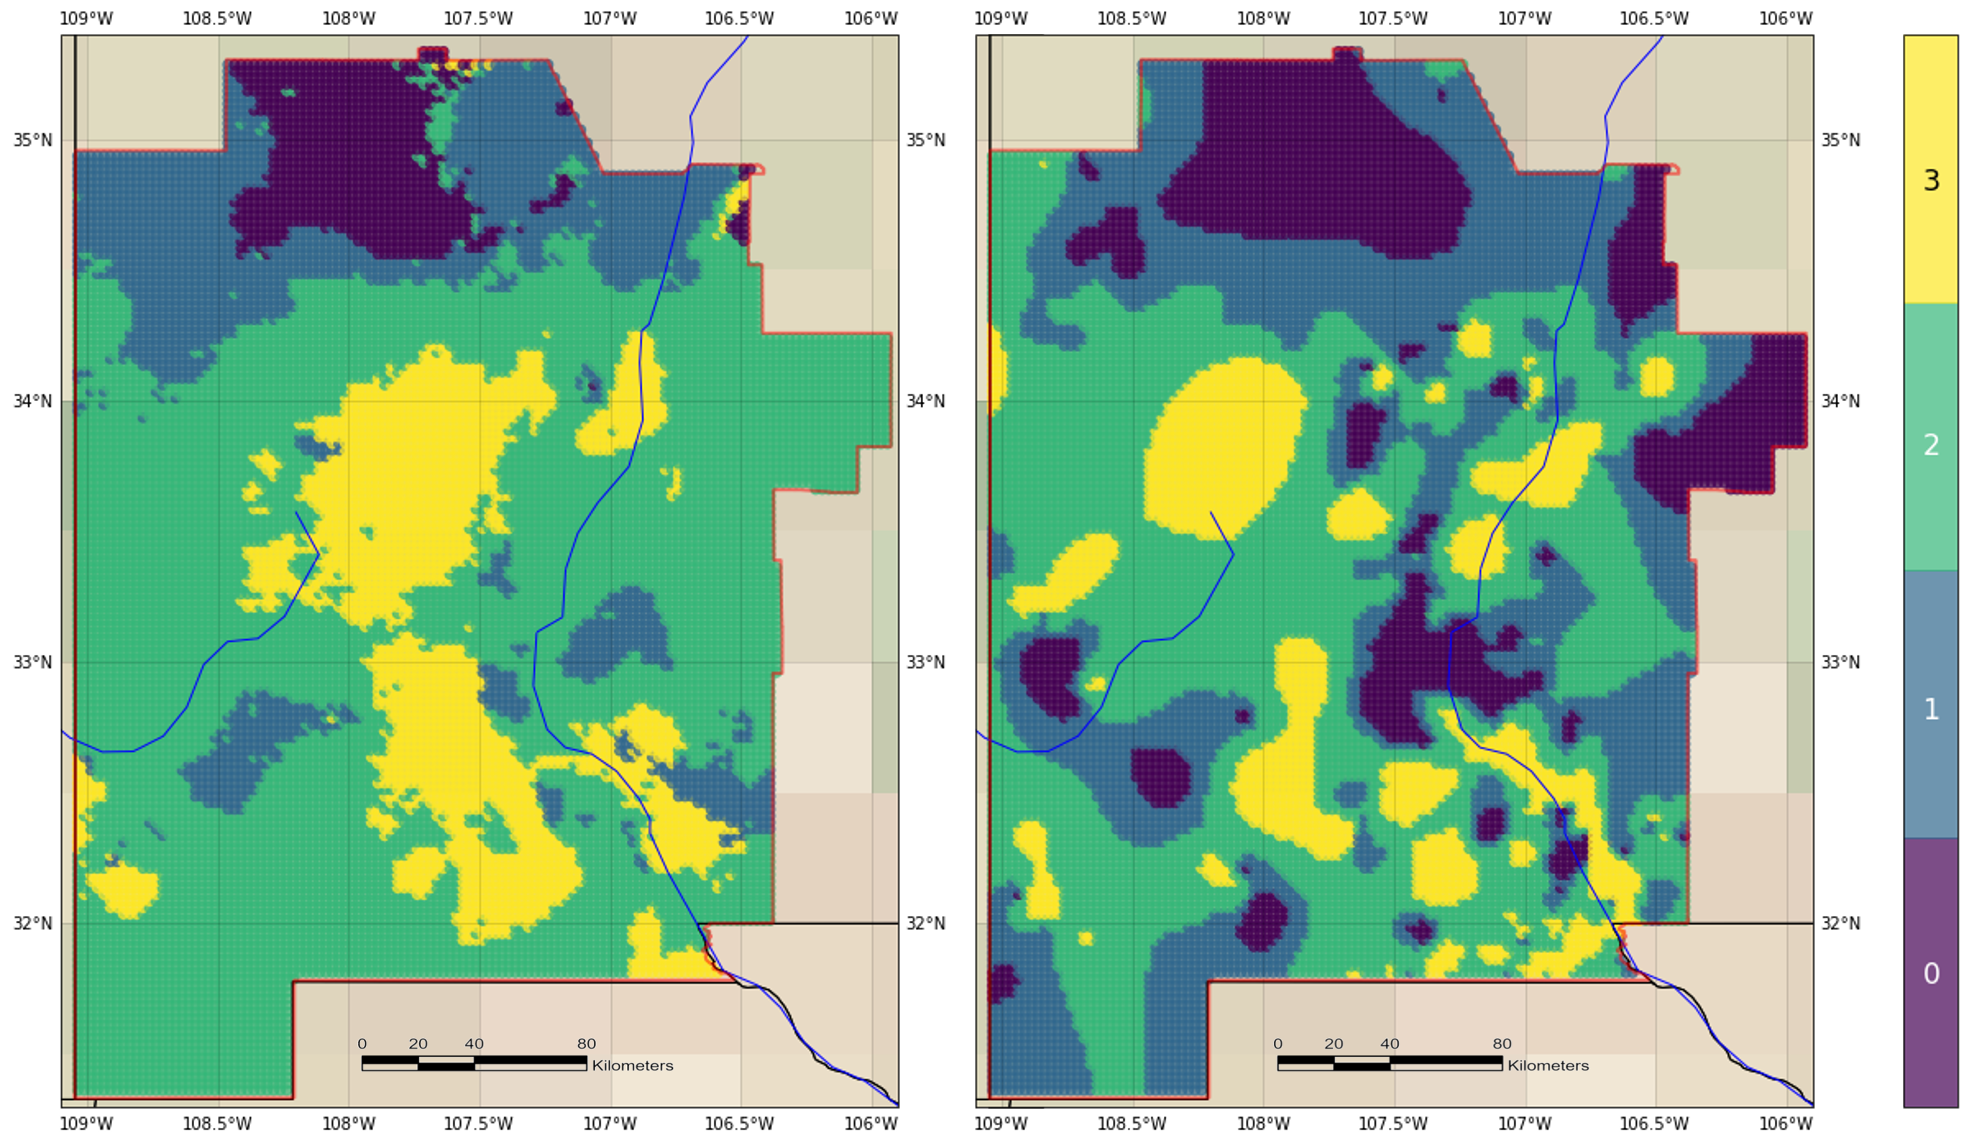
\includegraphics[width=\textwidth]{templates/images/Figure-Average_Gradient_Map_Joint.png}
\caption[Probability-averaged prediction map]{Left: Geothermal gradient classification map based on the average class probabilities from the predictive models shown in Figure \ref{fig:combined_maps}. Results are based on WDS4. Right: geothermal gradient data layer from southwestern NM PFA study \protect\citep{bielicki_hydrogeolgic_2015}.}
\label{fig:avg_final_map}
\end{figure}

%Shannon entropy is calculated on this same averaged model data set using the class probabilities, not just the dominant class. 
The result is shown in Figure \ref{fig:structural_entropy_map}A. Normalized entropy values vary from 0 to 1, with high entropy defining locations where there is no clear differentiation between gradient class label probabilities. Regions colored red thus identify locations that are difficult for any model to classify based on inconclusive feature inputs, or alternatively, locations where the predicted class probabilities from the different models varied enough that, upon averaging, they converged to similar values and could not be disentangled.

Figure \ref{fig:structural_entropy_map}B illustrates an alternative way of presenting these results. Regions of high entropy (over 0.7) are masked in dark gray because of the uncertainty in their classifications. All other points have a level of transparency that scales with entropy. Low uncertainties/entropy values are scarce, focused primarily in the southwest and in small patches to the central west and central east areas. High uncertainties track the borders between geothermal classifications to the north and southeast. In the Colorado Plateau region, they form a ring around an area of low-grade geothermal gradient (class 0). This highlights model inconsistencies on exactly where the class 0-class 1 boundary should appear based on trends in the input feature data.

\begin{figure}[!htp]
\centering
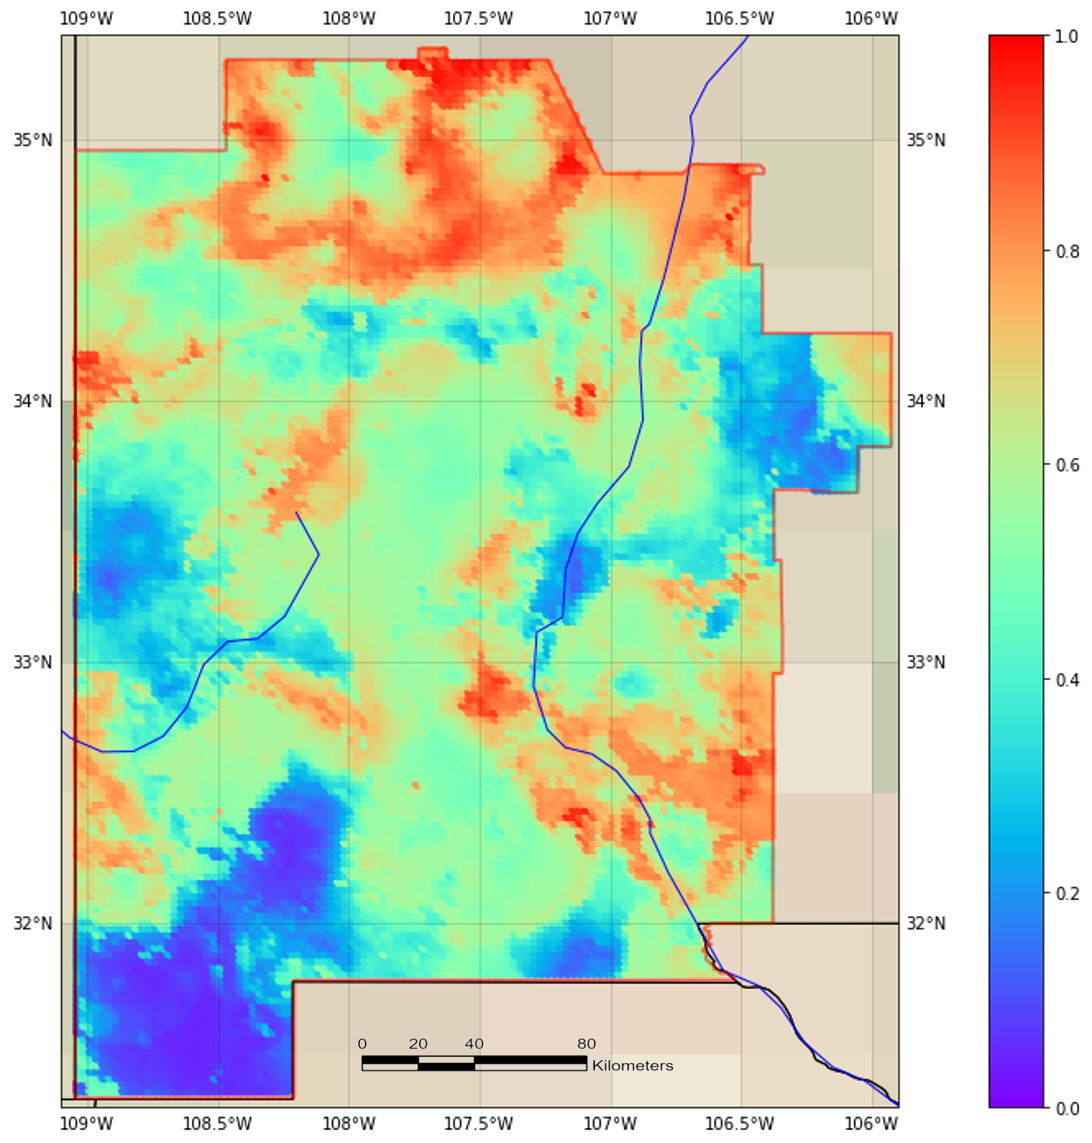
\includegraphics[width=.8\textwidth]{templates/images/Figure-Structural_Entropy_Map.png}
\caption[Structural uncertainty map]{Structural uncertainty from choice of models, measured using Shannon entropy. Values are normalized to range from 0 for low entropy, low uncertainty (blue) to 1 for high entropy, high uncertainty (red).}
\label{fig:structural_entropy_map}
\end{figure}

\begin{figure}[!htp]
\centering
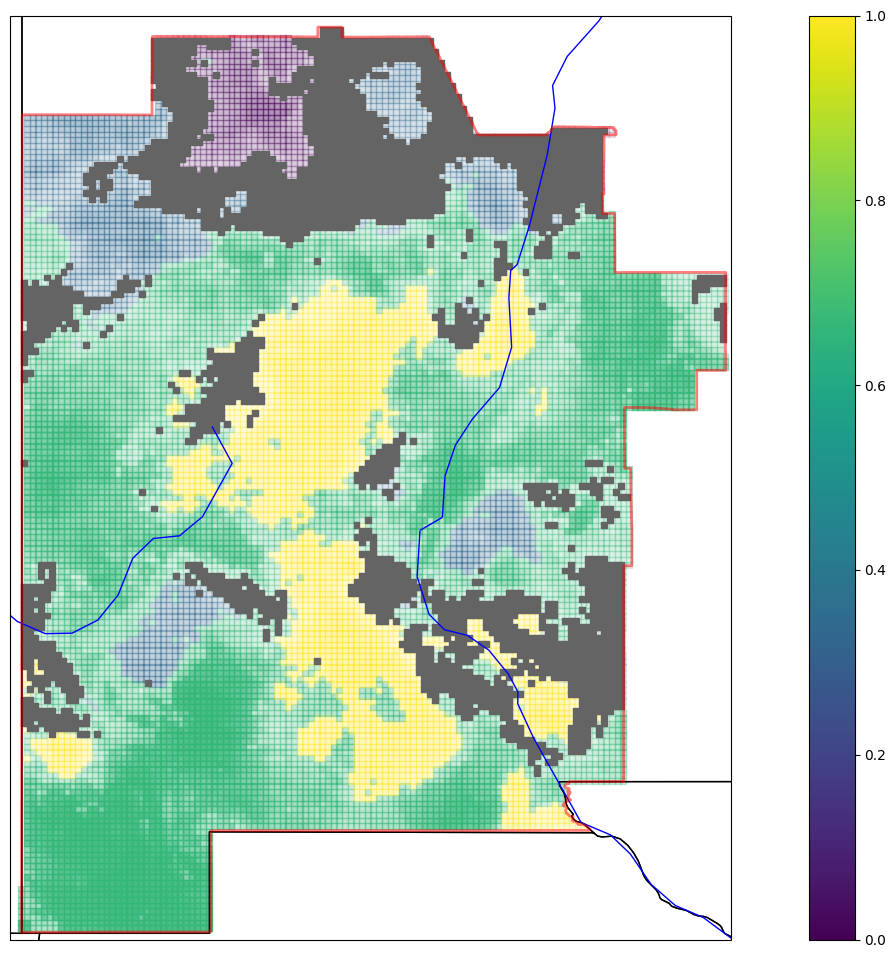
\includegraphics[width=.8\textwidth]{templates/images/Figure-Masked_Average_Gradient_Map.png}
\caption[Structural uncertainty mask on prediction map]{Probability-averaged prediction map with uncertainty masking. Normalized entropy values (>0.7) are grayed out, all others determine transparency of the colored scatter plot. Transparency increases from none at entropy values close to 0 to full for entropy values close to 1. The background topographic raster has been removed to better visualize the transparency effect.}
\label{fig:avg_gradient_masked_map}
\end{figure}

\subsection{Parameter Uncertainty} \label{ch5:param_uncertainty}
%\subsubsection{Parameter Uncertainty} \label{ch5:param_uncertainty}

%The fitting procedure for machine learning models like logistic regression and neural networks involves minimizing a cost function as updates are iteratively made to model parameters, e.g., feature weights. However, the final model solutions typically present these parameters as deterministic values with no uncertainty. The complexity of neural networks, and the potential for different parameterizations as randomness in techniques like dropout and mini-batching influence the training process, suggest such representations under-characterize the model space. By defining the range of uncertainty on model parameters, it is possible to generate many solutions from the same model that define an ensemble of valid predictions. Uncertainty estimates derived from this ensemble can introduce a measure of confidence in a model’s output, allowing the model to directly explain what it knows and, more importantly, what it doesn’t know in the solutions it produces.

%The Google DeepMind team introduced a method called “Bayes by Backprop” in 2015 where single-value weights are replaced by probability distributions in a neural network architecture \citep{blundell_weight_2015}. Making the simplifying assumption that the weight distributions are Gaussian, each weight parameter in a standard NN layer is replaced by a mean and a standard deviation in a probabilistic layer. A fully-trained \acrlong{bnn} (\acrshort{bnn}) samples from the weight distributions for just-in-time determination of weight values as data is fed through to produce a prediction. Therefore, each prediction of the BNN varies depending on the selected weights, and running the network many times on the same data set will produce a set of different results. An analysis of the variation in this solution ensemble can characterize how parameter uncertainty impacts BNN classification performance.

%At a fundamental level, BNNs operate using Bayes theorem for training the network \citep{webster_probabilistic_2021}:

%\begin{equation}
%    \label{eq:bayesrule}
%    P({\bf w} \vert D) = \frac{P(D \vert {\bf w}) \cdot P({\bf w})}{P(D)}
%\end{equation}

%Where ${\bf w}$ are the model weights, $D$ is the observed data. $P({\bf w})$ define the \textit{priors}, or the distributions assigned to the weights before seeing $D$. $P(D \vert {\bf w})$ defines the likelihood of $D$ given $w$. $P({\bf w} \vert D)$ are the \textit{posteriors} or the distributions after taking $D$ into account.

%In practice, BNNs use a Variational Bayes method, which approximates $P({\bf w} \vert D)$ with a variational posterior, $q({\bf w} \vert \theta)$. The desired difference between these two functions is zero (perfect approximation), so this defines the basis of a loss function measured using the Kullback-Leibler divergence \citep{webster_probabilistic_2021}:

%\begin{equation}
%    \label{eq:bnn_loss}
%    \begin{aligned}
%    D_{KL}\left(q({\bf w} \vert \theta)\ \vert\vert\ P({\bf w} \vert D)\right) &= \int{q({\bf w} \vert \theta) \log \left({\frac{q({\bf w} \vert \theta)}{P({\bf w} \vert D)}}\right) d{\bf w}} \\
%    &= \log P(D) + D_{KL}\left(q({\bf w} \vert \theta)\ \vert\vert\ P({\bf w})\right) \\ 
%    &\qquad- \mathbf{E}_{q({\bf w} \vert \theta)}\left[\log P(D \vert {\bf w})\right]
%    \end{aligned}
%\end{equation}
%Dropping constant terms and treating this as an objective to minimize \citep{blundell_weight_2015}:
%\begin{equation}
%    \label{eq:bnn_objective}
%    J(\Theta) = D_{KL}\left(q({\bf w} \vert \theta)\ \vert\vert\ P({\bf w})\right) - \mathbf{E}_{q({\bf w} \vert \theta)}\left[\log P(D \vert {\bf w})\right]
%\end{equation}

%This two-term objective describes a trade-off between the complexity as controlled by deviation from the prior ($P({\bf w})$) and the negative log-likelihood term measuring the fit to the data.

The TensorFlow Probability package was used to transform the NN from Section \ref{ch5:ann_model} into a BNN for uncertainty estimation \citep{dillon_tensorflow_2017}.  Given the sparsity of training data available and the multiplier effect that probabilistic layers have on the number of trainable parameters in a BNN, only the second hidden layer was converted to a TensorFlow \textit{DenseVariational} layer (Figures \ref{fig:bnn_text_structure} and \ref{fig:bnn_dot_structure}). Standard normal ($N(0,1)$) distributions were used as priors for the layer nodes. All hyperparameter values tuned for the dataset-specific neural networks (Table \ref{tab:bnn_metrics}) were also applied to the BNNs with one exception: the number of epochs was increased by a factor of 3-4. Figure \ref{fig:bnn_loss} shows the training loss and AUC curves for WDS4, which justify this larger number of epochs for training. Table \ref{tab:bnn_metrics} notes the accuracy and AUC scores for the BNNs calculated from a single predictive run on the respective test data subsets.

\begin{figure}[!htp]
\centering
\begin{minipage}[b][][b]{.35\linewidth}
    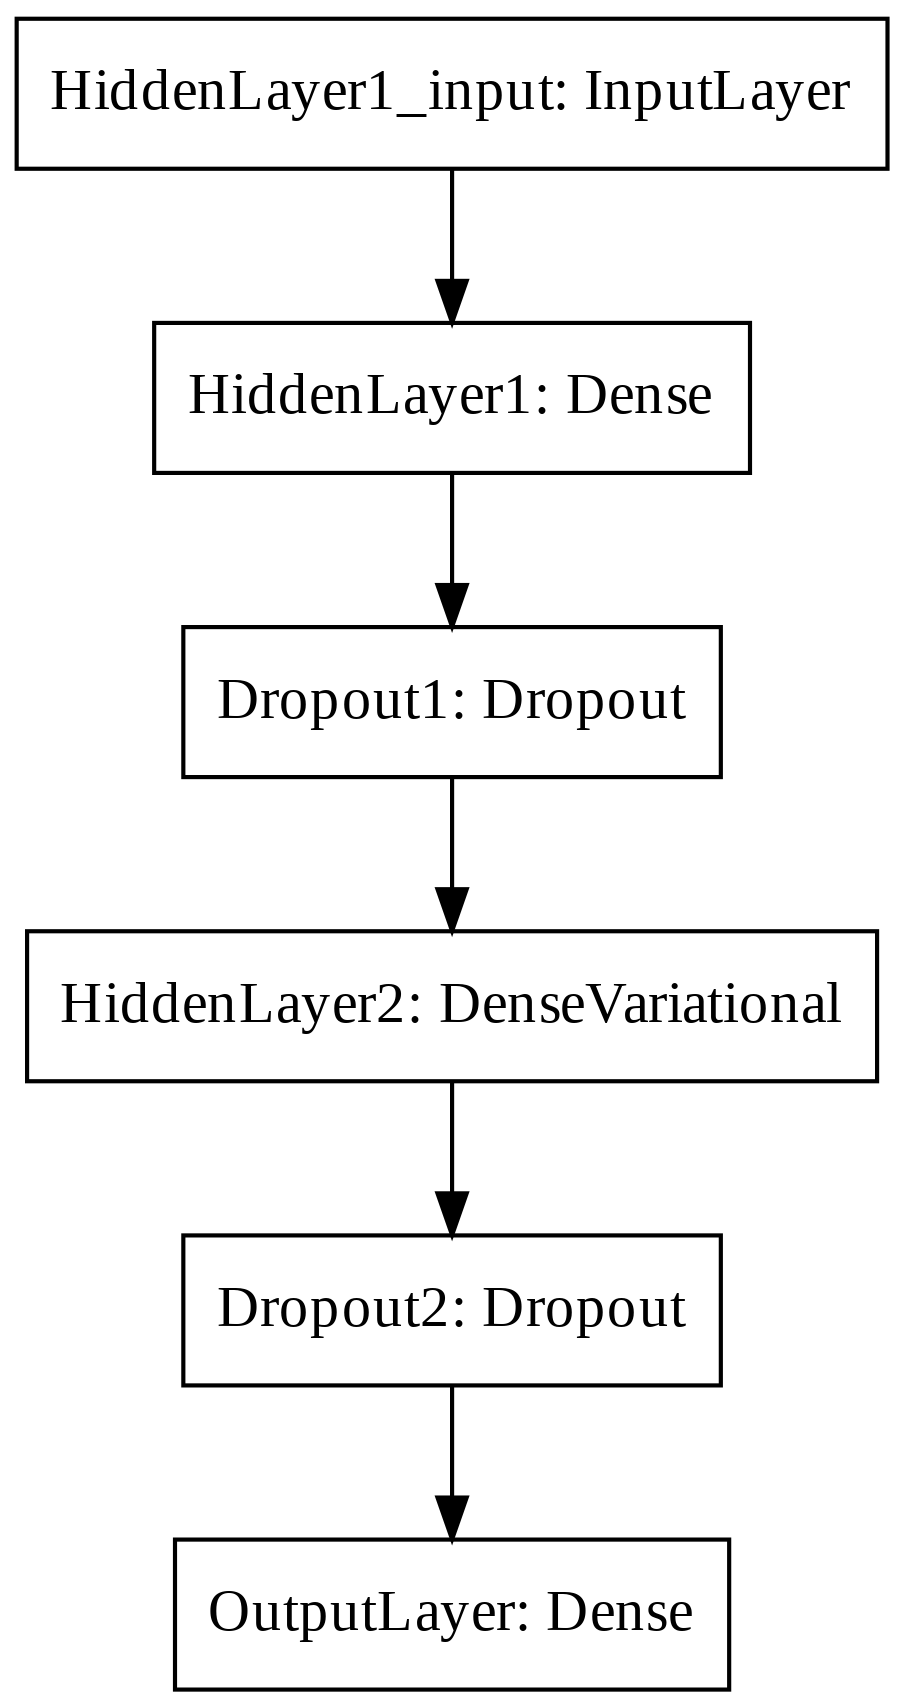
\includegraphics[width=\linewidth]{templates/images/Figure-TF_BNN_Structure.png}
    \caption[Bayesian neural network structural flow]{Structural flow chart for the Bayesian neural network.}
    \label{fig:bnn_text_structure}
\end{minipage}
\hfill
\begin{minipage}[b][][b]{.61\linewidth}
    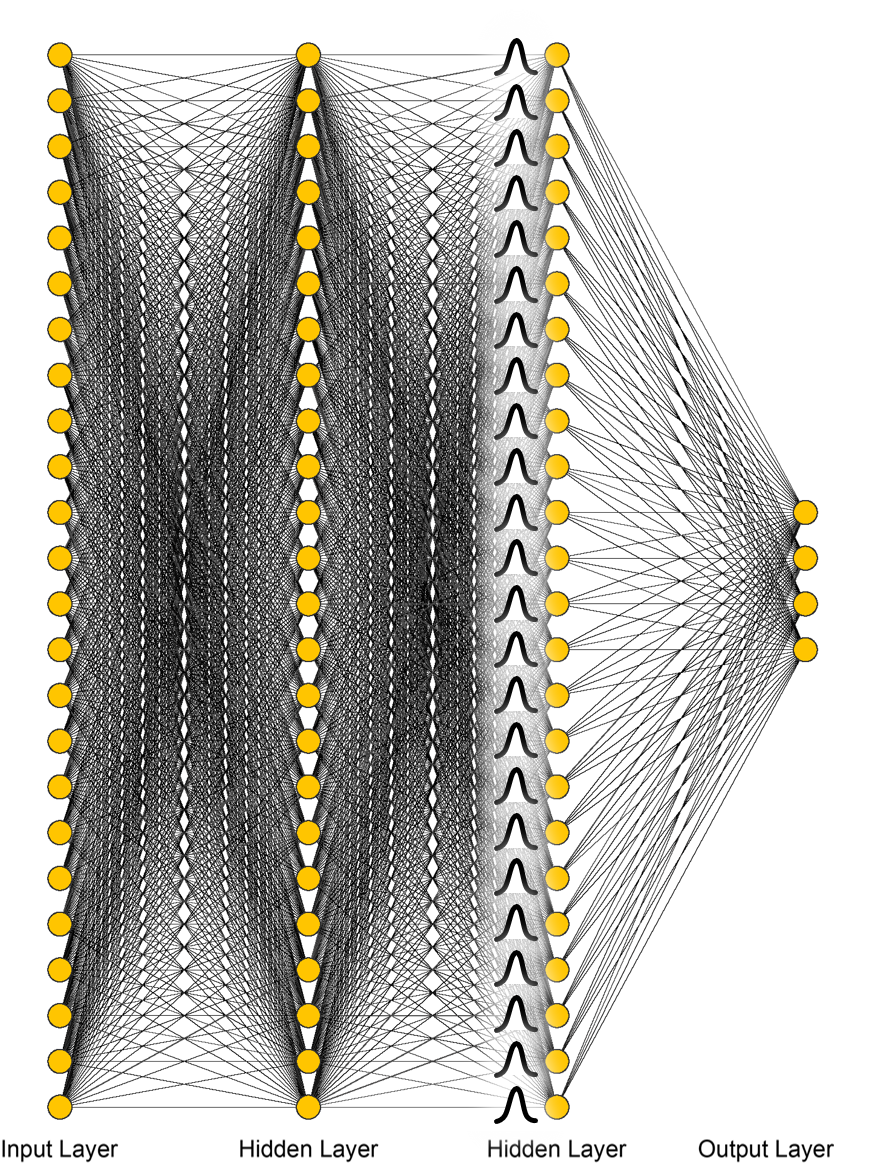
\includegraphics[width=\linewidth]{templates/images/Figure-BNN.png}
    \caption[Bayesian neural network structural schematic]{Schematic diagram of the Bayesian neural network. Not shown are the dropout operations after each hidden layer.}
    \label{fig:bnn_dot_structure}
\end{minipage}
\end{figure}

\begin{table}[htp]
\centering
\begin{tabular}{l|c|c|c|}
\cline{2-4}
                                      & WDS   & WDS4  & WDS8  \\ \hline
\multicolumn{1}{|l|}{learning rate}   & 0.005 & 0.010 & 0.010 \\ \hline
\multicolumn{1}{|l|}{lambda ($\lambda$)} & 1E-04 & 2E-04 & 1E-04 \\ \hline
\multicolumn{1}{|l|}{batch size}      & 50    & 100   & 150   \\ \hline
\multicolumn{1}{|l|}{dropout rate}    & 0.3   & 0.1   & 0.1   \\ \hline
\multicolumn{1}{|l|}{epochs}          & 100   & 300   & 600   \\ \hline
\multicolumn{1}{|l|}{Accuracy$_{train}$} & 0.516 & 0.867 & 0.902 \\ \hline
\multicolumn{1}{|l|}{Accuracy$_{test}$}  & 0.483 & 0.869 & 0.894 \\ \hline
\multicolumn{1}{|l|}{AUC$_{train}$}      & 0.798 & 0.976 & 0.990 \\ \hline
\multicolumn{1}{|l|}{AUC$_{test}$}       & 0.762 & 0.961 & 0.980 \\ \hline
\end{tabular}
\singlespacing
\caption[Bayesian neural network single-run metrics]{BNN hyperparameters used for training and test results for each data set. Accuracy and AUC metrics are split into train (in-sample) and test (out-of-sample) values. Results reflect a single prediction from the BNNs and will vary due to the stochastic nature of the feed-forward BNN operation.}
\label{tab:bnn_metrics}
\end{table}

\begin{figure}[!htp]
\centering
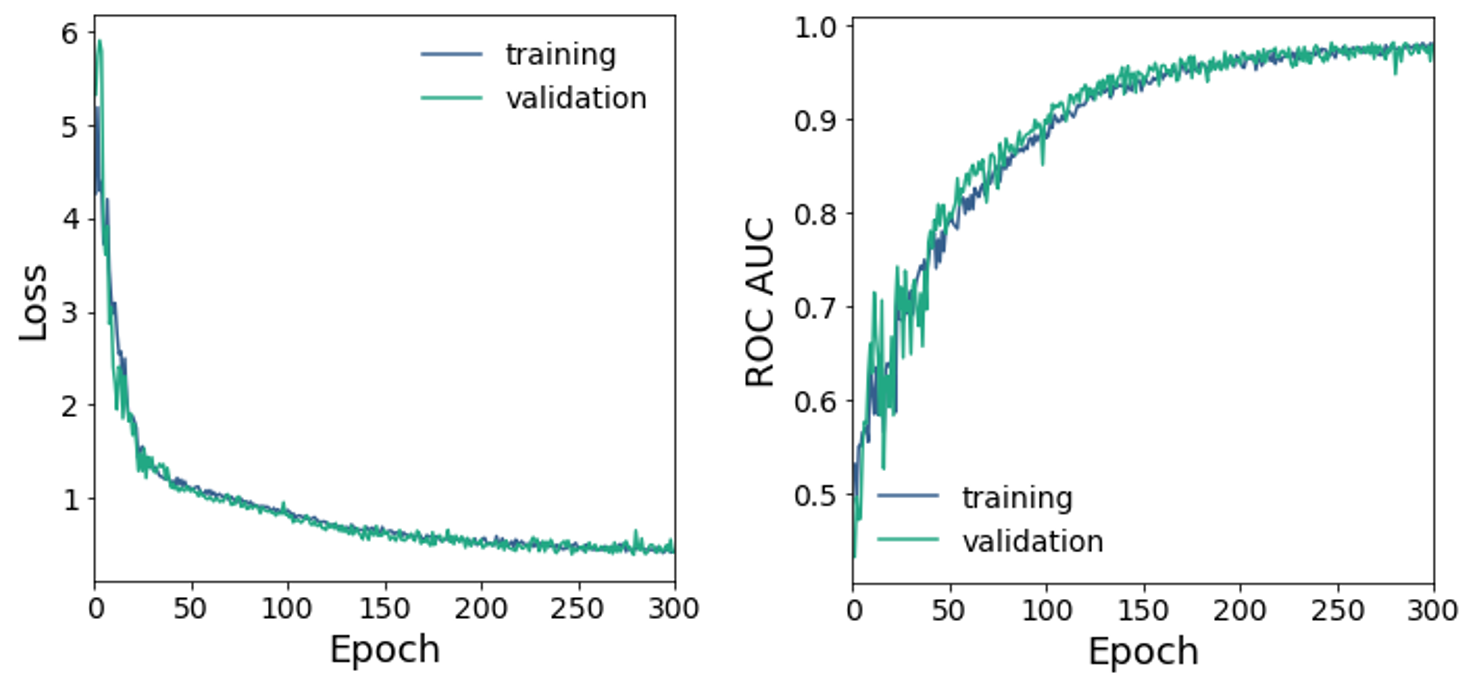
\includegraphics[width=\textwidth]{templates/images/Figure-BNN_Loss_AUC_WDS4.png}
\caption[Bayesian neural network training loss]{BNN training results as a function of epoch count for WDS4. Calculated loss (Left) and AUC (Right) for the training (blue) and validation (green) subsets show training convergence by $\approx 300$ epochs. The stochastic nature of the BNN makes the AUC/epoch curve noisier than for the deterministic NN (Figure \ref{fig:nn_loss_plot})}
\label{fig:bnn_loss}
\end{figure}

Running the BNN multiple times will produce a collection of different results. Figure \ref{fig:bnn_class_pdfs} shows the range of class label probabilities after predicting the classification of 3 well records 100 times using a BNN trained on the WDS4 training subset. Here, the relationship between entropy values and the overlap in class label probabilities is apparent. A low entropy scenario (Figure \ref{fig:bnn_class_pdfs}A) has strong stand-out between the maximum-probability class label and others, while high entropy situations (Figure \ref{fig:bnn_class_pdfs}C) have less certainty on the class label assignment.

\begin{figure}[!htp]
\centering
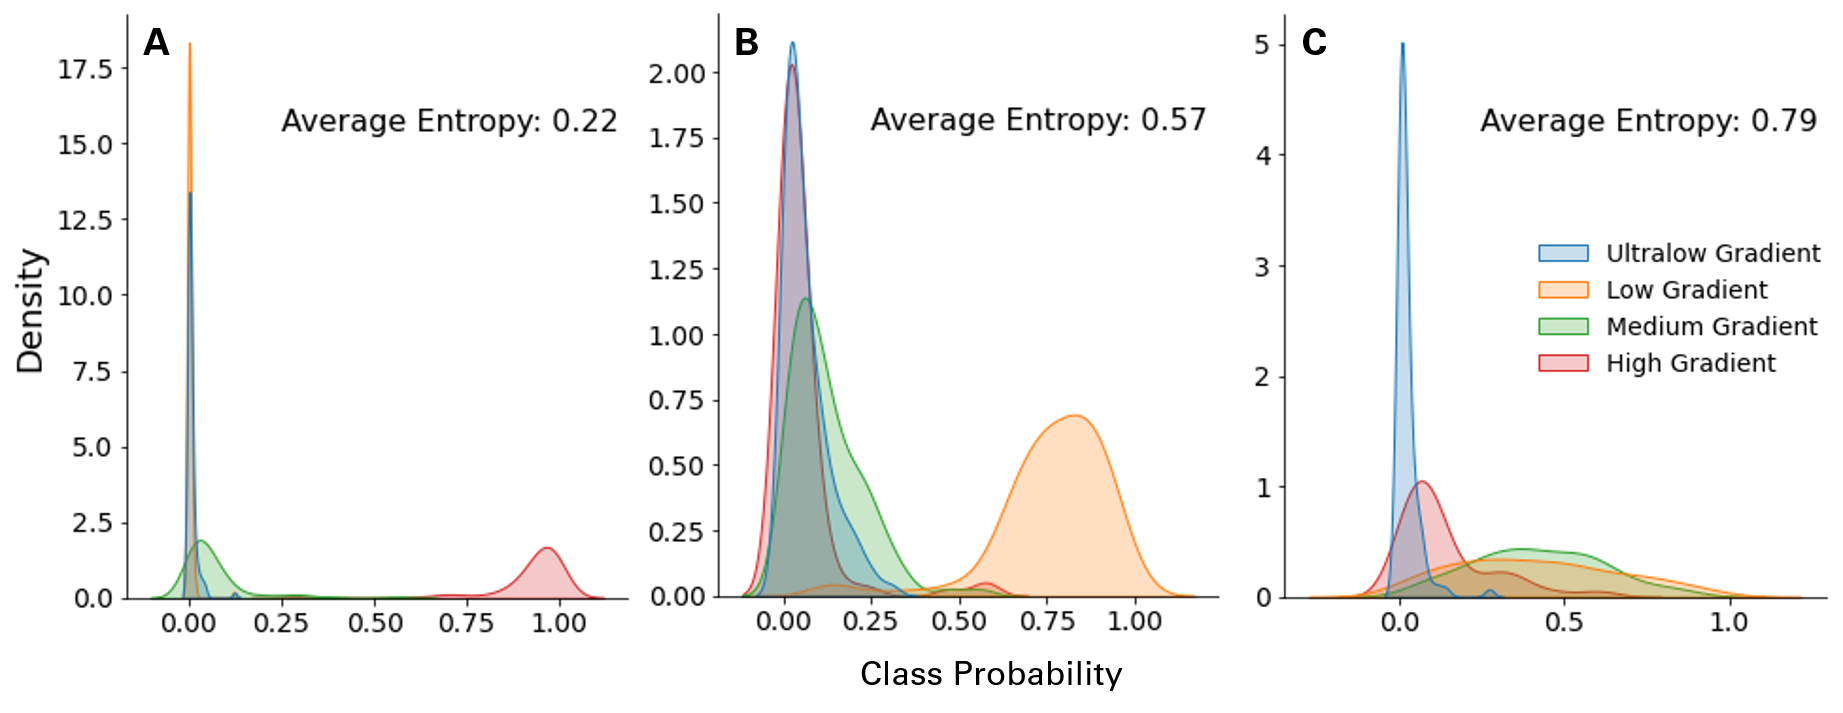
\includegraphics[width=\textwidth]{templates/images/Figure-BNN_100trials_WDS4.png}
\caption[Bayesian neural network class pdfs]{Example class label probability density functions for A. well record 34, B. well record 20, and C. well record 35 from WDS4. Distributions are constructed from 100 passes through the WDS4 BNN. Entropy values scale with label distribution entanglement. The predicted label is the one with the highest mean probability: A. High gradient, B. Low gradient, C Medium gradient.}
\label{fig:bnn_class_pdfs}
\end{figure}

After re-training the BNN on the full WDS4 data set, predictions for the entire AOI were generated 1000 times. Geothermal gradient class probabilities from these realizations were averaged by class for each point location, and the maximum probability class was selected as the predicted label. Entropy values calculated from the ensemble-averaged probabilities are shown in Figure \ref{fig:bnn_entropy_map}. Figure \ref{fig:bnn_masked_pred_map} combines the 1000-run average prediction map with parameter uncertainties using a layer mask and transparency. Concentrated areas of high entropy/uncertainty appear to the southeast in the Rio Grande Rift province, and to the north within the Colorado Plateau and at the RGR-Great Plains province boundary (Figure \ref{fig:bnn_masked_pred_map}). Overall, there appear to be fewer point locations with high entropy in the parameter uncertainty assessment compared to the structural uncertainty analysis for the four model architectures (Figure \ref{fig:avg_gradient_masked_map}).

\begin{figure}[!htp]
\centering
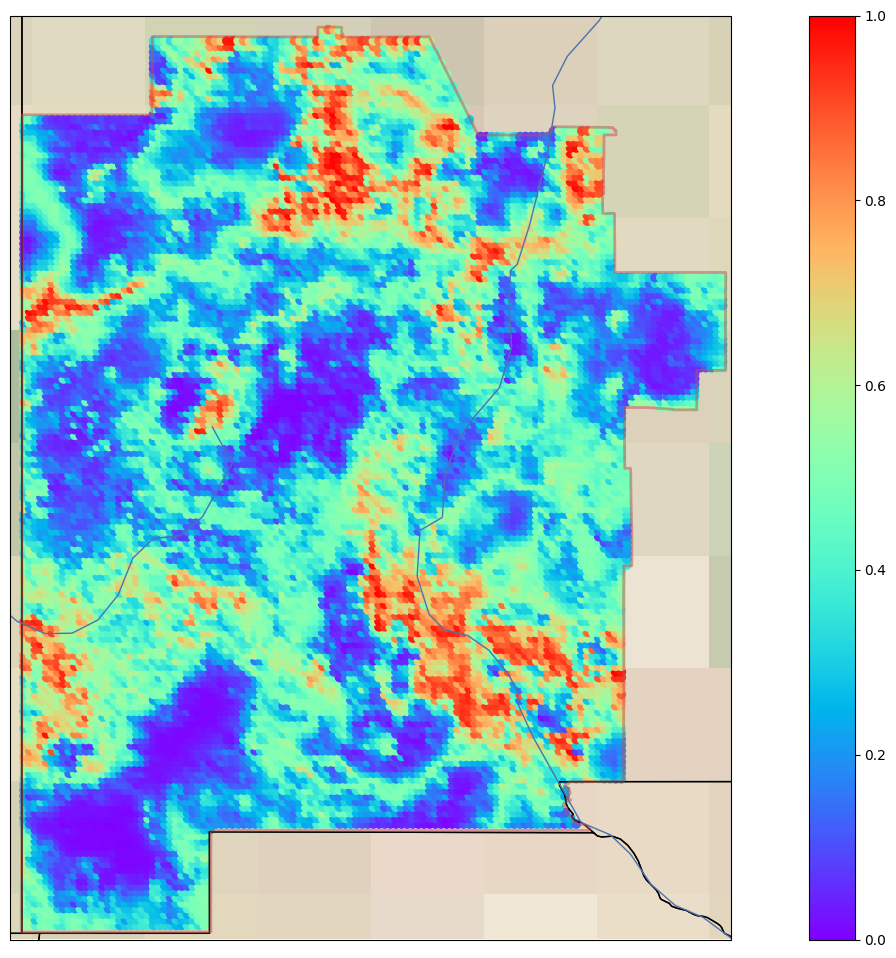
\includegraphics[width=.8\textwidth]{templates/images/Figure-BNN_Entropy_Map.png}
\caption[BNN parameter uncertainty map]
{BNN parameter uncertainty determined from class probability averages after 1000 runs of the WDS4 predictive model. Uncertainty is measured with normalized Shannon entropy values ranging from 0 for low entropy, low uncertainty (blue) to 1 for high entropy, high uncertainty (red).}
\label{fig:bnn_entropy_map}
\end{figure}

\begin{figure}[!htp]
\centering
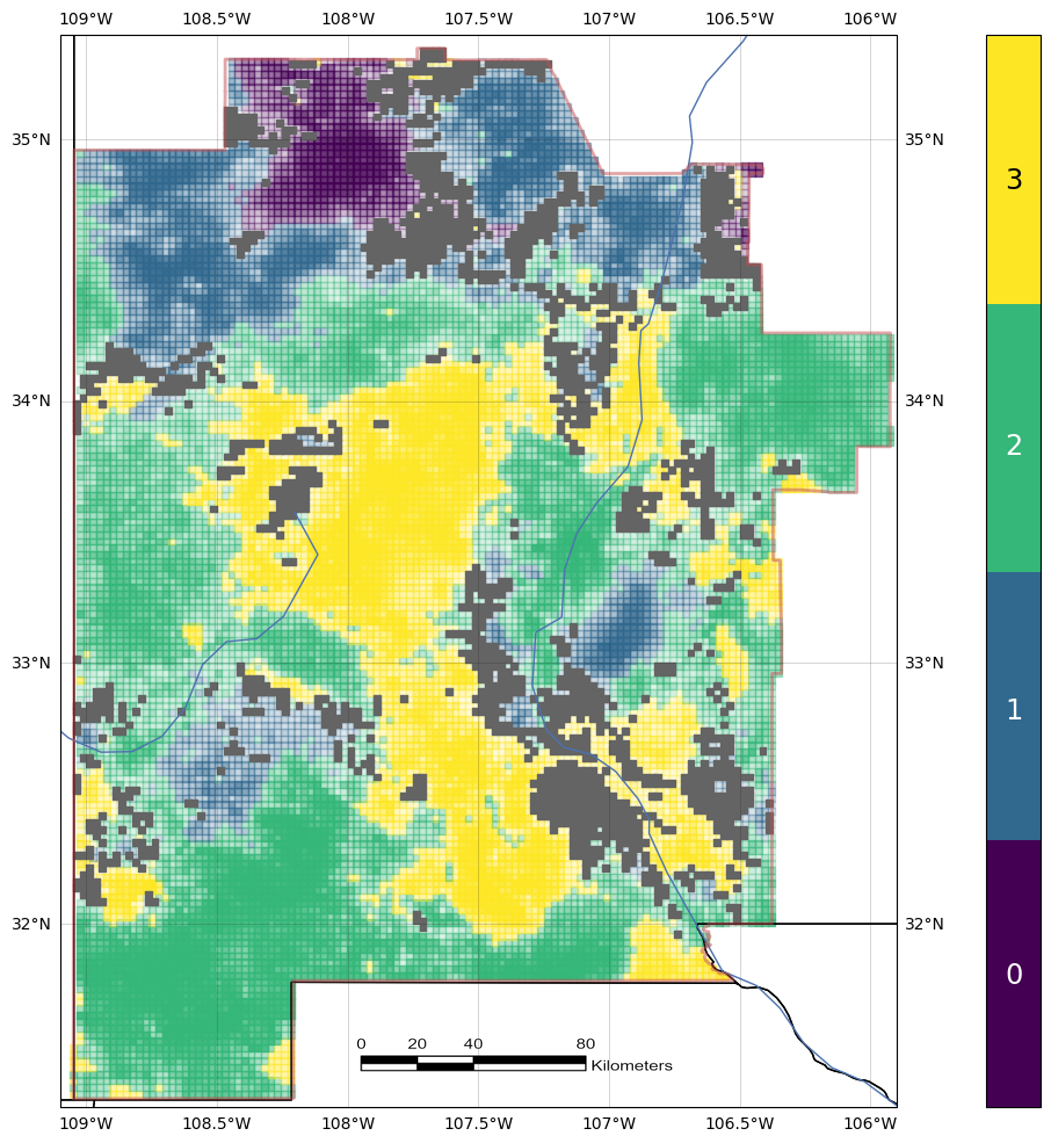
\includegraphics[width=.8\textwidth]{templates/images/Figure-BNN_All_Gradient_Map_Masked_whitebackground.png}
\caption[Parameter uncertainty mask on BNN prediction map]
{Probability-averaged WDS4 BNN prediction map with uncertainty masking. Normalized entropy values (>0.7) are grayed out, all others determine transparency of the colored scatter plot. Transparency increases from none at entropy values close to 0 to full for entropy values close to 1. The background topographic raster has been removed to better visualize the transparency effect.}
\label{fig:bnn_masked_pred_map}
\end{figure}

\subsection{Measurement Uncertainty}\label{ch5:measure_uncertainty}
%\subsubsection{Measurement Uncertainty}\label{ch5:measure_uncertainty}

%Data modeling and analytics generally begin with the collection, engineering, and conditioning of features of interest. Building the perfect dataframe for machine learning may be the first priority, but capturing standard error estimates for its constituent features is fundamental to understanding how much uncertainty they bring to the prediction problem.

In this analysis, the sources of data, types of data, and options for error estimation vary greatly. Several features were acquired as pre-gridded raster files without error assessments or access to the original source data (Table \ref{tab:features}), e.g., air temperature, precipitation, strain rate, and layers from the \citeauthor{bielicki_hydrogeolgic_2015} OpenEI submission \citep{kelley_geothermal_2015}. Table \ref{tab:feature_std_error} shows the top ten features identified by Shapley analysis for the XGBoost model in Section \ref{ch5:xgb_feature_selection}. Among those variables, \acrlong{sigt} (\acrshort{sigt}), Heat Flow, and Boron Concentration have readily-available standard error estimates either from the original source or data preparation process. Crustal Thickness standard error is both unknown and difficult to ascertain; the feature grid comes from contours fit to 2D seismic models \citep{keller_comparative_1991}, which are unavailable for further analysis and review. The remaining top ten features consist of point or line data converted to density layers using KDE. Standard errors could be estimated for these features by performing bootstrap or jackknife resampling, applying KDE on the derivative data sets, and calculating standard errors from that sample population \multicitep{james_introduction_2013, p.\ 187-190;mcintosh_jackknife_2016}.

\begin{table}[htp]
\centering
\resizebox{\textwidth}{!}{
\begin{tabular}{|c|c|c|p{7cm}|}
\hline
\textbf{Name}                     & \textbf{Type}         & \textbf{Std Err Estimation} & \multicolumn{1}{c|}{\textbf{Comments}}             \\ \hline
Si-Geotherm. Temperature & Overlapping points & Kriging & Standard error estimates directly from kriging. \\ \hline
Heat Flow & Non-overlapping points & Directly provided & Standard error estimates provided for each grid point. \\ \hline
Crustal Thickness & Lines & Unknown & Contours based on 2D seismic lines. Uncertainty in interpretation   (e.g., velocity model) unavailable. \\ \hline
Volcanic Dike Density & Lines & Resampling & Jackknife/bootstrap resample and generate density estimates. \\ \hline
Spring Density & Non-overlapping points & Resampling & Jackknife/bootstrap resample and generate density estimates. \\ \hline
Earthquake Density & Overlapping Points & Resampling & Jackknife/bootstrap resample and generate density estimates. \\ \hline
Volcanic Vent Density & Non-overlapping points & Resampling & Jackknife/bootstrap resample and generate density estimates. \\ \hline
Boron Concentration & Overlapping points & Kriging & Standard error estimates directly from kriging. \\ \hline
Quaternary Fault Density & Lines & Resampling & Jackknife/bootstrap resample and generate density estimates. \\ \hline
Drainage Density & Lines & Resampling & If extracted from DEM, relates to DEM slope error. However, can probably use jackknife/bootstrap method. \\ \hline
\end{tabular}}
\caption[Feature standard error estimation]{Means of determining standard error estimates for the top ten most important features, identified from Shapley analysis of the WDS4 XGBoost classifier (see Figure \ref{fig:xgb_shap_global}).}
\label{tab:feature_std_error}
\end{table}

Shapley results show SiGT values influence the XGBoost model predictions more than any other feature (Figure \ref{fig:xgb_shap_global}). Uncertainty in the values for this feature should similarly impact uncertainty in the classification results. To examine this relationship further, the SiGT values assigned to well locations in WDS4 were perturbed to create a range of statistically-similar derivative data sets. Variability in the classifications from these data sets highlights model sensitivity to uncertainties in the feature measurements.

A SiGT standard error estimate map (Figure \ref{fig:mu_stderr_entropy}A) was derived using the ArcGIS \textit{Empirical Bayes Kriging} method as described in Section \ref{ch3:ebk}. All SiGT observations were included in the algorithm, so variability in coincident points due to repeated field measurements influences the estimate. Standard errors were sampled from this map at WDS4 well locations and used to construct a normal distribution ($N(0,\sigma)$) for each location. A total of 100 variants of WDS4 were created by applying perturbations to the WDS4 SiGT values sampled from these distributions. 

\begin{figure}[!htp]
\centering
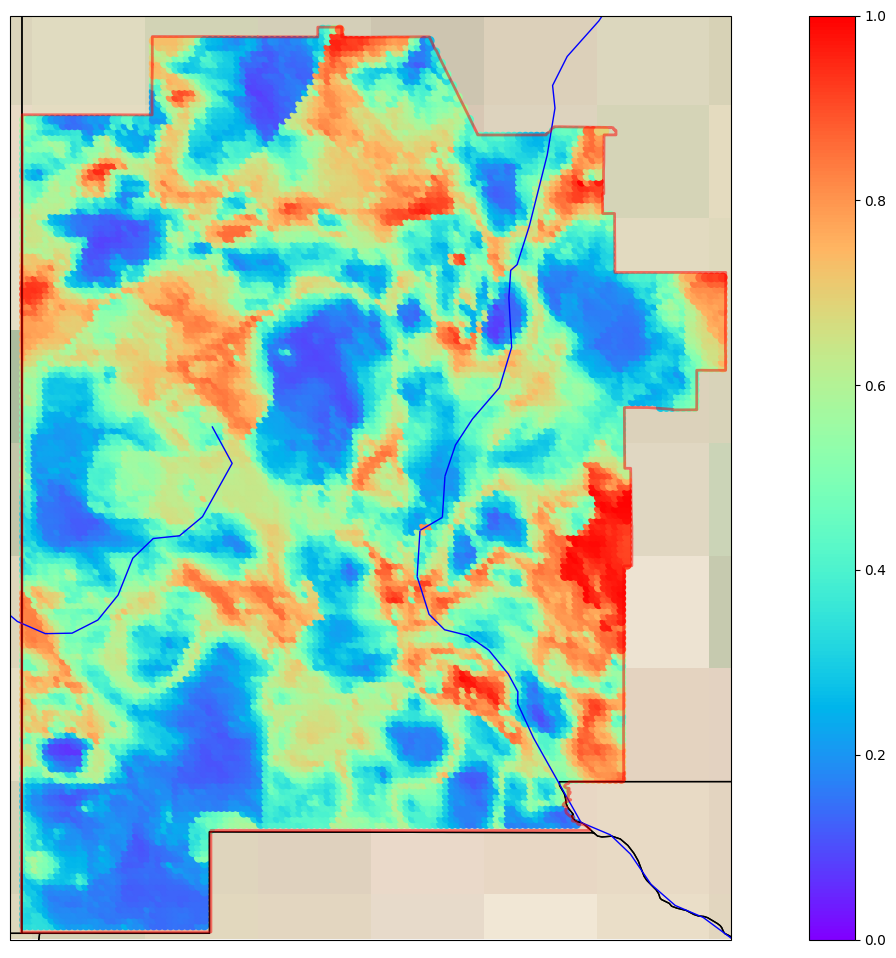
\includegraphics[width=.8\textwidth]{templates/images/Figure-MU_Entropy_Map.png}
\caption[SiGT measurement uncertainty map]
{SiGT measurement uncertainty based on normalized Shannon entropy. Calculations were made on class probability averages after modeling 100 randomly-perturbed realizations with the WDS4 XGB classifier. Values range from 0 for low entropy, low uncertainty (blue) to 1 for high entropy, high uncertainty (red).}
\label{fig:mu_entropy_map}
\end{figure}

XGBoost models, parameterized as described for WDS4 in Table \ref{tab:xgb_tuning}, were trained on the perturbed data sets and used to predict geothermal classifications for the FDS covering the full AOI. After ensemble-averaging the class probabilities at each point, the maximum probability class was selected as the class assignment for the average geothermal gradient classification map. Shannon entropy values calculated from the average class probabilities are shown in Figure \ref{fig:mu_entropy_map}. Figure \ref{fig:mu_masked_pred_map} combines both maps using entropy values >0.7 as a layer mask and assigning increasing transparency with greater entropy for the remaining points.

Interestingly, variations in SiGT values result in high classification uncertainty in many locations across the AOI (Figure \ref{fig:mu_masked_pred_map}). Concentrated areas of uncertainty are observed in the southwest -- an area where silica samples were collected but not many WDS4 well observations are located (Figure \ref{fig:mu_stderr_entropy}). Similarly, large patches of higher entropy appear in the north and just west of the AOI center. Once again, these are under-sampled regions in WDS4 (Figure \ref{fig:mu_stderr_entropy}). It appears that as training data values for SiGT change due to perturbations, thresholds for XGBoost decision trees shift enough to significantly impact the stability of model predictions away from wells. SiGT-related splits will appear near the root node of decision trees based on its dominance over other features for classification importance. Changes to the decision thresholds will thus have a strong cascading effect on the final classification choices for XGBoost models. The problem lies in both the magnitude of SiGT standard errors as well as the sparse sampling of the study area by WDS4 well locations. The degree of uncertainty seen here would likely be reduced if WDS4 included more comprehensive coverage of the study area.

\begin{figure}[!htp]
\centering
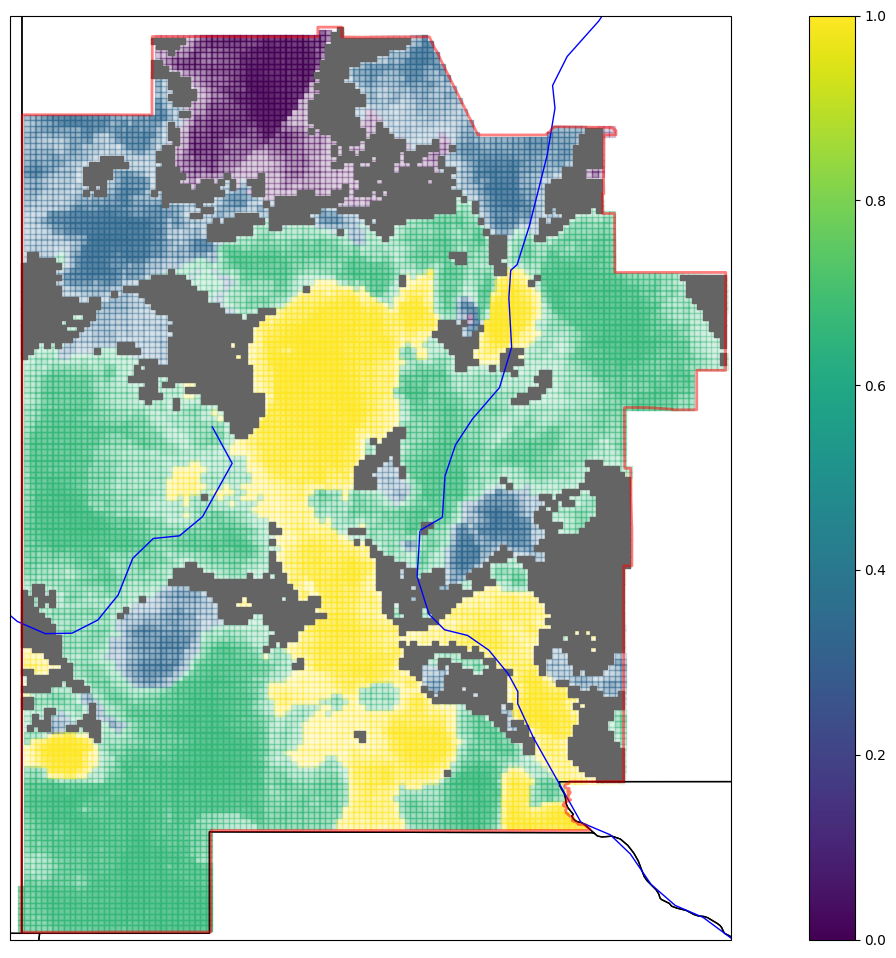
\includegraphics[width=.8\textwidth]{templates/images/Figure-MU_Masked_Average_Gradient_Map.png}
\caption[SiGT measurement uncertainty mask on prediction map]
{Probability-averaged WDS4 XGB prediction map with SiGT measurement uncertainty masking. Normalized entropy values (>0.7) are grayed out, all others determine transparency of the colored scatter plot. Transparency increases from none at entropy values close to 0, to full for entropy values close to 1. The background topographic raster has been removed to better visualize the transparency effect.}
\label{fig:mu_masked_pred_map}
\end{figure}

\begin{figure}[!htp]
\centering
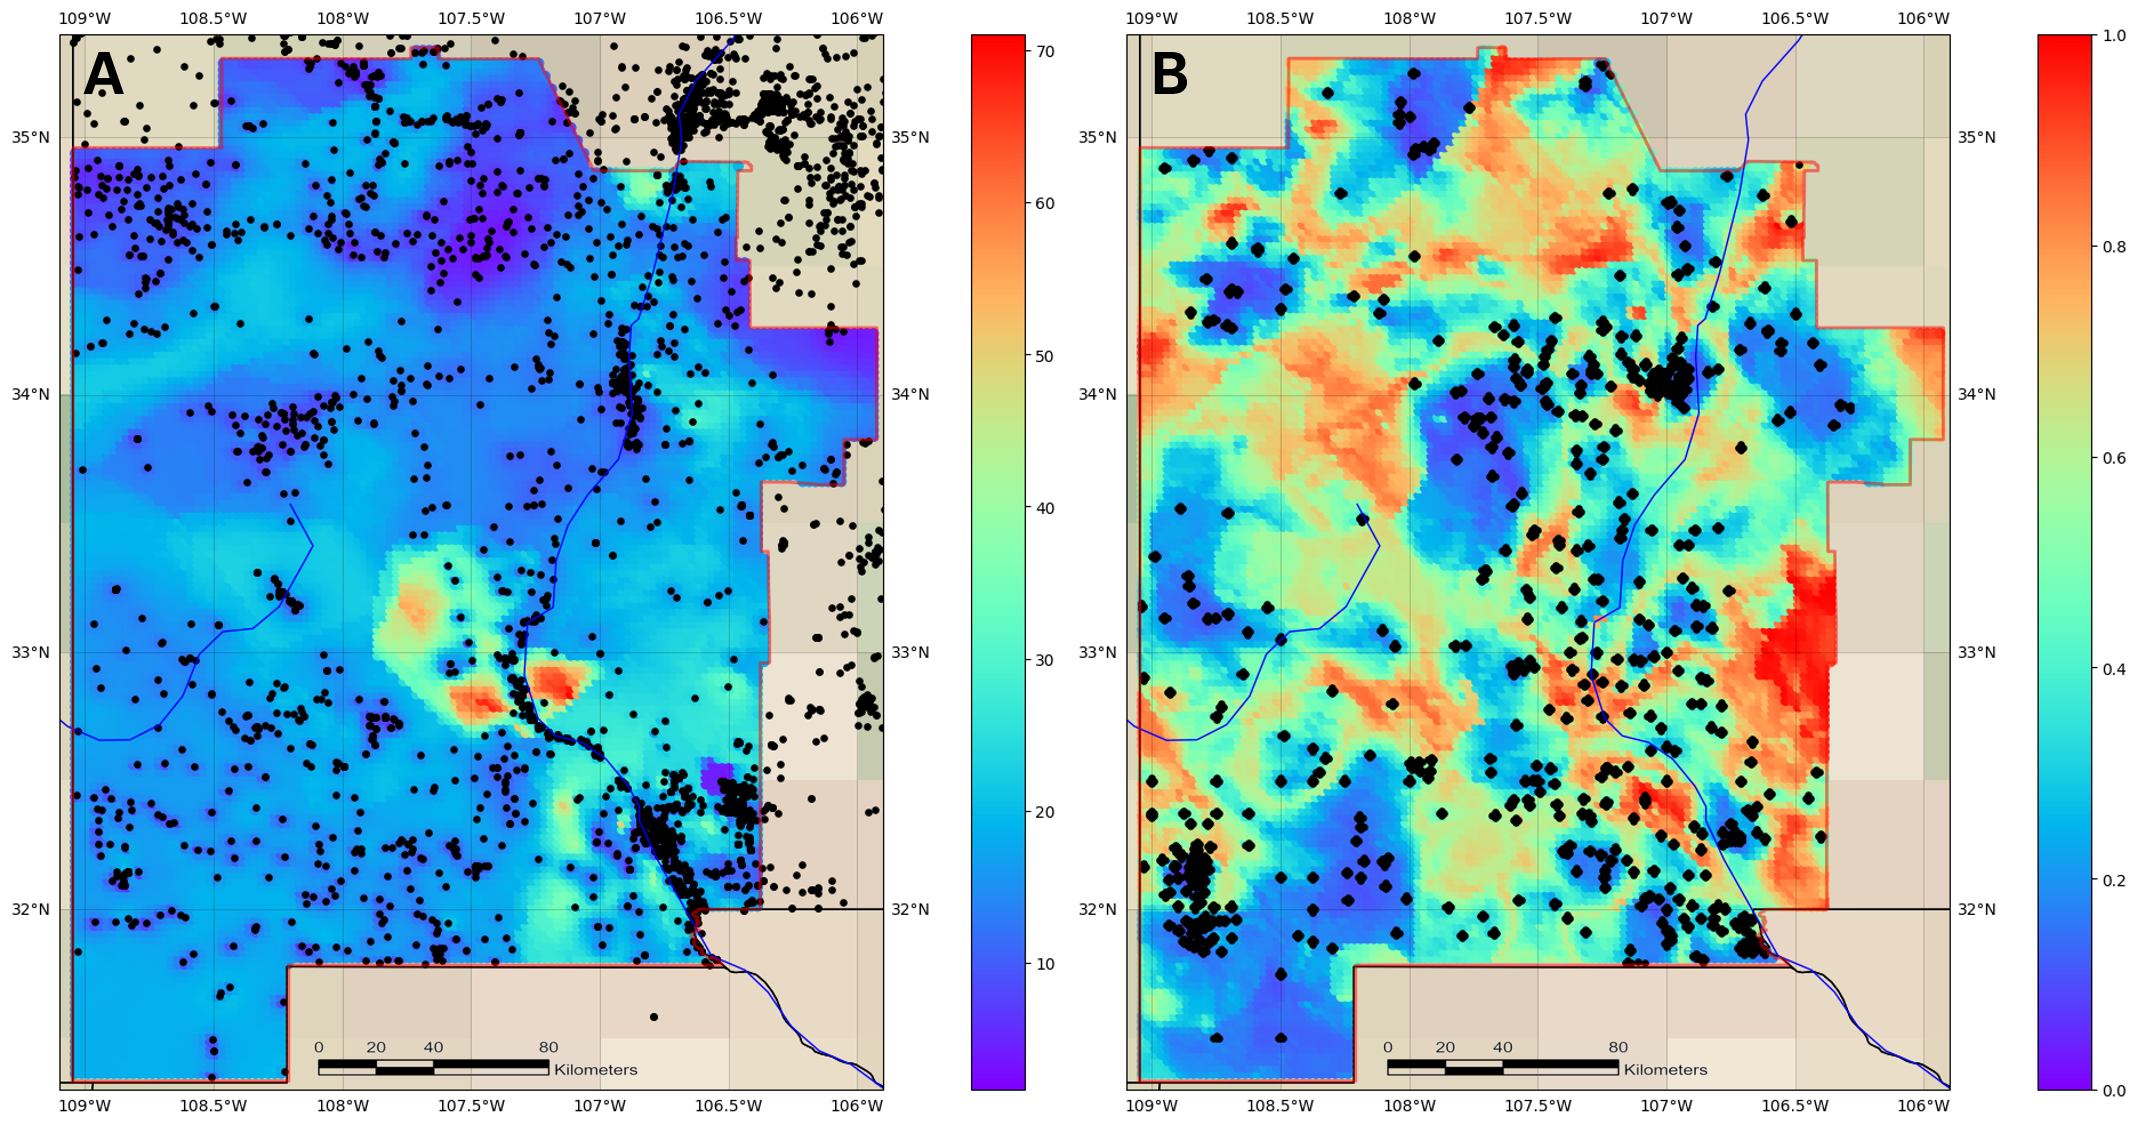
\includegraphics[width=\textwidth]{templates/images/Figure-MU_StdErr_vs_Uncert.png}
\caption[SiGT standard error and model entropy]
{A. SiGT standard error map derived from kriging operation in ArcGIS. Block dots show the locations of silica concentration samples that are the feature source data. B. WGS4 XGB measurement uncertainty entropy map. Black circles indicate well locations in WDS4 used for training the final XGB classifier. }
\label{fig:mu_stderr_entropy}
\end{figure}

\section{Recap}\label{ch5:recap}
\textbf{TO BE COMPLETED}